\documentclass[12pt]{article}

\title{Fires Far Away: A Solitaire Journey}
\author{John Conway}

%PACKAGES
\usepackage[utf8]{inputenc}    
\usepackage[T1]{fontenc}
\usepackage[table]{xcolor}
\usepackage{ebgaramond}
\usepackage[left=0.75in, right=0.75in, top=0.75in, bottom=0.5in]{geometry}    
\usepackage{tcolorbox}    
\usepackage{sectsty}
\usepackage{tikz}    
\usepackage{graphicx}
\usepackage{framed}
\usepackage{multicol}
\usepackage{pdfpages}
\usepackage{titlesec}
\usepackage{lipsum}
\usepackage{tocloft}
\usepackage{pbox}
\usepackage{array}
\usepackage{tabularx}
\usepackage{eso-pic,graphicx}
\usepackage[hidelinks]{hyperref}

%SETTINGS
\setlength{\columnsep}{2em}
\hypersetup{hidelinks}

%COMMANDS
\newcommand{\refto}[1]{\hyperlink{#1}{\textbf{#1}}}
\newcommand{\makeref}[1]{\hypertarget{#1}{\textbf{#1}}}
\newcommand{\reftoit}[1]{\hyperlink{#1}{\emph{#1}}}
\newcommand{\makerefit}[1]{\hypertarget{#1}{\emph{#1}}}
\newcommand{\refton}[1]{\hyperlink{#1}{#1}}
\newcommand{\makerefn}[1]{\hypertarget{#1}{#1}}

% LaTeX counter interface for \rownum
% ---
\makeatletter
\@ifundefined{c@rownum}{%
  \let\c@rownum\rownum
}{}
\@ifundefined{therownum}{%
  \def\therownum{\@arabic\rownum}%
}{}
\makeatother

%COLUMNS
\newcolumntype{L}{>{\raggedright\arraybackslash}m{5cm}}
\newcolumntype{C}{>{\centering\arraybackslash}m{5cm}}

%DOCUMENT
\begin{document}
\newpage 
\thispagestyle{empty}
\pagenumbering{gobble}
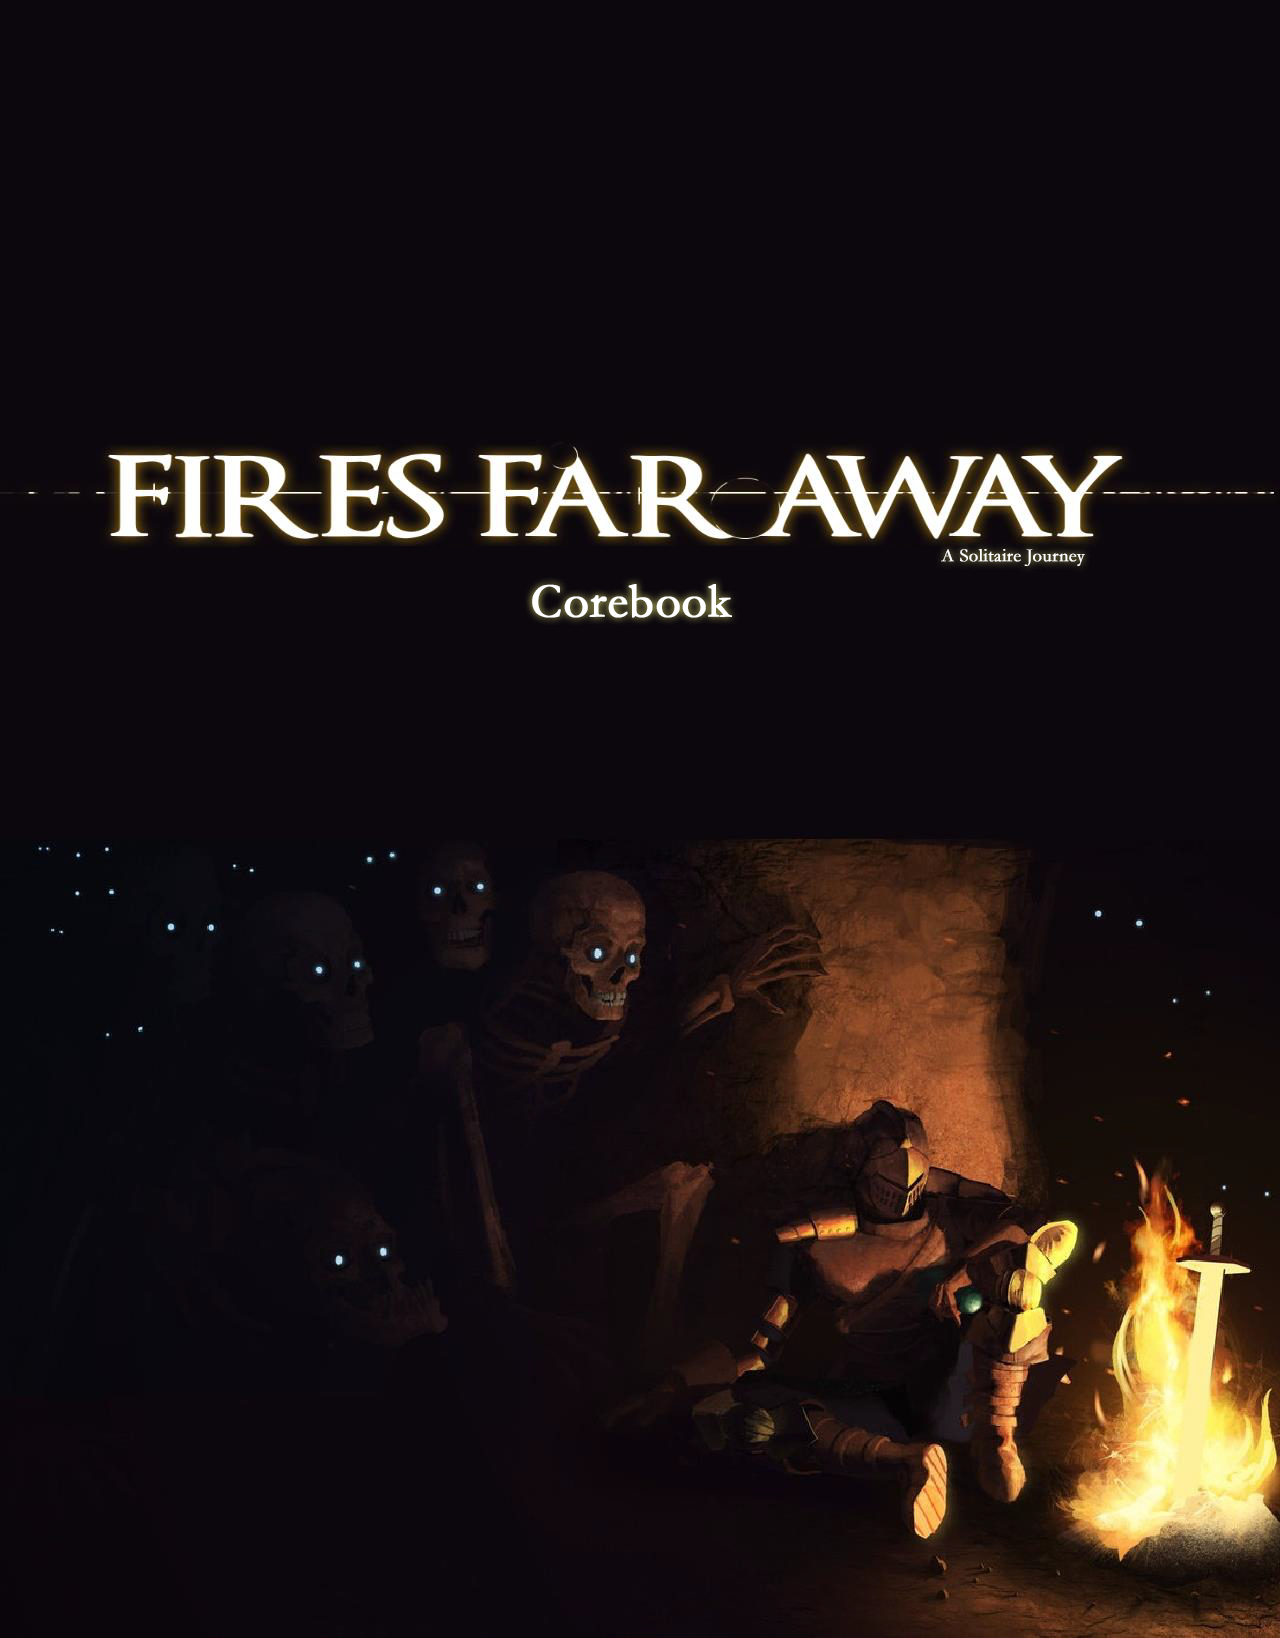
\includepdf{misc/cover.pdf}

\newpage

\AddToShipoutPictureBG{
\includegraphics[width=\paperwidth,height=\paperheight]{misc/background.pdf}}
\begin{multicols*}{2}
\setlength\parindent{0pt}
\pagenumbering{arabic}
\setcounter{page}{1}

\phantomsection
\addcontentsline{toc}{section}{Introduction}
\section*{Introduction}
\emph{Fires Far Away: A Solitaire Journey} is a single-player conversion of the original Fires Far Away: a pen \& paper homebrew developed by an anonymous poster(s?) on the 4chan /tg/ board. As of the Spring of 2021, the original rulebooks are still available at \url{https://1d4chan.org/wiki/Fires_Far_Away}.

\section*{Themes}
\subsection*{Scarce Vistas}
The player is not inundated with illustrations, explanations, or exposition. An imagination will have to paint in the whites left reserved by the scenario.

\subsection*{Stern Diktats}
The game is designed to be stern, but not cruel. The goal is to challenge the player’s mind and rattle their playstyle, not crush their character in a random or merciless fashion.

\subsection*{Rigid Chances}
Like the original homebrew, \emph{Fires Far Away: A Solitaire Journey} eschews dice rolls as a resolution mechanic whenever possible. A small amount of randomness is present, but the game favors flat success conditions. The outcome of the character’s actions is not dependent on rolling well, but rather playing well to the rolls.

\subsection*{Vorpal Encounters}
No scenario should contain any throwaway encounters or “trash mobs”. Each encounter should be a puzzle in and of itself, pitting the character against a mortal and uniquely challenging threat.

\subsection*{Beggared Allowances}
All mechanics are based around low arithmetic, making them easily tracked via tokens, coins, pencil marks, beads, or even fingers. No need for an abacus or similar such apparatus.

\subsection*{Beleaguered Narratives}
The player is not expected to surmount every obstacle or defeat every enemy; they aren’t even expected to survive every battle. A scenario is a story as much as it is a challenge, and every well-told tale traverses both valleys and summits.

\subsection*{Convoluted Timelines}
Unique to \emph{Fires Far Away: A Solitaire Journey}, the player is not likely to experience a scenario in any canonical order. The furtive element of randomness rears its head here; each scenario is broken into chapters that are played in order of draw.

\subsection*{Unreliable Recollections}
As the player makes their way through a scenario, they will occasionally be asked to take notes on their actions’ outcomes. These notes are referenced later in play, even if that means being referenced earlier in the scenario’s timeline. The same holds true for the character’s equipment and advancements, which have a habit of flaunting the laws of time and space. Memories in this game are somewhat unreliable, so players should try not to grow too attached to them.

\vfill

\section*{Legal}
Fires Far Away was not released under any license or copyright. \emph{Fires Far Away: A Solitaire Journey} is released under the CC BY-NC-SA 3.0 US license. In other words, this is an “open source” item. Additions and modifications are welcome as long as they’re non-commercial.

\section*{Credits}
Version: 0.99\\
\textbf{Original Homebrew:} Unknown\\
\textbf{Cover Art:} sstarkm\\
\textbf{Solitaire Conversion:} John Conway\\
\emph{And special thanks to our playtesters!}

\newpage

\renewcommand*\contentsname{Table of Contents}
\tableofcontents
\subsubsection*{And Attached Sheets...}
\vfill

\pagebreak

\section{Game Structure}
\emph{Fires Far Away: A Solitaire Journey} is played in three phases: \textbf{character creation}, \textbf{scenario resolution}, and the scenario’s \textbf{\emph{prestige}}.
\subsection{Character Creation}
This phase is unique to each scenario or campaign. The scenario book will lead the player through the process of creating a character, including their starting statistics, equipment, and other pertinent details. This might be done through selecting a background, answering questions, rolling dice, overt point buys, or any number of creative methods.
\begin{tcolorbox}
\textbf{Note:} The scenario may alter some statistics, or add new ones. A thoughtful scenario will provide the player with a customized character sheet on which to record these new details.
\end{tcolorbox}

\subsection{Scenario Resolution}
Each scenario is split into several chapters, and each chapter functions as a self-contained adventure which both influences—and is influenced by—the events in its sister stories.

\subsubsection*{Scenario Setup and Resolution}
Complete the following steps:
\begin{enumerate}
\item Refer to the scenario book for a list of chapters, and any special setup instructions
\item Write each chapter’s number or symbol on the face of a separate index card
\item Gather these cards into a deck, and shuffle them face-down
\item One by one, draw each card from this chapter deck and resolve the written chapter
\item After each chapter is resolved, discard its card and draw the next one
\item When the entire chapter deck is exhausted, continue onto the scenario’s \emph{prestige}
\end{enumerate}

\subsubsection*{What Carries from Chapter to Chapter?}
As a general rule, everything is retained unless the scenario specifies otherwise. This includes equipment, character advancements, and any permanent notes from previous chapters.\\
Some equipment and items are \reftoit{Ephemeral}, and are erased after the chapter in which they are found. The player should never erase anything else from their character sheet or stash, even if it seems asinine that they would still be available. The character’s memory of the scenario’s events is hazy at best; some logical inconsistencies are to be expected.

\subsection{The \emph{Prestige}}
In the climax of each scenario, the fruits of the character’s toils are finally revealed. The knotted timeline is unraveled, answering some questions and perhaps presenting more. The logical inconsistencies of the scenario’s telling become clearer in hindsight, and the player is asked to forgive their character’s mind for its follies and fabrications.\\
The scenario’s \emph{prestige} may or may not contain additional encounters or CYOA segments.

\subsubsection*{Campaign Play}
Some scenarios are merely links in the chain of a greater campaign, and their \emph{prestige} is used to sand out the rough edges of the matryoshka in preparation for the next layer. Unlike chapters, the player is expected to play a campaign’s scenarios in sequential order. Unless instructed otherwise, the player should assume that all their equipment and advancements will be retained upon progressing to another scenario in the same campaign.\\
Scenarios that are not part of a campaign are meant to be one-shots, and are not balanced for playing with the veteran of a separate adventure. 

\vfill
\pagebreak

\subsection{Required Materials}
In order to facilitate smooth gameplay, it is recommended for the player to have at a minimum:
\begin{itemize}
\item Both this corebook and a scenario book (digital copies are perfectly fine)
\item A pencil
\item A large eraser (for big mistakes)
\item 8 six-sided dice
\item A fresh pack of index cards or scratch paper
\item A bowl of coins, beads, or other small and discrete tokens
\item Printed copies of the character, status, and record sheets (and optionally the encounter quick reference sheet)
\item 3 double-sided copies of the Hexagon-Tiled Map
\item A card table or other mid-sized playing surface
\end{itemize}
What materials the player lacks can be substituted with a pencil—or a good memory, but preferably the pencil.

\subsubsection*{The Character and Status Sheets}
The character sheet is for tracking the crunchy aspects of the character, such as their statistics and equipment. It is mostly written in pencil.\\
The status sheet is used for the more dynamic and token-heavy mechanics such as the \refto{HP} slots, \refto{FP} pool, and \reftoit{sinks}.

\subsubsection*{Dice}
The player will need a large number of six-sided dice due to the game’s \reftoit{stamina pool} system. Depending on the character’s \refto{END} stat, they may need to keep six or more dice reserved for \refto{SP} dice. In addition, they will need two more dice for rolling on the encounter table(s).\\
If the player does not have access to this many dice, they can compensate with tokens. Cut some index cards into tokens with the number range one through six written on them, and use them to track dice scores.

\subsubsection*{The Hexagon-Tiled Map}
While it may be tempting to forgo printing physical copies of the map, it is vital for playing the game’s encounters. It’s recommended to print the map double-sided (and draw lightly) to save paper. Having some method of representing entities on the map is also necessary; the width of each hex is just enough for an American quarter-dollar or 25mm base miniature.

\subsubsection*{Index Cards}
Index cards are a versatile tool. They’re normally used for chapter cards, enemy sheets, and \reftoit{Shield Up!} tokens. But they can also be cut up to make condition tokens, or representations for entities on the Hexagon-Tiled Map.

\subsubsection*{The Record Sheet}
Occasionally, the player will be asked to take notes. They will also need to keep track of their known attunements and stash contents. This information would best be written on the record sheet, but a notepad or piece of scratch paper will also suffice.

\subsubsection*{\emph{Shield Up!} Tokens}
The player will need at least one token for simulating when an entity has their shield raised. This token needs to be large, because it will be holding damage tokens that would otherwise be assigned to the shielded entity. An index card with \reftoit{Shield Up!} written on it, along with the shield’s stats, will suffice.

\subsubsection*{Tokens}
Tokens are primarily used for keeping track of the game’s counters such as \refto{FP}; charges for items and flasks; and damage.\\
Damage tokens are assigned to \refto{HP} slots, left unassigned on entity sheets, or deposited in \reftoit{sinks}; and this all happens frequently. Tokens will likely be the limiting reagent of the game, so the more of them the player can scrounge up the better. Coinage is very useful for tokens, since it presents an immediately familiar point worth (1 nickel = 5 pennies, for example) and cuts down on the total number of tokens in play.\\
As a last resort, the player can draw symbols or mark tallies in lieu of using tokens.
\end{multicols*}

\pagebreak

\begin{center}
\makebox[\linewidth]{
        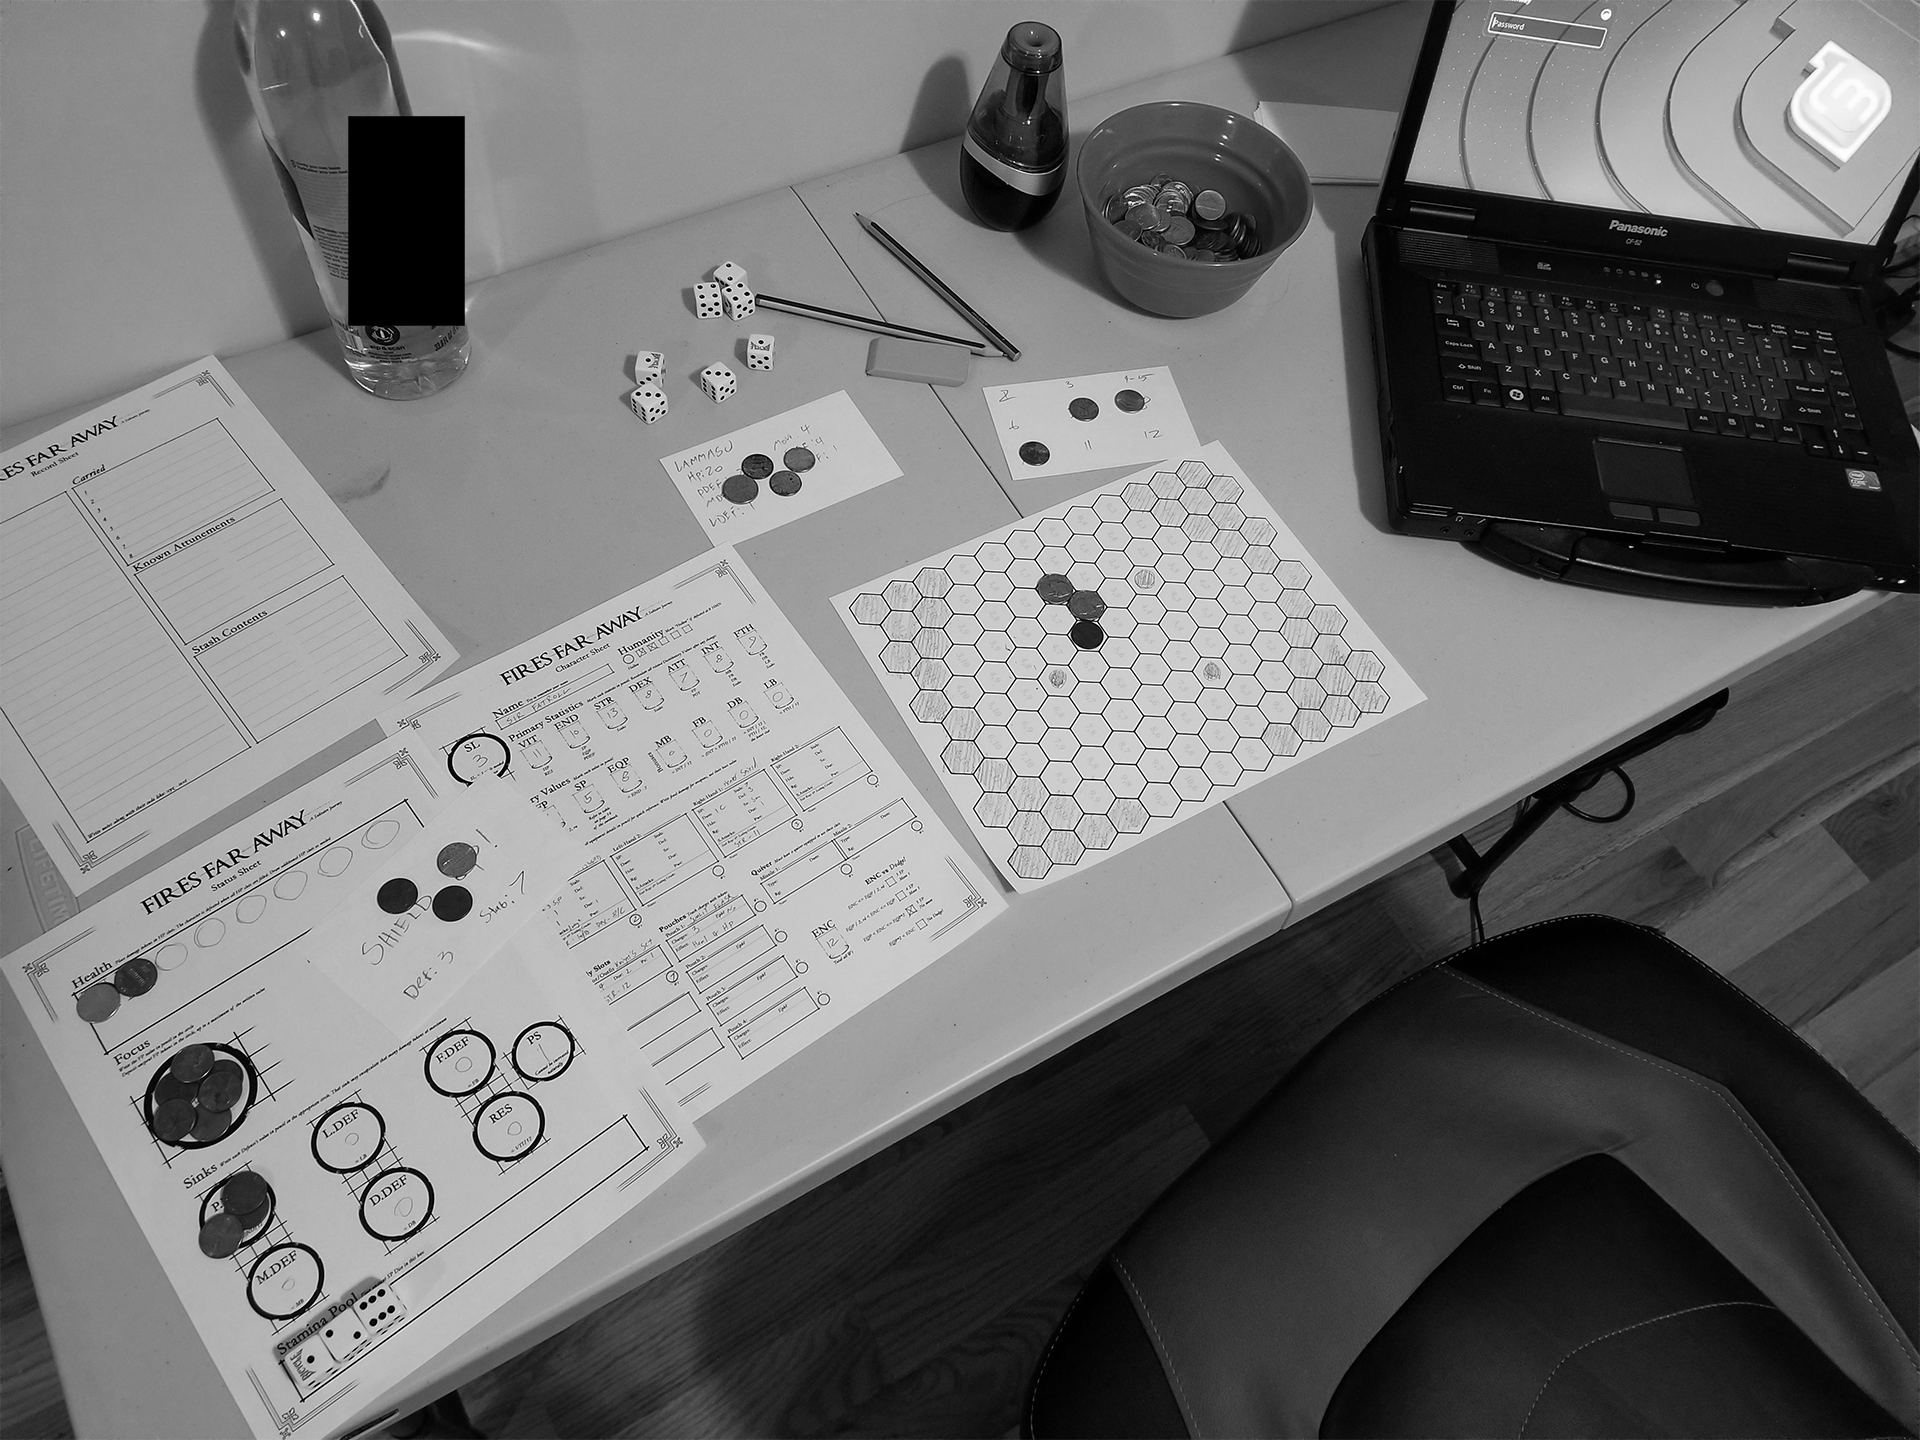
\includegraphics[width=0.8\linewidth]{misc/setup_greyscale.png}
    }
\emph{An example setup using a foldable card table.}

\ \\ \ \\

\makebox[\linewidth]{
        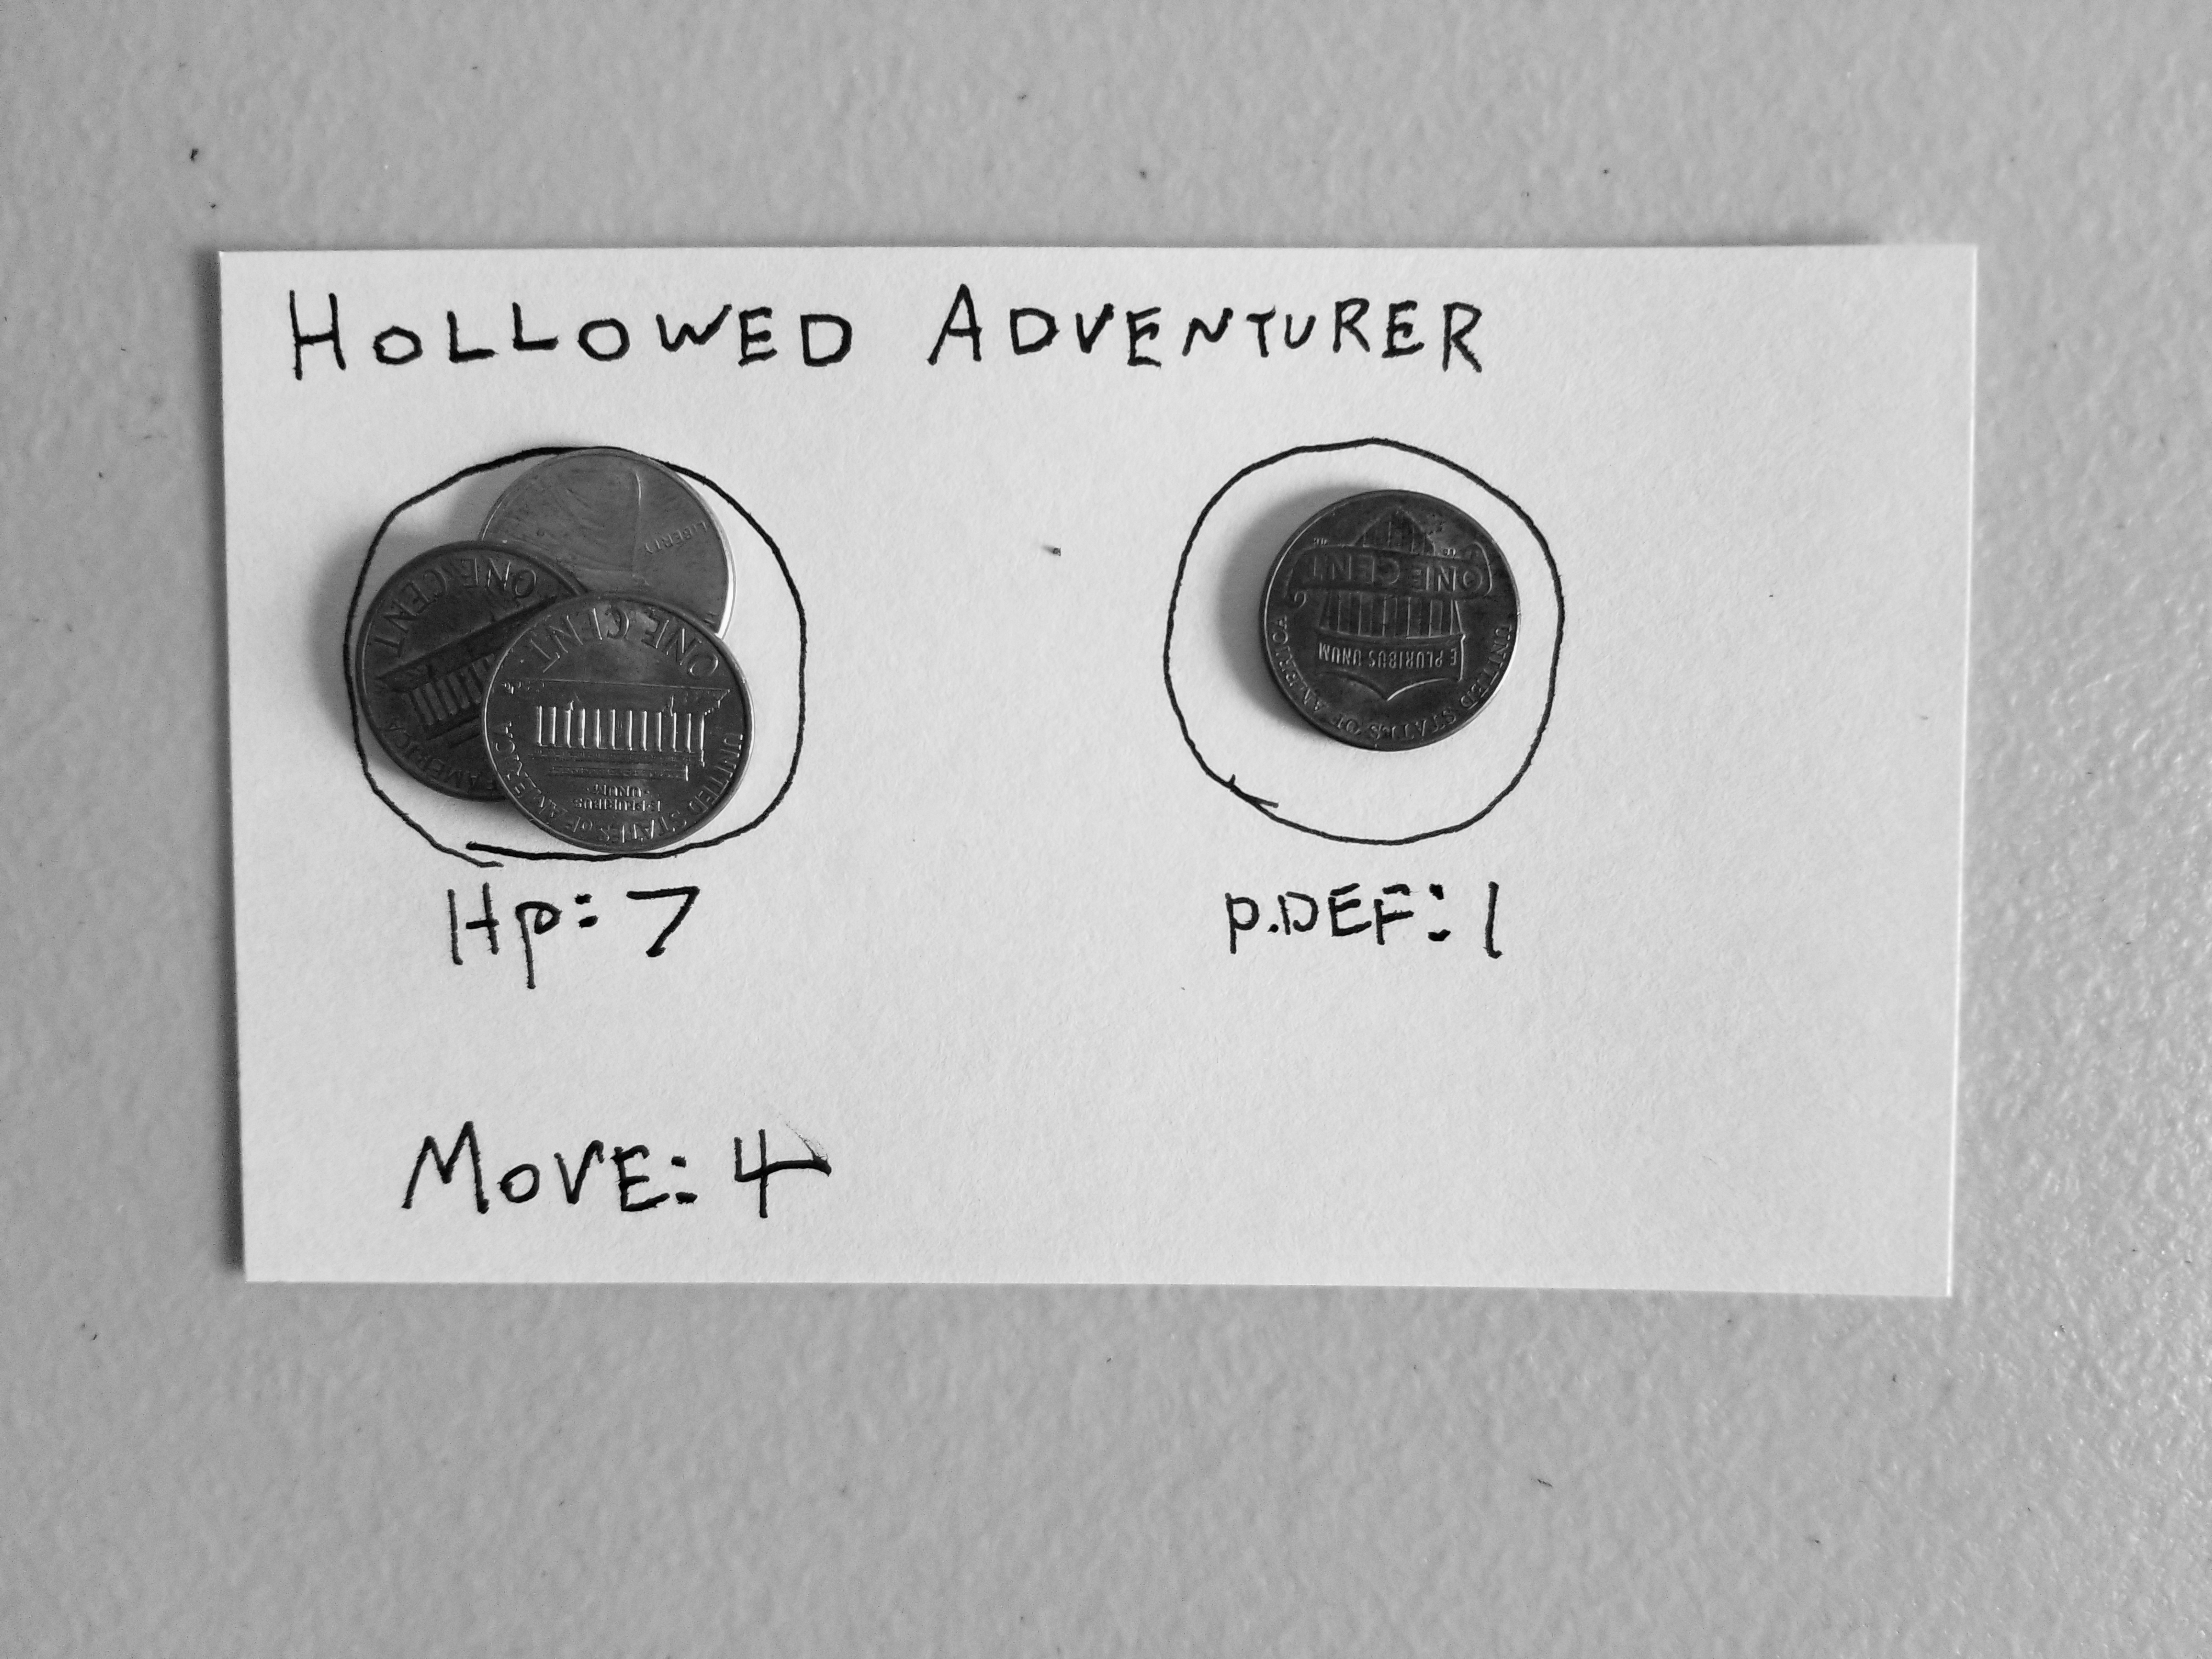
\includegraphics[width=0.8\linewidth]{misc/setup_enemy.jpg}
    }
\emph{An example enemy sheet written on a plain index card.\\
The enemy has taken 4 damage: 3 to its \refto{HP}, and 1 \reftoit{sunk} in \refto{P.DEF}}
\end{center}
\begin{multicols*}{2}

\setlength{\parindent}{0pt}
\section{Rules \& Terminology}
\subsection{General Concepts}
\subsubsection*{Dice Rolls}
All rolls are made using six-sided dice. Since this game only uses one type of die, it is abbreviated as “D”. If a dice roll or dice requirement is prefixed by a number, use that many six-sided dice, i.e: 2D calls for two dice.\\
Do not use a twelve-sided die instead of two six-sided dice; the probabilities would be different.\\
Sometimes the game calls for dice to be re-rolled; this is once per die and the second result is always final.

\subsubsection*{Dice Scores}
The number rolled on a \refto{SP} die is its score. A die cannot have its score split in any way, and its score can only be committed to a single action.\\
The requirements for in-game actions may be written either in number of dice or as a flat score. If an action calls for 1D, it means one \refto{SP} die with any score. So 2D of course calls for two dice of any scores to be spent.\\
A flat number requirement, such as a 6, calls for a minimum of that total score to be spent. This can be achieved by committing either a single die that scored a 6, or by combining any number of \refto{SP} dice whose total is at least 6.\\
A plus sign designates an action that can be overspent for bonus results, i.e: a 5+ means the minimum required score is 5, but that the action provides some sort of extra effect for every score spent over 5. This is typically limited to double the original cost.

\begin{tcolorbox}
\textbf{Note:} If an action calls for a score of 7 or more, it will require at least two \refto{SP} dice to achieve. The difference between the game calling for 2D vs a flat 7 is:\\
1. The 2D can use any two dice regardless of their combined score.\\
2. A 2D action is a Double action. Refer to the Actions \& Reactions section for details
\end{tcolorbox}

\subsubsection*{Learning to Play}
Because \emph{Fires Far Away: A Solitaire Journey} does not have a human gamemaster orchestrating it, the system’s mechanics must act as a substitute. Opponents cannot surprise or challenge a player if that player controls their every move. For this reason, the encounter system is complex--and may be somewhat difficult to learn. In addition to the explanations and gameplay example included in this corebook, the companion scenario--\emph{Everloyal}--contains a tutorial chapter that introduces players to the encounter system via a dripfeed of its mechanics. This companion scenario should be available wherever this corebook was found.

\subsubsection*{Rounding}
In order to minimize crunch, mechanics that involve division have their solutions rounded. The abbreviation \emph{rd} is a reminder that the score must be rounded to the nearest whole number.

\subsubsection*{Recordkeeping}
The player is asked to keep track of a large amount of information throughout a scenario. Dynamic counters such as damage and \refto{FP} are tracked via physical tokens because they are added and removed often, and constantly writing and erasing pencil marks would create an indecipherable mess. Notes and equipment, or less dynamic counters such as \refto{HMN}, are tracked via the pencil.\\
When taking a break from the game, the number and locations of tokens should be written down rather than left to the whims of pets, parents, and gusts of wind.

\subsubsection*{Scenarios and this Corebook}
This corebook should be considered a base set of rules, which are then modified by the scenario-specific ruleset. Just because an item or concept appears in this corebook does not mean it is available in every scenario. When the mechanics of the scenario and corebook differ from each other, always defer to the scenario.

\subsubsection*{Uncertain Mechanics}
If the player is ever uncertain about the specifics of a mechanic, or is flummoxed by a bizarre situation in which two mechanics disagree, they are welcome to \emph{Make Something Up}. It would be preferable if the solution wasn’t chosen by virtue of being the most beneficial to the player.

\vfill
\pagebreak

\subsection{Chapter Concepts}
\subsubsection{Chapter Exploration}
Chapters are often (but not always!) relegated to distinct geographic locations. Some chapters might proceed in a linear fashion, while others may have multiple routes or allow for freeform exploration. It’s also possible for chapters to retain special rules, such as a ticking timer or pursuant enemies. \\
What all chapters share is their CYOA format, with resolutions written on separate pages in non-sequitur order. When progressing through a chapter, the player must remember that their exploration options are limited to only what is listed on the current page.

\begin{tcolorbox}
\textbf{Example:} If the player drops down a cliffside and turns to a page where no option is given to climb back up, then the player cannot turn back to that previous page at the clifftop. Likewise, the character can only take a \reftoit{short reprieve} or access their stash where the chapter specifically allows for that action.
\end{tcolorbox}

When instructing the player on which page to turn to, the scenario will use the format \emph{xx:yz}, where \emph{xx} is the page number, and \emph{yz} are the section and reading.

\subsubsection{Chapter Actions}
When reading through a chapter, a chevron (>) designates a chapter action. Chapter actions are events such as: moving to other locations, marking notes, gaining equipment, or making other decisions--all of which have some in-game effect. Chapter actions are normally optional, but chapter actions marked with double chevrons (>>) are required and \emph{must} be taken.

\subsubsection{Checks}
Occasionally, the chapter may restrict progress or grant the player extra progression options based on a check. This most often comes in the form of gates, where some physical portal is locked until the character acquires its key. Other times this might be a strict stat check, like only allowing a character with 12+ \refto{INT} to make sense of a magical tome. A check may also reference the character’s past actions via their notes.\\

\textbf{Checks Roster:}\\
An option prefaced by \emph{italicized text} designates a check; this is a requirement that must be fulfilled to take its subsequent chapter action. For example, \emph{8+ INT} designates a chapter action that can only be taken by characters with an \textbf{INT} score of 8 or higher. A check might also ask for a note via its code, such as \emph{Note 123a}, or refer to a certain item the character must possess.\\

\emph{AND/OR} can be used to require multiple checks for a chapter action, or at least one of them.\\

A \emph{NOT} means that the player mustn’t meet the check in order to take the subsequent chapter action--it is normally used to prevent the player from redundantly returning to previously encountered readings.\\

The above concepts are formally known as Boolean logic, and all Boolean concepts apply to them. Further information on Boolean logic can be gleaned from an internet search.

\begin{tcolorbox}
\textbf{Example:}\\
>> A required action \\
> An optional action \\
> \emph{XXX:} An optional action that requires \emph{XXX}\\
>> \emph{XXX AND YYY:} An action that \emph{must} be taken if both \emph{XXX} and \emph{YYY} are fulfilled
\end{tcolorbox}

\subsubsection{Finding Equipment}
Throughout a chapter’s CYOA gameplay, the character may be presented with equipment and items. This gear can only be gathered once, even if the character makes repeated trips to the section in which they are available. 

\subsubsection{Notes and Permanent Notes}
The player is frequently asked to takes notes in service of the scenario’s CYOA gameplay. Notes are written along with a code (like \emph{Note 123a - Got key}) and are referenced only by this code to avoid spoilers. Most notes are erased at the end of each chapter to prevent the record sheet from becoming cluttered with information that will never be referenced again.\\
However, notes bracketed by exclamation marks (like \emph{!!123b!! - Killed Patches}) are permanent notes, and may be referenced in other chapters. These are written in a separate section of the record sheet to prevent them from getting erased accidentally.

\subsubsection{\emph{Short Reprieves}}
\hypertarget{short reprieve}{}\hypertarget{short reprieves}{}
Occasionally, a chapter will give the player a chance to take a \reftoit{short reprieve}. This action will:
\begin{itemize}
\item Clear all damage tokens from the character’s \refto{HP} slots
\item Restore all of the character’s \refto{FP} tokens
\item Remove all \reftoit{Static} conditions, unless otherwise stated in that condition’s description
\item Refill the charges for all flasks and items that are not \reftoit{Ephemeral}
\item Repair any Broken equipment
\item Lastly, the character can use a \reftoit{short reprieve} to change attunements; upgrade their \refto{SL}; and is generally a good opportunity to take a break from the game.
\end{itemize}

\subsubsection{Souls \& Soul Advancement}
Souls have their values marked in parentheses (the name of a soul is purely for flavor). Whenever the character obtains souls, that value is added to the total on the character sheet. \\
The character’s \refto{SL} may only be upgraded during a \reftoit{short reprieve}, and if the character is not Hollow. Whenever the character upgrades their \refto{SL}, they may increase any Primary Stat by 1 point. Immediately recalculate all Distributory Values after each \refto{SL} upgrade to ensure the full benefit of the increased stat.\\
The cost of upgrading is \emph{\refto{SL} + 1} souls, where \refto{SL} is the current value.

\subsubsection{The Stash}
\emph{Fires Far Away: A Solitaire Journey’s} gameplay does not revolve around vacuuming dungeon floors. Characters should not be lugging around twenty shortswords in the hopes that they might find some pawn shop that’ll take them. However, the game has taken some precautions for to-be-used equipment. Any equipment or items the character finds can be stored in the stash, as long as that gear isn’t \reftoit{Ephemeral}. The character must have access to their stash in order to store or retrieve its contents. The stash can hold any number of items. Note the stash’s contents on the record sheet.\\
The stash has a habit of popping up now and again in odd locations, especially at sites suitable for a \reftoit{short reprieve}. How the stash makes its way from place to place with all the character’s gear is anybody’s guess.

\begin{tcolorbox}
\textbf{Note:} A \reftoit{short reprieve} does not automatically grant the character access to their stash. The scenario must state that the stash is accessible.
\end{tcolorbox}

\vfill
\pagebreak

\subsection{Encounter Concepts}
\subsubsection{Actions \& Reactions}
Up to two actions may be committed during the character’s Turn by spending \refto{SP} dice from the \reftoit{stamina pool}. Actions come in two main types: Simple and Dynamic. In addition, the \refto{SP} cost of an action might define it as a Free or Double action.\\
The character can commit either two Simple actions per Turn, or one Simple and one Dynamic. The character can perform Simple and Dynamic actions in either order.\\
In addition, the character may commit one Free action (an action with no \refto{SP} cost) per Turn. This Free action may not be committed last, and it does not count towards the character’s action minimum or action limit.\\
Actions with an \refto{SP} cost of 2D are Double actions, and count as taking both actions for the Turn. The character may still commit a Free action before a Double, but not afterwards.
\begin{tcolorbox}
\textbf{Example:} A character might perform two Simple actions during their Turn, such as moving and then loading a crossbow.\\
They could also perform a Simple and Dynamic action in either order, such as moving and then attacking (or vice versa).\\
Or, they could perform a Double action like sprinting.\\
For their Free action, the character might switch to an alternative weapon or catalyst, but only once per Turn and not as their final action.
\end{tcolorbox}
Reactions are committed during the \emph{counterbeat} (the enemy Turn)--after an active enemy’s Move (if any), but before their attack. One reaction may be committed before each and every attack, but only takes effect for that specific attack. This is regardless of whether the character is reacting to multiple attacking enemies, or one enemy committing multiple attacks.\\
There is no limit to the number of reactions a character can commit per \emph{counterbeat}, other than the size of their \reftoit{stamina pool} (and only one reaction per attack).\\
The character may not commit a reaction if the active enemy’s Turn is listed as \reftoit{Sudden}.\\

\vspace*{\fill}
\columnbreak

\subsubsection{Area of Effect Attacks}
Some attacks and attunements specify areas of effect rather than targets. Area of effect attacks can always strike concealment or out-of-range tiles, but at least one impact tile must be visible and within range.\\

\textbf{Examples}:
\begin{center}
\framebox{
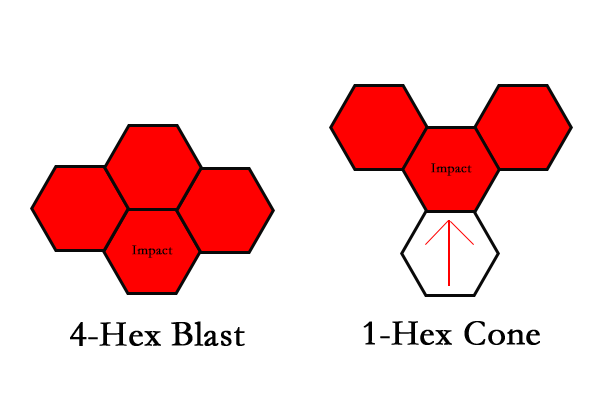
\includegraphics[scale=0.37]{misc/aoes_1.png}}
\framebox{
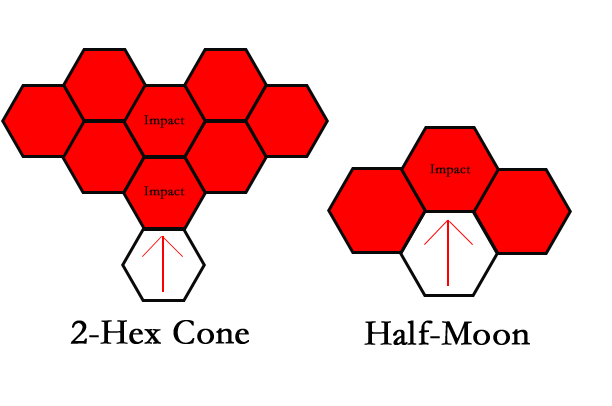
\includegraphics[scale=0.37]{misc/aoes_2.png}}
\framebox{
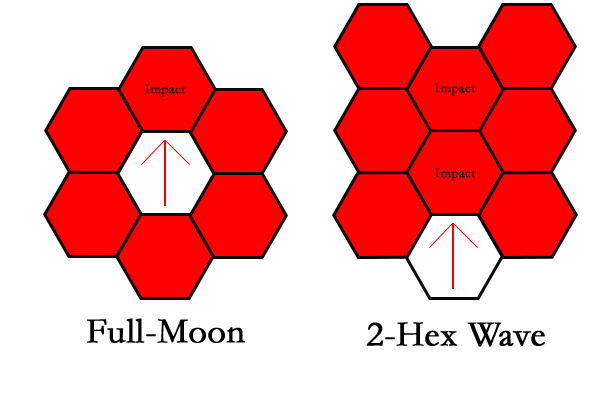
\includegraphics[scale=0.37]{misc/aoes_3.png}}
\end{center}
Expand these examples in a logical fashion for similar patterns such as 3-hex cones or 5-hex waves. Generally, cones expand outward another tile for each addition range while waves always remain three-across.\\
Enemies with complex attack patterns should have visual examples included in their enemy sheet.\\

\pagebreak

Area of effect attacks are blocked by full-cover tiles. When an area of effect attack passes by a full-cover tile, it may not “curve” to reach tiles behind the obstacle.\\
\textbf{Example:}
\begin{center}
\framebox{
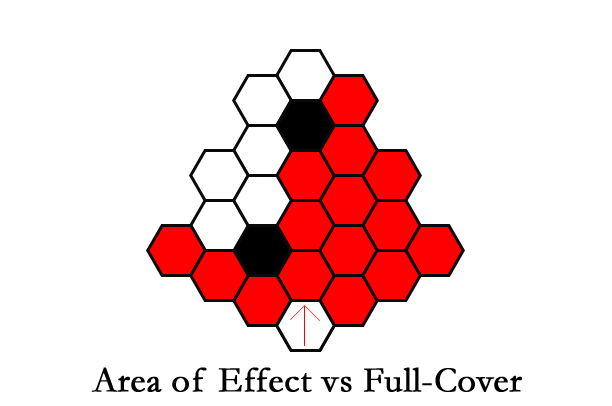
\includegraphics[scale=0.37]{misc/aoe_valid.png}}
\emph{Black tiles are full-cover obstacles. Red tiles are valid targets. White tiles are invalid.}
\end{center}

\subsubsection{Casting Power (PWR)}
\hypertarget{PWR}{}
The \refto{PWR} of an attunement is the combination of the caster’s bonus for that attunement type, and the Power of their catalyst. It alters the effects of an attunement in various ways, such as damage or range.

\subsubsection{Conditions}
All conditions are cumulative unless stated otherwise, meaning an entity can be afflicted with multiple tokens for the same condition. Some conditions may be mitigated via \reftoit{sinks}. Conditions come in three types: \emph{Immediate}, \emph{Time-Limited}, and \emph{Static.}\\

\emph{\textbf{Immediate}} conditions have some instant effect on the afflicted. They do not require a token for recordkeeping, unless they’re being \reftoit{sunk}.\\

\emph{\textbf{Time-Limited}} conditions take effect for as long as at least one token is present on the afflicted’s entity sheet. One \emph{Time-Limited - Turn} token is removed from an entity’s sheet after every Turn. One \emph{Time-Limited - Round} token is removed from all entity sheets at the end of each Round.\\

\emph{\textbf{Static}}\hypertarget{Static}{} conditions take effect for as long as at least one token is present on the afflicted’s entity sheet. These tokens can only be removed by committing certain actions or fulfilling special conditions.

Lastly, some conditions such as Burning and Bleeding produce damage tokens. However, these damage tokens can also be inflicted by attacks that do not inflict their parent condition.
\begin{tcolorbox}
\textbf{Example:} The Bleeding condition produces Bleed damage tokens. The whip weapon also inflicts Bleed damage, but does not inflict the Bleeding condition proper.
\end{tcolorbox}

\subsubsection{Conditions Roster}
\textbf{Blazing:} \emph{Static.} At the beginning of each Turn, the entity receives 1 \reftoit{Unblockable} Burn damage token. Assign this damage as normal (it may be \reftoit{sunk} this Turn).\\
The Blazing token can only be removed via committing the \emph{Roll!} action, or entering certain special tiles.\\
Blazing is a non-cumulative condition; an entity can only be afflicted by 1 Blazing token at a time.\\
Blazing entities do not benefit from concealment, including the effects of darkness.\\

\textbf{Bleeding:} \emph{Static.} At the beginning of the each Turn, before damage is assigned, place 1 Bleed damage token on the entity sheet. Assign this damage as normal (it may be \reftoit{sunk} this Turn).\\
Bleeding is a cumulative condition, but an entity can only be afflicted by 3 Beeding tokens at a time.\\
Bleeding can only be removed via items and some attunements.\\

\textbf{Blinded:} \emph{Time-Limited - Round.} The afflicted entity treats all tiles as if they were concealment. Blinded enemies will not skirt around hazard tiles when moving.\\

\textbf{Broken:} \emph{Static.} Place a Broken token on the afflicted piece of equipment. This equipment provides no effects, and can’t be used. Broken tokens are only removed from equipment during a \reftoit{short reprieve} (or if the equipment regains a Durability \reftoit{sink}). All pieces of equipment including rings and missiles can be broken, but not flasks or miscellaneous items.\\

\textbf{Charmed:} \emph{Time-Limited - Turn.} After the encounter roll, but before the \emph{counterbeat} or any reactions are resolved, the player may make moves and attacks for any Charmed entities. The entity is limited to a Move action and one of its listed attack actions, and it will not obey any encounter roll during a Turn where it is Charmed. Encounter rolls should be made and exhausted regardless.\\

\textbf{\emph{Cursed!:}} \emph{Static.} The character is immediately defeated. The character loses all \refto{HMN}, becomes Hollow, and cannot increase \refto{HMN} or upgrade \refto{SL} while \emph{Cursed!} This condition can only be removed via a secret method.\\

\textbf{Dismounted:} \emph{Static.} A \emph{Mounted} type entity is pulled from their mount. Refer to the entity sheet for details on what this condition entails. This condition is usually permanent.\\

\textbf{Disoriented:} \emph{Instant.} Reduces the character’s \refto{FP} by the specified amount. This condition can be \reftoit{sunk} using \refto{RES} (per Disoriented token, not per \refto{FP} lost).\\

\textbf{Drain:} \emph{Instant.} Drain restores the enemy’s \refto{HP} by the specified amount if its attack assigns any damage tokens to \refto{HP} slots. \\

\textbf{Fear:} \emph{Time-Limited - Turn.} This entity will not move towards the character or attempt attacks with melee weapons. If within 2 tiles of the character at the start of their Turn, an enemy afflicted by Fear will use half their Move value \emph{rd} to move away from the character.\\

\textbf{Flinch:} \emph{Immediate.} The character loses 1 \refto{SP} die with the highest score from their \reftoit{stamina pool}.\\
This condition can be \reftoit{sunk} using \refto{PS}.\\

\textbf{Frozen:} \emph{Static.} The afflicted entity cannot commit to any action except \reftoit{Struggle!} while Frozen, but gains 1 \refto{P.DEF} per Frozen token.\\
Each use of the \reftoit{Struggle!} action removes 1 Frozen token. During a \emph{counterbeat}, any enemy incapable of resolving its encounter roll due to being Frozen will instead perform the \reftoit{Struggle!} action.\\
Frozen entities do not suffer Stun or Flinch from a \reftoit{Guard Break}.\\
Suffering Burn damage will also remove 1 Frozen token per Burn damage.\\

\textbf{Grappled/Eaten:} \emph{Static.} Functions the same as Netted/Webbed, except the character takes routine damage specified by the attack.

\textbf{Hollow:} \emph{Static.} Designates a character that was defeated while having 0 \refto{HMN}. This character cannot upgrade \refto{SL}. This condition is only removed once the character gains \refto{HMN}. In addition, it may affect some chapter options.\\
Gaining \refto{HMN} while Hollow only removes the condition, the character will still be at 0 \refto{HMN} and may hollow again if defeated.\\

\textbf{Knockback:} \emph{Immediate.} The afflicted entity is moved directly backwards from the source of the Knockback by the specified number of hexes.\\
If the afflicted entity is moved onto a hazard tile in this manner, end the Knockback and resolve the effects of the hazard tile.\\
If the Knockback attempts to move the entity into an obstacle or boundary, the entity instead suffers 1 Crush damage per tile moved. If the entity suffers more than 1 Crush damage in this way, then they are also inflicted with Knockdown.\\
This condition can be \reftoit{sunk} using \refto{PS} (at 1 tile per \refto{PS} value).

\begin{tcolorbox}
\textbf{Example:} If an entity suffered Knockback 3 but was already adjacent to an impassable tile, then no damage is inflicted.\\
If the entity suffered Knockback 3, and was moved 2 tiles before striking the impassable tile, then it would suffer 2 Crush damage and Knockdown (it doesn’t matter if the Crush damage was assigned to \refto{HP} slots or not).
\end{tcolorbox}
\textbf{Knockdown:} \emph{Static.} Remove any \reftoit{Shield Up!} token from the afflicted. While knocked down, an entity’s actions are limited to those specifying that they may be committed while knocked down.\\
Any adjacent half-cover obstacles are treated as full-cover while knocked down.\\
During a \emph{counterbeat}, any enemy incapable of resolving its encounter roll due to being knocked down will instead perform the \emph{Get Up!} action.\\
Knocked down entities still occupy their tile(s), but may be crossed over by other entities making a Move action.\\
This condition is non-cumulative, and can be \reftoit{sunk} using \refto{PS}.\\

\pagebreak

\textbf{Maddened:} \emph{Time-Limited - Turn.} A Maddened entity will target the nearest entity during its Turn, friend or foe. If multiple entities are equidistant, the character always takes priority, but otherwise it’s the player’s choice.\\

\textbf{Mute:} \emph{Time-Limited - Round.} A Mute entity cannot use any attunements except for Guts.\\

\textbf{Netted/Webbed}: \emph{Static.} The afflicted entity cannot move as long as one such token is placed on their entity sheet. All other actions cost +1 \refto{SP} per token.\\
Each use of the \reftoit{Struggle!} action removes 1 Netted/Webbed token.\\
During a \emph{counterbeat}, any enemy incapable of resolving its encounter roll due to being Netted/Webbed will instead perform the \reftoit{Struggle!} action.\\

\textbf{Sapped:} \emph{Time-Limited - Round.} The afflicted character rolls 1 less \refto{SP} die per Sapped token on their character sheet.\\

\textbf{Slowed:} \emph{Time-Limited - Round.} All movement taken by this entity has its Move value reduced to Move/2 \emph{rd} to a minimum of 1. This condition is non-cumulative.\\

\textbf{Staggered:} \emph{Time Limited - Turn.} The character can only perform 1 action (Simple or Dynamic) during their \emph{beat} while Staggered.\\
This condition can be \reftoit{sunk} using \refto{RES}.\\

\textbf{Stunned:} \emph{Time-Limited - Turn.} Remove \reftoit{Shield Up!} The afflicted entity may not commit to any actions or reactions while Stunned.\\
A Stunned character with no \refto{SP} dice remaining will still end the Round and re-roll their \reftoit{stamina pool}, and will begin the next Round afflicted by this condition.\\
This condition is non-cumulative.\\

\textbf{Withering:} \emph{Time-Limited - Round.} Withering tokens can use \refto{D.DEF} as a \reftoit{sink}. If the status sheet contains 3 Withering tokens outside of the \refto{D.DEF} \reftoit{sink} at any time, immediately remove all Withering tokens from the status sheet and afflict the character with the \emph{Cursed!} condition.

\subsubsection{Damage}
Most incoming damage tokens are immediately assigned to \refto{HP} slots unless they’re mitigated through \reftoit{Shield Up!}, a \reftoit{sink}, or reactions such as \reftoit{Dodge!} Refer to those mechanic’s sections for details.\\
Some damage types, such as Poison, accumulate on the entity sheet and trickle into \refto{HP} slots each Turn. This often gives the entity the chance to address these tokens before they become wounds, i.e: drinking an antidote to remove unassigned Poison tokens.\\
When all of an entity’s \refto{HP} slots are filled with tokens, it is defeated and removed from the encounter.

\subsubsection{Damage Modifiers Roster}
Incoming damage can be modified to prevent some or all mitigation.\\

\textbf{\emph{High:}} A \makerefit{High} attack cannot hit entities that are knocked down.\\

\textbf{\emph{Inevitable:}} \makerefit{Inevitable} refers to attacks that cannot be mitigated through any means: \reftoit{sinks}, dodging, blocking, or parrying. This damage is assigned directly to \refto{HP} slots.\\

\textbf{\emph{Magical:}} \makerefit{Magical} refers to physical attacks that have been modified with magic. They can only use the \refto{M.DEF} \reftoit{sink}, but can still be placed on \reftoit{Shield Up!} tokens.\\

\textbf{\emph{Unblockable:}} \makerefit{Unblockable} refers to attacks whose damage tokens cannot be placed on a \reftoit{Shield Up!} token. This does not prevent them from being assigned to \reftoit{sinks}.\\

\textbf{\emph{Undodgeable:}} \makerefit{Undodgeable} refers to attacks that cannot be mitigated via the \reftoit{Dodge!} action.\\

\textbf{\emph{Unparryable:}} \makerefit{Unparryable} attacks cannot be parried or riposted, but can still be dodged or placed on a \reftoit{Shield Up!} token. It usually refers to natural attacks, such as bites and claws.\\

\textbf{\emph{Unsinkable:}} \makerefit{Unsinkable} refers to damage tokens that cannot be encapsulated by a \reftoit{sink}. This does not prevent them from being assigned to a \reftoit{Shield Up!} token.

\subsubsection{Damage Types Roster}
\textbf{Acid/Breaking:} For all Acid tokens dealt to the character in a single attack, at least 1 such token must be assigned to an available Durability \reftoit{sink}. The player may assign all Acid tokens to Durability \reftoit{sinks} in this manner. If there are no Durability \reftoit{sinks} available, then at least 1 Acid token must be used to afflict a currently equipped piece of gear with the Broken condition.\\
Acid tokens that are not assigned to Durability \reftoit{sinks}, or do not break equipment, are assigned to \refto{HP} slots as normal. Acid is always \reftoit{Unsinkable} outside of Durability.\\
Breaking damage functions the same as Acid, except it can never be assigned to \refto{HP} slots.\\
For enemies, Acid/Breaking will permanently reduce their \refto{P.DEF}, or their shield’s Durability if the damage is assigned to \reftoit{Shield Up!}\\

\textbf{Bleed:} Bleed damage is always \reftoit{Unblockable}, and can only use \refto{RES} as a \reftoit{sink}.\\
Bleed tokens are never immediately assigned to \refto{HP} slots. While an entity sheet contains unassigned Bleed tokens, assign 2 such Bleed tokens to \refto{HP} slots every Turn.\\
Bleed tokens assigned to \refto{HP} slots are cleared after the end of an encounter.

\begin{tcolorbox}
\textbf{Note:} Use some method to distinguish Bleed tokens, such as a differently colored token or flipping the coin upside down, as a reminder to remove them after the encounter.
\end{tcolorbox}

\textbf{Burn:} Burn damage can only use \refto{F.DEF} as a \reftoit{sink}.\\

\textbf{Dark:} Dark damage can only use \refto{D.DEF} as a \reftoit{sink}.\\

\textbf{Magic:} Magic damage can only use \refto{M.DEF} as a \reftoit{sink}. This includes any Slash, Crush, or Pierce attacks that have been modified to become \reftoit{Magical}.\\

\textbf{Physical}: These three types of damage—Slash, Crush, and Pierce—are all considered Physical damage. Some enemies may have increased defenses against a specific type of Physical damage. A weapon’s damage type(s) determines what sort of attacks can be committed, i.e: a blunt weapon such as a mace cannot use slashing or piercing attacks. All three Physical damage types may use \refto{P.DEF} as a \reftoit{sink}.

\textbf{Poison:} Poison damage can only use \refto{RES} as a \reftoit{sink}. A maximum of 1 Poison token may be assigned to \refto{HP} in a single attack. While an entity sheet contains unassigned Poison tokens, assign 1 such Poison token to an \refto{HP} slot at the beginning of every Turn.\\

\textbf{Smite:} Smite damage can only use \refto{L.DEF} as a \reftoit{sink}.\\

\textbf{Toxic:} Toxic damage can only use \refto{RES} as a \reftoit{sink}. A maximum of 1 Toxic token may be assigned to \refto{HP} in a single attack. While an entity sheet contains unassigned Toxic tokens, assign 2 such Toxin tokens to \refto{HP} slots at the beginning of every Turn.

\subsubsection{Darkness}
In dark encounters, all tiles past range 2 are concealment. With a lit light source, this range is expanded to 5 tiles, but the light-holding entity is not concealed.

\subsubsection{\emph{Guard Break}}
\hypertarget{Guard Break}{}
Shields can block a limited number of damage tokens per Round, determined by the shield’s Stability stat. When a shield blocks an additional token past its Stability, the entity loses \reftoit{Shield Up!} and suffers Stun, Flinch, and 1 Breaking damage on the shield. Any extra damage is assigned as normal. Suffering \reftoit{Guard Break} does not remove any tokens from \reftoit{Shield Up!}

\subsubsection{Light Sources}
Light sources can either come from equipment or attunements. To benefit from an equipped light source, that light source must be currently held and lit.\\
Unequipping a light source during an encounter will douse it (it must be lit again).

\subsubsection{\emph{Lock-On}}
\hypertarget{Lock-On}{}
Attacks with \reftoit{Lock-On} can maneuver towards the target via whatever route they find necessary. \emph{Lock-On} attacks can also target enemies in concealment, and ignore \reftoit{Dodge!}

\subsubsection{Movement}
Movement values are given as a flat number. A movement action may move up to that number of tiles. A hyphenated value such as 1-2 designates some minimum necessary movement for an action.

\subsubsection{Overspent Actions}
When the \refto{SP} cost of an action is denoted with a + sign, it can be overspent up to double the original \refto{SP} cost.

\subsubsection{Ranged Attacks}
Attack ranges are given as flat numbers representing the attack’s maximum distance in tiles. For ranges with hyphenated numbers, such as 2-3, the first number represents the attack’s minimum range.\\
Ranged attacks that are not \reftoit{Lock-On} cannot curve around full-cover obstacles or entities. When plotting the route for a non \reftoit{Lock-On} ranged attack, there must be a direct line of sight from attacker to target regardless of number of tiles travelled.\\
To check difficult calls, simply place a pencil or other straight-edged object from the center of the attacker to the center of the target tile. If the straight-edge does not cross through a tile containing an entity or full-cover, then the attack is valid. The attack is only blocked if it were to pass through two separate edges of the occupied tile; simply skirting an edge will not invalidate the attack.\\
\textbf{Example:}
\begin{center}
\framebox{

\includegraphics[scale=0.3]{misc/ranged_invalid.png}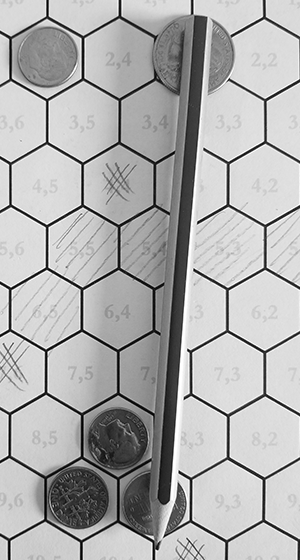
\includegraphics[scale=0.3]{misc/ranged_valid.png}}\ \\
\emph{The tails-up dime (left example) is an invalid target, as the heads-up dime is in the way. The penny (right example) would be a valid target for a ranged attack.}
\end{center}
Ranged attacks without \reftoit{Lock-On} cannot target tiles in or past concealment, but may still strike concealed tiles via any area of effect.\\
Ranged melee refers to melee attacks that occur at range, such as spear thrusts or some large weapons. Although these attacks must obey ranged targeting rules, they are still considered melee and may be parried.

\subsubsection{Rounds \& Turns}
A Round refers to a break in the encounter that occurs when the character re-rolls their \reftoit{stamina pool}. This event is also used for other mechanics, such as \emph{doom events} and some conditions.\\
A Turn refers to a \emph{beat} or \emph{counterbeat}. When this corebook uses Turn in a possessive sense, it is referring to either the character’s \emph{beat} or the enemy’s \emph{counterbeat.} When dealing with Turn-limited trickling damage tokens, such as Bleed or Toxic, they are only assigned on the entity’s Turn.

\subsubsection{\emph{Shield Up!}}
\hypertarget{Shield Up!}{}
Shields are used by committing the \reftoit{Shield Up!} action, which adds a \reftoit{Shield Up!} token to the entity sheet. While \reftoit{Shield Up!} is present, the shielded entity places all incoming damage on this token--up to the shield’s Defense value per attack. The entity may not elect to forgo blocking any attacks in this manner. Damage tokens that are listed as \reftoit{Unblockable} or \reftoit{Inevitable} cannot be placed on the \reftoit{Shield Up!} token.\\
If the number of damage tokens on a \reftoit{Shield Up!} token ever exceeds the shield’s Stability, that entity will suffer an immediate \reftoit{Guard Break.}\\
If knocked down, the entity can still add a \reftoit{Shield Up!} token to their entity sheet, and it will not be removed by performing the \emph{Get Up!} action.\\
If the entity commits any action, remove the \reftoit{Shield Up!} token unless instructed otherwise.\\
Remove all damage tokens from \reftoit{Shield Up!} at the end of every Round.\\
Unequipping a shield or committing Lower Shield will not clear it of damage tokens.

\begin{tcolorbox}
\textbf{Note:} Remember that the \reftoit{Shield Up!} token is not a \reftoit{sink}.
\end{tcolorbox}

\subsubsection{\emph{Sinks}}
\hypertarget{sink}{}\hypertarget{sunk}{}\hypertarget{sinks}{}\hypertarget{Sinks}{}
\reftoit{Sinks} refers to the mechanic by which entities can avoid assigning damage to \refto{HP} slots or suffering certain conditions. \reftoit{Sinks} include: \refto{P.DEF}, \refto{F.DEF}, \refto{M.DEF}, \refto{D.DEF}, \refto{L.DEF}, \refto{RES}, and \refto{PS}. These Defenses refer to which specific damage and/or condition tokens they can \reftoit{sink}. See the Player Character section for details.\\
\reftoit{Sinks} can encapsulate a total number of damage and/or condition tokens equal to their value. \reftoit{Sinks} can only encapsulate incoming damage and condition tokens, not tokens that were already present on the entity sheet.\\
\reftoit{Sinks} are cleared of all tokens at the end of each Round.

\begin{tcolorbox}
\textbf{Note:} Remember that \reftoit{sinks} are cleared at the end of each Round, not each Turn.
\end{tcolorbox}

\subsubsection{Special Tiles}
Some encounters may designate tiles as half or full-cover, concealment, hazards, or retreat tiles. The player should use distinct methods for designating these special tiles, such as differently colored or pencil-hatched marks. The encounter should designate the exact location of each special tile in \emph{X,Y} format, preferably along with a diagram.

\subsubsection{Special Tiles Roster}
\textbf{Cover:} Cover refers to solid tiles, such as a wall or fallen tree, which cannot be occupied or moved through normally.\\
Half-cover tiles can have missiles and spells shot over them (as well as ranged melee attacks), while full-cover tiles are completely obstructed.\\

\textbf{Concealment:} Concealment refers to a tile which blocks line of sight, ranged attacks, and ranged melee attacks. Exceptions to this include: area of effect attacks, which may reach into concealment; and ranged attacks with \emph{Lock-On}. An entity may still attack into an adjacent concealment tile in melee.\\
Concealment tiles can be occupied, and the tile’s occupant can see clearly outwards.\\
Enemies will still move towards a concealed character, unless otherwise specified by the encounter.\\
A \emph{Large} enemy whose body occupies multiple hexes cannot conceal itself in a single concealment hex. \\

\textbf{Hazards:} Hazard tiles designate terrain like pitfalls or lakes of lava. Not all hazard tiles are dangerous. Some may simply slow down movement, such as knee-deep water or rough terrain. Some hazards may even be beneficial to its occupants. Refer to the encounter’s rules for the effects of entering these tiles.\\
A hazard tile’s effects are resolved immediately after an entity moves onto the tile.\\

\textbf{Retreat:} Retreat tiles represent tiles from which the character may retreat from the encounter. The character can commit the Retreat action from a retreat tile on any \emph{beat} where they are capable of making a Move action. Refer to the encounter’s instructions for resolving a retreat.\\
Not all encounters will contain retreat tiles.

\subsubsection{\emph{Stamina Pool}}
\hypertarget{stamina pool}{}
The character commits actions and reactions during an encounter by spending \refto{SP} dice from their \reftoit{stamina pool}. The number of \refto{SP} dice available is determined by the character’s \refto{END} stat.\\
When the \reftoit{stamina pool} is entirely spent, all \refto{SP} dice are re-rolled. This event designates a Round.

\subsubsection{Straight \& Snaking}
Straight or snaking refers to possible routes for line-type area of effects, or the directions an entity might move while making a charging-type attack.\\
Here is a visual example of straight and snaking patterns for a range 3 attack:
\begin{center}
\framebox{
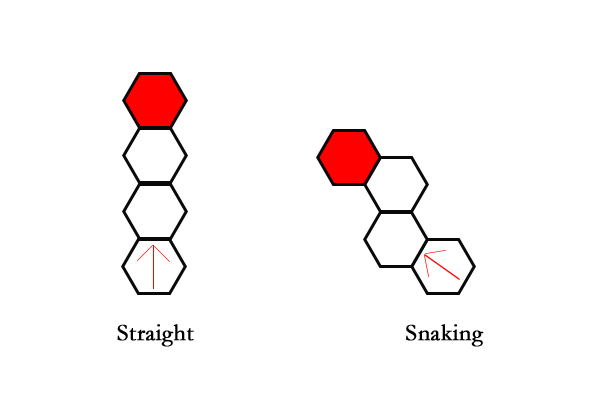
\includegraphics[scale=0.37]{misc/straight_snaking.png}}
\end{center}
Snaking can of course snake either left or right. And a snaking pattern may “curve” around obstacles and entities as long as it keeps its original pattern intact.\\
For charging-type attacks, the attack must be angled in the direction of the last move, or one hex adjacent to that direction.

\subsubsection{\emph{Sudden}}
\hypertarget{Sudden}{}
A \reftoit{Sudden} \emph{counterbeat} does not give the character the opportunity to commit a reaction.

\subsubsection{Unassigned Damage}
Damage that is not assigned to an \refto{HP} slot, deposited in a \reftoit{sink}, or placed on a \reftoit{Shield Up!} token is considered unassigned.

\subsubsection{Victory, Defeat, and Retreat}
After combat, refer to the encounter page. It will have specific instructions for whether the player won, retreated, or was defeated in the encounter. All conditions, even \emph{Static} ones, are removed at the end of an encounter, as is any unassigned damage.\\
The actual effects of each result are specific to their encounter.\\

\textbf{Victory:} Victory will usually reward the character with souls and perhaps some item or extra progression option. Neither \refto{HP} nor \refto{FP} are restored after an encounter, except for assigned Bleed tokens which are removed from their \refto{HP} slots.\\

\textbf{Defeat:} Defeat during an encounter will sometimes reduce the character’s \refto{HMN}. If the character was defeated with 0 \refto{HMN} remaining, they are likely to become Hollow.\\
Defeat also sometimes erases a character’s unspent souls, or robs the character of their \reftoit{Carried} items.\\
Some encounters can be repeated upon defeat. Other encounters might shunt the player into an alternative chapter route. Regardless, no scenario should be dependent on winning each and every encounter.\\

\textbf{Retreat:} In the event that victory seems unlikely, retreating is always encouraged when possible. If the character is located on a retreat tile during the \emph{beat}, and is not prevented from making a Move action; the player may elect to Retreat from the encounter as an action.

\vfill
\pagebreak

\subsection{Entity Concepts}
Both the character and enemies are referred to as “entities”. Entities is the term used when a gameplay concept applies equally to both parties. Likewise, entity sheet refers to both status and enemy sheets.\\
If a mechanic is specific to either the character or enemies, then that particular party will be named directly.

\subsubsection{Enemy Sheets}
Each enemy will need a miniature status sheet for itself: its enemy sheet. Index cards or scratch paper are useful for this purpose. Write any important stats such as Move on them for quick reference.\\
Draw a circle on the sheet for any \reftoit{sinks}. Also draw an \refto{HP} circle and write the \refto{HP} value in it (instead of drawing multiple slots). \\
When an encounter involves multiple identical enemies, there’s no need to write all of their information repeatedly. Just reproduce the \refto{HP} circle and any \reftoit{sinks}. Number the sheets and tokens, or use any other method, to keep track of who’s who.

\subsubsection{Enemy Types}
Enemies may have special types applied to them, such as \emph{Undead} or \emph{Intelligent}, which can give them special rules or make them obey certain mechanics. These rules should be explained in the scenario book and/or enemy description. A few of the default types are listed here.

\subsubsection*{Enemy Types Roster}
\textbf{Alert:} This entity is immune to the Backstab attack.\\

\textbf{Amphibious:} This entity ignores the normal effects of water tiles.\\

\textbf{Aquatic:} This entity ignores the normal effects of water tiles, and can only occupy tiles that are water.\\

\textbf{Floating/Flying:} This entity ignores hazard tiles and half-cover obstacles unless afflicted with Knockdown.\\

\textbf{Formation Fighter:} This entity forms some sort of formation with other entities, and the formation retains its own specific ruleset dictating their movement and attacks. Entities in a formation can normally attack past each other, and move as a single entity with one combined Turn.\\

\textbf{Great Foe:} In other words, a boss. This entity ignores all conditions inflicted by normal sources, except Blazing and Bleeding, and is immune to Backstab (but not Coup de Grâce).\\

\textbf{Hollowed:} This entity is insane and ignores the Charmed, Maddened, and Fear conditions.\\

\textbf{Intelligent:} This entity is either human or possesses a human-like intelligence. If the shortest route for an \emph{Intelligent} enemy’s movement would cause it to bunch up with other entities or otherwise not reach its intended target, it will take another, longer route to its target. \emph{Intelligent} enemies will also \emph{Drop!} and \emph{Roll!} away from the character if they are Blazing at the start of their \emph{counterbeat.}\\

\textbf{Large:} This entity occupies 2 tiles (head and tail) and ignores normal Knockback and Knockdown sources. For the purposes of movement and turning, the head tile is always moved first and the tail tile is filled-in behind the head, opposite its movement or attack direction.\\
There are some attacks that specifically originate from the head or tail, and use that tile to determine range. If an attack does not specify a head or tail tile, then it may originate from either.\\
If using coinage for entity tokens, the head and tail tile can easily be distinguished using those selfsame sides of the coins.\\

\textbf{Mounted:} This enemy rides something, and can be subjected to the Dismounted condition. The actual effect of being Dismounted is specific to each enemy.\\

\textbf{Undead:} This entity is \emph{Undead}, and is subject to certain attacks or effects that only affect the \emph{Undead.} Unless stated otherwise in the enemy’s description, an \emph{Undead} enemy is not affected by Bleed or Dark damage, nor subject to the Charmed, Bleeding, Maddened, or Fear conditions.\\

This is only a small selection of enemy types.

\subsubsection{Resolving Enemy Behavior}
Because \emph{Fires Far Away: A Solitaire Journey} does not have a human gamemaster, a large part of the system is dedicated to determining enemy behavior. When determining how an enemy behaves during its Turn, adhere to the following guidelines:\\

\textbf{1 -- The Encounter Roll:} The first step the player takes in determining the active enemy’s behavior is making its encounter roll. See the Encounter Resolution section for details.\\
Some encounter rolls may list out their instructions in plaintext if they’re particularly complicated, but normally they’ll just list the attack(s).\\
If there are multiple encounter tables, resolve their rolls in alphabetical order unless otherwise instructed.\\

\textbf{2 -- Conditional Behavior:} 
Some encounter rolls will provide conditional behavior for the active enemy. This allows enemies to perform alternative maneuvers when they can’t resolve an attack. This conditional behavior only hinges on whether the enemy is within range for the attack, not whether the attack will actually damage its target. An encounter roll’s conditional behaviors are resolved in alphabetical order (\textbf{A}, \textbf{B}, \textbf{C}, etc). The last listed behavior is the “default behavior” and is resolved even if the enemy cannot land its attack.\\

\textbf{3 -- Move:} Enemies cannot use their Move value unless the encounter roll specifically allows for it. When an encounter roll dictates a Move, enemies will normally move up to their maximum Move value towards the character using the shortest logical route to the nearest free hex. Some enemies may prefer to keep their distance from the character, which will be clearly dictated in the number of hexes such as “keeps 1 tile distance”. These enemies may also Move away from the character to maintain their preferred distance.\\
If the enemy cannot resolve a conditional behavior’s attack, it also cannot use that behavior’s Move (if any). The exception to this rule is if the enemy cannot resolve the last-listed behavior’s attack. In that case, resolve any Move regardless.\\
Enemies will normally skirt hazard tiles during movement, unless crossing hazard tiles is the only way of reaching the character.\\
If an enemy cannot reach the character, or there are no free adjacent tiles, it should move as close as possible using the shortest logical route, even if it needs to bunch up behind other entities.\\ 
Entities occupy their hexes entirely, meaning other entities cannot cross through them during a Move. The sole exception to this is knocked down entities.\\
Lastly, an enemy’s Move is cognizant of their encounter roll’s attack. So an enemy committing Move ahead of a ranged attack will move into range for that attack. This means that enemies will shoot across hazards instead of taking the long way around them.\\

\textbf{4 -- Attacking:} Refer to the enemy’s listed attacks for details on damage, modifiers, type, range, and any extra movement allowance.\\
If the enemy is out of range for an attack due to the character committing a reaction (such as Juke or \reftoit{Dodge!}), then the entity shall be treated as if it committed the attack anyway. The active enemy’s attempted behavior is never affected by a reaction.\\
Some attacks allow the active enemy to Move. This implicit Move is always available to the active enemy, regardless of whether they moved beforehand. If an enemy repeatedly commits an attack with an implicit Move, it gets to use the listed Move before each attack.\\

\textbf{5 -- Special Conditions:} Some enemies have special reactions to conditions like being knocked down. Refer to the enemy’s description page. This special behavior will be listed with the enemy’s other types, if any.\\

The result of this system is that enemy behavior is semi-predictable. The player can look at an encounter table and determine the exact moves its enemy might make (and tailor their Turn accordingly). However, the actual behavior of the enemy is still left to the roll.

\begin{tcolorbox}
\textbf{Note:} When in doubt, remember that this system is attempting to replicate intelligent human behavior for (most) enemies. If some behavior feels nonsensical, it probably is.
\end{tcolorbox}

\vfill
\pagebreak

\subsection{Equipment \& Attunement\newline Concepts}

\subsubsection{Attunements}
Attunements are spells and abilities that cost \refto{FP} tokens to use. Each attunement must be equipped in a number of \refto{POTs} equal to its Intensity. The character always has access to all of their known attunements during a \reftoit{short reprieve}. Using an attunement during a \reftoit{short reprieve} will still cost \refto{FP} tokens that cannot be restored during that same \reftoit{short reprieve}.\\
Attunements can only be re-assigned during a \reftoit{short reprieve}.\\
The method for learning attunements depends on the scenario, but is usually done through interacting with events or non-player characters.

\subsubsection{Broken Equipment}
Broken equipment is no longer usable. This includes whatever bonuses or special effects that equipment normally allows. Broken weapons cannot attack, broken shields cannot use \reftoit{Shield Up!}, broken rings provide no boons, broken catalysts cannot Cast, and so on and so forth. This equipment can be repaired during a \emph{short reprieve.}

\subsubsection{Catalysts}
In order to activate an attunement, the caster must equip a catalyst that allows for that attunement type. This catalyst’s Power assists in determining the quality of that sorcery, hex, miracle, or pyromancy. Guts-type attunements do not require a catalyst.

\subsubsection{\emph{Carried}}
\hypertarget{Carried}{}\hypertarget{carried}{}\hypertarget{carry}{}
The character can \reftoit{carry} additional items and pieces of equipment, but cannot access them during an encounter. They’re assumed to be kept in a pack, or stuffed under an armpit, or something. These \reftoit{Carried} items are noted on the record sheet. This mechanic is intended not only for hauling gear destined for the stash, but for holding onto just-in-case items as well--\reftoit{Carried} items and equipment can still be freely used or equipped outside of encounters.\\
The character has 8 \reftoit{Carried} slots.\\
\reftoit{Carried} items do not contribute to a character’s \refto{ENC}, regardless of their weight stat.\\
Unassigned attunements do not occupy \reftoit{Carried} slots. Attunements are knowledge, and are instead written in the “known attunements” section of the record sheet.\\
Some items, such as important keys, are written as notes and do not need to be \reftoit{Carried}.

\subsubsection{Defense (Armor \& Outfits)}
Armor’s primary purpose is to increase the size of the \refto{P.DEF} \reftoit{sink} by its Defense stat, in order to encapsulate more Physical damage tokens per Round. Some armor may also increase the size of other \emph{sinks.} See the \reftoit{Shield Up!} section for shield Defense.

\subsubsection{Dual Wielding}
A weapon wielded in the off-hand has all of its weapon scaling grades reduced by one full letter. Flip one hand token upside down to represent the off-hand.

\subsubsection{Durability}
Some equipment has Durability \reftoit{sinks} which can be used to mitigate damage like Acid/Breaking. If equipment has no Durability remaining, and takes Acid/Breaking damage, it becomes Broken.

\subsubsection{\emph{Ephemeral}}
\hypertarget{Ephemeral}{}
\reftoit{Ephemeral} equipment is deleted from the character sheet at the end of the chapter in which it’s found. In addition, \reftoit{Ephemeral} items never regain their charges.

\subsubsection{Flasks}
Flasks are equipped in pouches like any other item. Flasks produce effects when the character drinks from them. However, drinking necessitates proper situational awareness, as it is a Double action. Drinking from a flask reduces its charges by 1.

\subsubsection{Free Hand}
Leaving a free hand open on the character sheet alters the Use Item \refto{SP} cost to 2, and the Drink \refto{SP} cost to a flat 5. Remove one hand token to represent this.

\subsubsection{Hand Slots}
The character has four hand slots for equipping weapons, shields, and catalysts. Use two tokens (representing the character’s two hands) to track what’s being equipped in either hand. The passive effects (and weight) of equipment in hand slots is always in-play, regardless of whether or not that equipment is actually equipped.

\subsubsection{Items}
Miscellaneous items are equipped in pouches, and used via the Use Item action. When an item is used, reduce its charges (if any) by 1. Items’ charges are refilled during \reftoit{short reprieves}, unless they are \reftoit{Ephemeral}.\\
If the character has multiple items of the same type, they must be equipped in separate pouches. They cannot have their charges combined.\\
Items can only be used during an encounter if they are equipped in a pouch, but \reftoit{Carried} items can be used freely outside of encounters.\\
To mark charges, either keep tokens on the character sheet or add tokens as charges are used; whichever method feels right.

\subsubsection{Missiles}
Missiles must be equipped in a quiver in order to be utilized by ranged weaponry. A quiver is an item that takes up a pouch slot.\\
While \emph{Fires Far Away: A Solitaire Journey} is stern, it is not meant to be cruel. There are no ammunition limits for missiles. However, some ranged weaponry such as crossbows must be loaded by committing an action.\\
Thrown weapons such as javelins or throwing knives are not listed as ranged weapons or missiles, but are equipped in pouches as consumable items.

\subsubsection{One-Handing Two-Handed Weapons}
A two-handed weapon can be wielded in one hand if the character has double the \refto{STR} requirement.

\subsubsection{Pouches}
Pouches determine how many items a character can equip for use during an encounter. Characters naturally have 4 pouches available.

\subsubsection{Rings}
The character can wear a maximum of 2 rings at a time. Each ring presents some type of boon listed under its effects.

\subsubsection{Two-Handing One-Handed Weapons}
When two-handing a one-handed weapon, its \refto{STR} requirement is divided by 2 \emph{rd}. This reduced \refto{STR} requirement does not affect the weapon’s scaling.

\subsubsection{Weapon Scaling \& Upgrades}
Almost all weaponry has minimum Primary Stat requirements, most commonly \refto{STR} and \refto{DEX}. The character’s requisite stats must be equal or greater to the requirement(s) in order to wield a weapon.\\
Weapon damage also scales with these stats according to their “weapon scaling grade”. Each scaling grade has a threshold score. A weapon’s damage increases by 1 for each Primary Stat that reaches a multiple of its threshold score over the initial requirement. \\
A weapon’s damage can scale a limited number of times per stat, determined by that stat’s grade. This is listed as “Max” on the table below.\\
A E-grade stat has a requirement, but never increases damage.\\
\setlength{\tabcolsep}{10pt}
\renewcommand{\arraystretch}{1.5}
\begin{center}
\begin{tabular}{ |c|c|c|c|c|c|c| }
\hline
\multicolumn{7}{|c|}{\textbf{Weapon Scaling Grades}}\\
\hline
\textbf{Grade} & S & A & B & C & D & E \\
\hline
\textbf{Threshold} & 2 & 4 & 6 & 8 & 10 & - \\ 
\hline
\textbf{Max} & 4 & 3 & 2 & 2 & 2 & - \\
\hline
\end{tabular}
\end{center}

\begin{tcolorbox}
\textbf{Example:} A weapon that requires 10 \refto{STR} and has a B scaling grade will gain 1 point of damage when the character reaches 16 \refto{STR}.\\
A weapon with an A grade in \refto{STR} and a B grade in \refto{DEX} can scale its damage a total of 5 times (3 from \refto{STR}, 2 from \refto{DEX}).
\end{tcolorbox}

\vfill
\pagebreak

\section{The Player Character}
The character is comprised of seven Primary Statistics, each in turn influencing a host of Distributary Values. While this system may appear overly crunchy when filling out the character sheet, it allows for low-drag combat since all the math is done in advance.\\

\subsection{Primary Statistics}
The average starting score for any Primary Stat is 7. The lower limit is 3, and there is no upper limit. Increasing Primary Stats is done through upgrading the character’s Soul (\refto{SL}) during a \reftoit{short reprieve}.\\

\textbf{Vitality (\makeref{VIT})} – Increases Health and natural defenses.\\
\textbf{Endurance (\makeref{END})} – Increases \reftoit{stamina pool} size, max equipment load, and Resistance.\\
\textbf{Strength (\makeref{STR})} – Unlocks some weapons and scales their damage.\\
\textbf{Dexterity (\makeref{DEX})} – Unlocks some weapons and scales their damage.\\
\textbf{Attunement (\makeref{ATT})} – Increases Fire Bonus and Defense; and available \refto{FP} and \refto{POTs}.\\
\textbf{Intelligence (\makeref{INT})} – Unlocks and scales some attunements, raises some bonuses and defenses, and influences some weapon scales.\\
\textbf{Faith (\makeref{FTH})} – Unlocks and scales some attunements, raises some bonuses and defenses, and influences some weapon scales.\\
\textbf{Humanity (\makeref{HMN})} – A statistic particular to each scenario that determines how human, sane, corporeal, etc the character is. Reduced by suffering defeat or committing certain actions.\\ Losing Humanity often leads to insanity or other undesirable effects. It is normally granted at key points in a scenario, such as defeating a strong encounter. It can be thought of as a sort of lives system.\\
\textbf{Soul (\makeref{SL})} – Effectively the character’s “level”. Upgrading \refto{SL} allows the player to increase 1 Primary Stat on their character. Each scenario will utilize some resource for upgrading \refto{SL} (usually souls) and each subsequent upgrade will require a greater expenditure of them.\\
Upgrading \refto{SL} typically costs \emph{\refto{SL}+1} souls for each advancement, where \refto{SL} is the character’s current Soul.

\vfill

\subsection{Distributary Values}
These values are not directly increased via Soul advancement, but are influenced by the Primary Stats.\\

\textbf{Health (\makeref{HP})} – When all \refto{HP} slots are filled with damage tokens, the character is defeated.
\begin{itemize}
\item The character has \refto{HP} slots equal to:\\
2 + \refto{VIT}/2 \emph{rd.}
\end{itemize}

\textbf{Focus (\makeref{FP})} – Spent to activate attunements.
\begin{itemize}
\item The character has \refto{FP} tokens equal to:\\
2 + \refto{ATT}/2 \emph{rd.}
\end{itemize}

\setlength{\tabcolsep}{11pt}
\renewcommand{\arraystretch}{1.2}

\textbf{Stamina (\makeref{SP})} – Determines the number of \refto{SP} dice in the character’s \reftoit{stamina pool}, based on their \refto{END} score. These \refto{SP} dice are spent to perform actions during an encounter.
\definecolor{Gray}{gray}{0.85}
\rowcolors{2}{}{Gray}
\begin{center}
\begin{tabular}{ |c|c| }
\hline
\textbf{END Score} & \textbf{\# SP Dice}\\
\hline
1-10 & 4\\
\hline
11-15 & 5\\
\hline
16-20 & 6\\
\hline
21-25 & 7\\
\hline
26-30 & 8\\
\hline
31-35 & 9\\
\hline
36-40 & 10\\
\hline
41-45 & 11\\
\hline
46+ & 12\\
\hline
\end{tabular}
\end{center}

\textbf{Potential (\makeref{POT}/\makeref{POTs})} – The number of attunements a character can prepare simultaneously. This is represented via \refto{POTs}: slots that can be written-in with a spell or ability. Some attunements occupy multiple \refto{POTs}.
\begin{itemize}
\item At 7 \refto{ATT}, the first \refto{POT} is unlocked. Then for every 3 \refto{ATT} after 7 (10,13,16…) an additional \refto{POT} is granted.
\end{itemize}

\textbf{Equip Load (\makeref{EQP})} – Determines how much \refto{ENC} affects the character’s ability to use \reftoit{Dodge!}
\begin{itemize}
\item \refto{EQP} is equal to \refto{END} - 2.
\end{itemize}

\setlength{\tabcolsep}{6pt}
\renewcommand{\arraystretch}{1.5}

\columnbreak

\textbf{Encumbrance (\makeref{ENC})} – The total weight of all worn equipment. Most importantly, it determines the \reftoit{Dodge!} reaction, as well as some other actions like Vault, Juke, and Sprint. It also determines a character’s maximum Move value.

\rowcolors{2}{}{Gray}
\begin{center}
\begin{tabular}{ |c|c| }
\hline
\textbf{ENC vs EQP} & \textbf{\reftoit{Dodge!}}\\
\hline
ENC < EQP/2 \emph{rd} & 2 SP.  Move 1.\\
\hline
EQP/2 \emph{rd} <= ENC <= EQP & 3 SP. Move 1.\\
\hline
EQP < ENC < EQP*2 & 4 SP. No move.\\
\hline
EQP*2 <= ENC & No \reftoit{Dodge!}\\ 
\hline
\end{tabular}
\end{center}

\subsubsection{Bonuses}
Various bonuses to the \refto{PWR} of attunements, also raises defenses of that type.\\

\textbf{Magic Bonus (\makeref{MB})} – Influences the effectiveness of sorcery and \refto{M.DEF}.
\begin{itemize}
\item First \refto{MB} is gained at 10 \refto{INT}
\item Increases by 1 per 6 \refto{INT} over 10
\end{itemize}

\textbf{Fire Bonus (\makeref{FB})} – Influences the effectiveness of pyromancy and \refto{F.DEF}.
\begin{itemize}
\item First \refto{FB} is gained at 12 \refto{ATT}
\item Increases by 1 per 8 \refto{ATT} over 12
\end{itemize}

\textbf{Dark Bonus (\makeref{DB})} – Influences the effectiveness of witchery and \refto{D.DEF}.
\begin{itemize}
\item First \refto{DB} is gained at 8 \refto{INT} and 8 \refto{FTH}
\item Increases by 1 per 4 \refto{INT} or \refto{FTH} (whichever stat is the lowest) over 8
\end{itemize}
\begin{tcolorbox}
\textbf{Example:} 10 \refto{INT}, 8 \refto{FTH} would give 1 \refto{DB}.\newline 20 \refto{INT}, 8 \refto{FTH} would still give 1 \refto{DB}.
\end{tcolorbox}
\ \\
\textbf{Light Bonus (\makeref{LB})} – Influences the effectiveness of miracles and \refto{L.DEF}.
\begin{itemize}
\item First \refto{LB} is gained at 10 \refto{FTH}
\item Increases by 1 per 6 \refto{FTH} over 10
\end{itemize}

\vspace*{\fill}
\columnbreak

\subsubsection{Defenses}
Each Defense gives the character a \reftoit{sink} on their character sheet, where they can place incoming damage tokens instead of assigning them to \refto{HP} slots. Some \reftoit{sinks} can also mitigate conditions. These \reftoit{sinks} are cleared at the end of each Round.\\

\textbf{Physical Defense (\makeref{P.DEF})} – Base defenses against Crush, Slash and Pierce damage types.
\begin{itemize}
\item All three Physical damage types share this \reftoit{sink}
\item Increases naturally by 1 at 12 \refto{VIT}, and for every 8 \refto{VIT} over 12
\end{itemize}

\textbf{Magic Defense (\makeref{M.DEF})} – Defenses against Magic and \reftoit{Magical} Crush, Slash, and Pierce damage.
\begin{itemize}
\item Increases naturally by 1 per \refto{MB}
\end{itemize}

\textbf{Fire Defense (\makeref{F.DEF})} – Defenses against Burn damage.
\begin{itemize}
\item Increases naturally by 1 per \refto{FB}
\end{itemize}

\textbf{Dark Defense (\makeref{D.DEF})} – Defenses against Withering and Dark damage.
\begin{itemize}
\item Increases naturally by 1 per \refto{DB}
\end{itemize}

\textbf{Light Defense (\makeref{L.DEF})} – Defenses against Smite damage.
\begin{itemize}
\item Increases naturally by 1 per \refto{LB}
\end{itemize}

\textbf{Resistance (\makeref{RES})} – Defenses against the Disoriented and Stagger conditions; and Poison, Toxic, and Bleed damage (but not the Bleeding condition).
\begin{itemize}
\item Increases naturally by 1 per 12 \refto{END}, and for every 8 \refto{END} over 12
\end{itemize}

\textbf{Poise (\makeref{PS})} – Defenses against the Flinch, Dismounted, Knockback, and Knockdown conditions.
\begin{itemize}
\item Each tile of Knockback uses a \refto{PS} value
\item Cannot be increased naturally
\end{itemize}

\vspace*{\fill}
\columnbreak

\section{Encounter Gameplay}
Combat in \emph{Fires Far Away: A Solitaire Journey} is designed to be fast, deliberate, and mortal. Dice rolls set the stage for each Round of the encounter, but do not outright resolve its events. This allows the player more agency in combat, treating it like a puzzle rather than a roll off.\\
Each encounter takes place on the Hexagon-Tiled Map available at the end of this corebook. Setup instructions dictate where to initially place obstacles, hazards, enemies, and the character--utilizing the map’s hex coordinates.\\
Combat is resolved through a continuous loop of \emph{beats} and \emph{counterbeats}, also known as Turns, in which the player drives the initiative and the encounter responds in vicious kind.\\
The player acts in combat by committing \refto{SP} dice from the character’s \reftoit{stamina pool} to actions and reactions. The enemy does not use \refto{SP} dice, but instead rolls on the encounter table(s). Each encounter table contains entries for all possible dice rolls, which dictate enemy behavior and attacks.\\
Whenever the character depletes their \refto{SP} dice, the \reftoit{stamina pool} is re-rolled. This event also designates a Round, which is used in other mechanics.\\
Encounters reward speed and decisiveness. As Rounds accumulate, the encounter will grow more difficult. Whenever the \emph{round tally} strikes a given threshold, a \emph{doom event} will alter the encounter to the characters’ detriment.\\
When an entity’s \refto{HP} slots are filled with damage tokens, that entity is defeated and removed from the game. If the character suffers defeat in this manner, resolve the encounter’s instructions for defeat.\\
\begin{tcolorbox}
\textbf{Note:} Remember that a Round refers to a different gameplay mechanic than a Turn.\\
Turn refers to the series of successive \emph{beats} and \emph{counterbeats}.\\
Round refers to the encapsulating loop, marked by re-rolling the \reftoit{stamina pool}.
\end{tcolorbox}

\vspace*{\fill}
\columnbreak

\subsection{Encounter Setup}
To begin playing through an encounter:
\begin{enumerate}
\item Read the fluff section to understand the gist of the encounter
\item Grab a fresh copy of the Hexagon-Tiled Map, or erase the marks from an old sheet if it isn’t too cluttered
\item Refer to the encounter’s setup instructions. There should be an accompanying diagram of the map dictating what should go where
\item Begin by drawing any special tiles such as concealment or cover via symbols, cross-hatching, or different colors. Use \emph{light} shading so that the page can be used again
\item Grab an appropriate token or miniature for the character and place them on a valid starting location. Then place any initial entities
\item Grab an index card for each encounter table and write out all the rolls. Many encounter tables have identical result layouts, so cards can be re-used between encounters
\item Write the encounter’s enemy sheet(s) on index cards or scratch paper. Draw \refto{HP} circles and any \reftoit{sinks}, along with short-hand for other stats. See the Entity Concepts section for details
\item Lastly, remember what the victory conditions are for the encounter. Not every encounter revolves around defeating all of its enemies
\end{enumerate}
\pagebreak

\subsection{Encounter Resolution}
\subsubsection*{The Round}
An encounter begins with its first Round. Whenever the character would begin their Turn, but their \reftoit{stamina pool} is depleted, the encounter returns to the Round phase instead.\\
\textbf{Instructions:}
\begin{enumerate}
\item Increment the \emph{round tally} by 1 (starting at 1 for the very first Round)
\item Resolve any \emph{doom events} for the current \emph{round tally}
\item Unexhaust all results on the encounter table(s)
\item Clear all damage from shields and \reftoit{sinks}
\item Roll a number of dice according to the character’s \refto{SP} value and set them aside, numbers preserved, on the status sheet’s \reftoit{stamina pool}
\item Remove 1 token of each \emph{Time-Limited - Round} condition from all entity sheets
\end{enumerate}

\subsubsection*{The \emph{Beat}}
During the \emph{beat}, the player spends \refto{SP} dice to commit actions such as moving or attacking.\\
\textbf{Instructions:}
\begin{enumerate}
\item First, assign any trickling damage (such as Poison or Bleed) on the status sheet to \refto{HP} slots according to the damage instructions
\item The character must commit at least 1 action per \emph{beat}, with at least 1 \refto{SP} die spent per action. Each \refto{SP} die may only be spent on a single action, and their scores may not be split in any way. However, multiple \refto{SP} dice can be committed to a single action
\item The character may commit a maximum of 2 Simple actions per \emph{beat}; or 1 Simple action and 1 Dynamic action; or 1 Double action
\item In addition, the character may commit 1 Free action per \emph{beat}. This Free action does not count towards the character’s action minimum or action limit, and it may not be taken last
\item After all actions are resolved, remove 1 token of each \emph{Time-Limited - Turn} condition from the status sheet
\end{enumerate}

\subsubsection*{The \emph{Counterbeat}}
During the \emph{counterbeat}, the encounter orchestrates its entities and hazards according to the dice rolls on its encounter table(s).\\
\textbf{Instructions:}
\begin{enumerate}
\item Every \emph{beat} must be followed by a \emph{counterbeat}
\item First, assign any trickling damage (such as Poison or Bleed) on enemy sheets to their \refto{HP} circles according to the damage instructions
\item Roll on the encounter table(s) to determine the encounter roll(s). If a rolled entry is exhausted, resolve the next unexhausted entry to its right instead (looping if necessary)
\item Resolve the encounter roll for each enemy, in the order given by the encounter. The enemy resolving the encounter roll at any given time is known as the “active enemy”. Each active enemy resolves all its movement and attacks before moving onto the next enemy
\item Once an encounter roll is resolved, cover that entry with a token. That entry is now exhausted. If an encounter table contains duplicate entries, only the specific entry that was rolled becomes exhausted. Some entries may take multiple tokens to become exhausted; this will be specified in the table instructions
\item If all entries on an encounter table become exhausted, immediately un-exhaust the entire table
\item The player may commit \refto{SP} dice to a reaction after the active enemy resolves any Move, and before it resolves any attack(s)\\
\begin{tcolorbox}
\textbf{Note:} Encounter rolls with the \emph{sudden} tag will not give the player an opportunity for a reaction.
\end{tcolorbox}
\item The reaction is resolved before the active enemy’s attack(s). Therefore, reactions with movement may take the character out of the active enemy’s attack range. In that case, treat the attack as if it was committed anyway
\item Some attacks have an implicit Move value, which is part of the attack and therefore allows them to Move after the character’s reaction
\item If the active enemy commits multiple attacks, each attack is given its own reaction window. Reactions like \reftoit{Dodge!} only take effect for a single attack
\item The player may commit as many reactions per \emph{counterbeat} as they have \refto{SP} dice for, but only one reaction per attack
\begin{tcolorbox}
\textbf{Example:} The first enemy moves towards the character, who then reacts with \reftoit{Dodge!} That first enemy still attempts to resolve its attack, which misses thanks to \reftoit{Dodge!}\newline
A second enemy then moves towards the character, and attempts its own attack. The player has run out of \refto{SP} dice, and cannot commit a reaction, and so the second enemy lands its attack on the character.\newline
This same process would hold true for a single enemy attempting two, sequential attacks. Some enemies even have multiple attacks with Move values, allowing them to catch a character moving out of attack range during their reactions.
\end{tcolorbox}
\item After all enemy actions are resolved, remove 1 token of each \emph{Time-Limited - Turn} condition from all enemy sheets
\item Lastly, look at the character’s \emph{stamina pool.} If there are \refto{SP} dice remaining, the encounter goes into another \emph{beat.} However, if the \reftoit{stamina pool} is empty, return to the Round phase
\end{enumerate}
\begin{tcolorbox}
\textbf{Note:} For a quick reference sheet, see the Attached Sheets section at the end of this corebook.
\end{tcolorbox}
\end{multicols*}

\pagebreak
\subsection{Gameplay Example}
Here is a full playthrough of an example encounter. This should serve to further explain \emph{Fires Far Away: A Solitaire Journey’s} encounter system, including the setup process.
\subsubsection*{Example Encounter: The Hollowed Adventurer}
\begin{center}
\framebox{
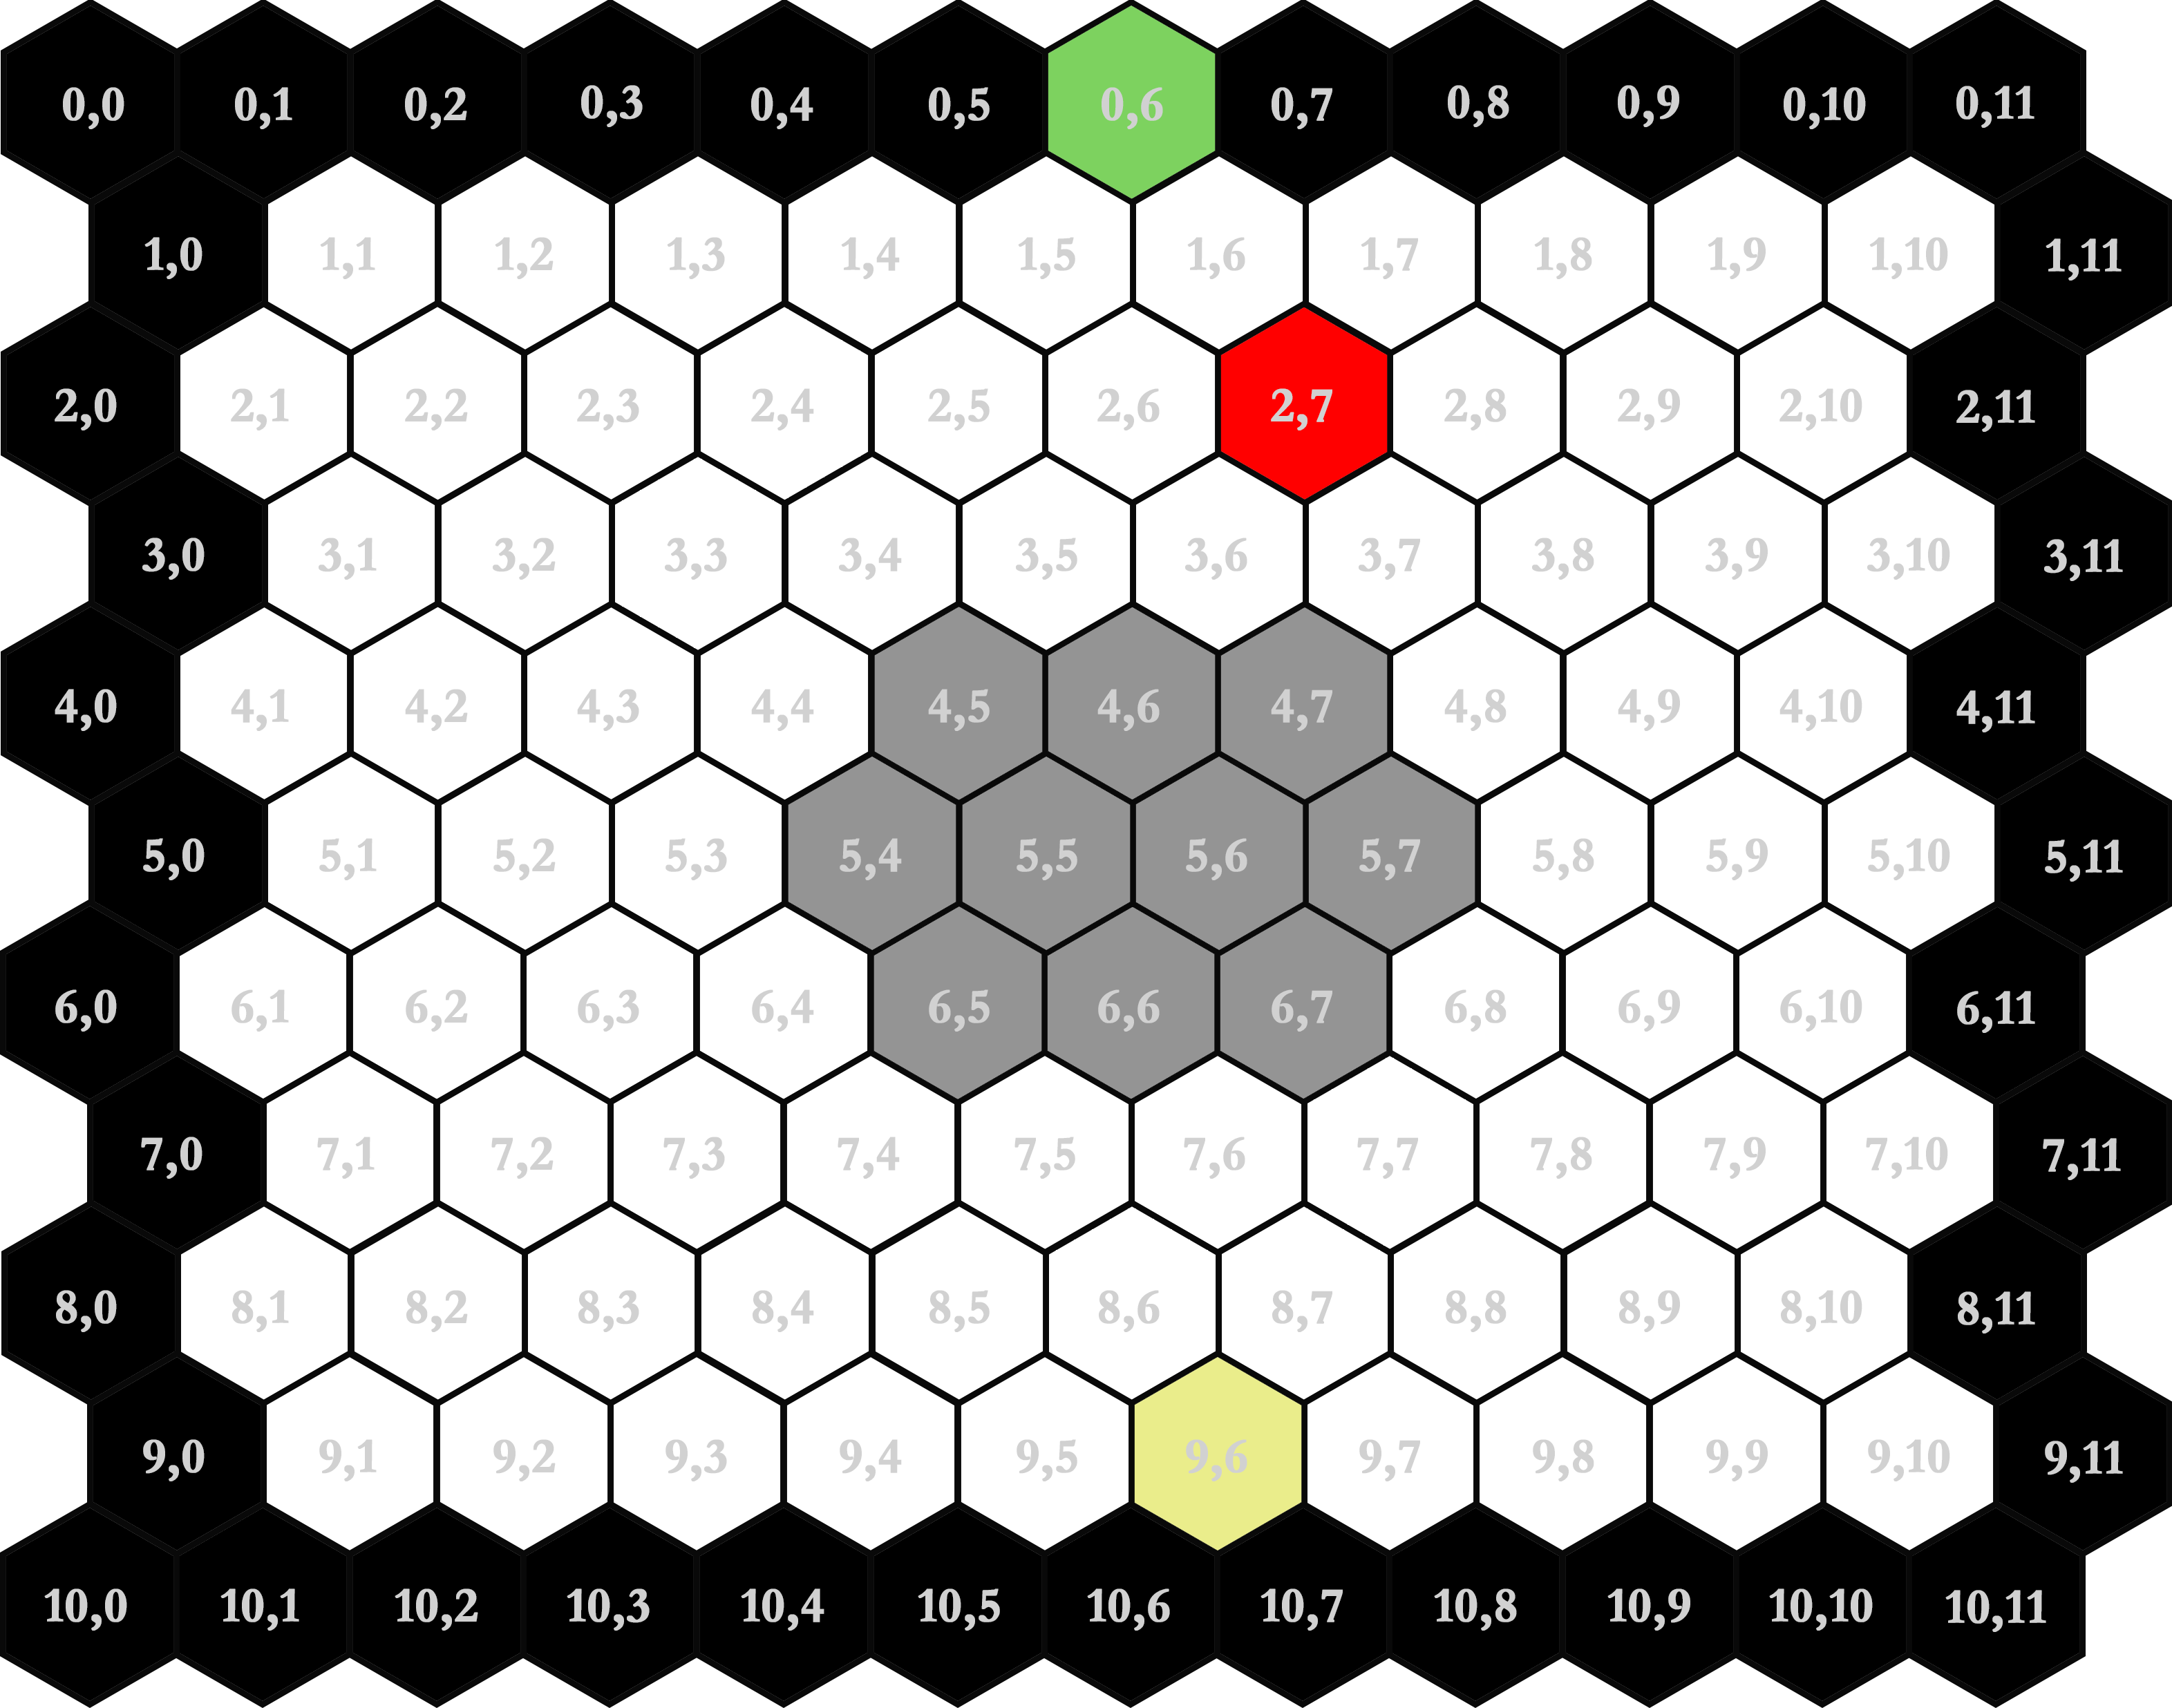
\includegraphics[width = 0.65\textwidth]{misc/example_map.png}
}
\end{center}
\subsubsection*{Setup Instructions}
\begin{itemize}
\item \textbf{Black:} Impassable Boundary.
\item \textbf{Goldenrod:} Character Start Location.
\item \textbf{Red:} Hollowed Adventurer Start Location.
\item \textbf{Grey:} Bottomless Pit. Any entity that enters this tile is defeated.
\item \textbf{Green:} Retreat Tile. Using the Retreat action on this tile ends the encounter.
\end{itemize}

\subsubsection*{Victory Condition}
Defeat the Hollowed Adventurer.

\subsubsection*{Doom Events}
\begin{itemize}
\item \textbf{Round 3:} Increase Hollowed Adventurer’s \refto{P.DEF} value by 1.
\item \textbf{Round 5:} Increase the damage of Hollowed Adventurer’s attacks by 1.
\end{itemize}

\pagebreak

\begin{multicols*}{2}
\subsubsection*{Setting up the Encounter}
First, the player grabs a copy of the Hexagon-Tiled Map. This copy was previously used for another encounter, so they carefully erase all the old marks and \emph{round tallies}. It’s best to draw lightly on the map for this reason.\\
Next, the player notes that this encounter has an impassable boundary. Filling in each perimeter hex would take too much time, and erasing it would be messy, so they draw an outline around the relevant tiles.\\
The retreat and bottomless pit tiles need symbols to distinguish them. The player decides on circles for the pit. For the retreat tile, an arrow pointing North seems appropriate.\\
Lastly, the player puts an American quarter-dollar on the character start location. As for the Hollowed Adventurer, they use a spent 9mm brass casing.\\
The encounter is now ready to play.

\subsubsection*{Studying the Enemy}
Before beginning the encounter, the player decides to look over their opponent. The hollowed adventurer has an enemy sheet, copied here:\\

\hrule
\subsubsection*{Hollowed Adventurer}
\refto{HP}: 13 \hspace*{2cm} \textbf{Move:} 4 \\
\refto{P.DEF}: 1 \\\\
\emph{Hollow:} This entity ignores the Charmed, Maddened, and Fear conditions.\\\\
\textbf{Attacks:}
\begin{itemize}
\item \emph{Shortsword} - Deal 2 Slash damage to an adjacent entity.
\item \emph{Wicked Slice} - Move 1. Deal 3 Slash damage. If any damage is assigned to an \refto{HP} slot, this attack also inflicts 1 Bleed damage.
\item \emph{Flurry} - Deal 2 Slash damage to an adjacent entity. Resolve this attack three times.
\end{itemize}
\hrule
\ \\ 
It’s not a particularly threatening opponent, but certainly an obstacle for a beginner character.\\

\columnbreak

The player also notes the encounter’s \emph{doom events}. On Round 3 the hollow will gain an extra point of \refto{P.DEF}, making them slightly harder to wound; and on Round 5 the hollow’s attacks begin to deal more damage. Like most encounters, this one rewards decisive action--it would be best to finish off the hollow before it gains these bonuses.

\subsubsection*{The Hero Enters}
Rather than including an entire character sheet, here are the relevant details for the player’s character:\\
\hrule
\subsubsection*{Genericus}
\refto{HP}: 6 \hspace*{2cm} \refto{P.DEF}: 2\\
\refto{SP}: 4 \hspace*{2.1cm} \textbf{\reftoit{Dodge!}:} 4 SP, No Move\\\\
\textbf{Equipment:}
\begin{itemize}
\item \emph{Arming Sword} - Costs 2 \refto{SP}. Deals 2 damage, inflicting either Slash or Pierce. Normally one-handed. Has the special attack: Lunge.
\item \emph{Spear} - Costs 2 \refto{SP}. Deals 2 Pierce damage. Has a range of 2 hexes. Normally one-handed. No special attacks.
\item \emph{Kite Shield} - Has 2 Defense, and 6 Stability. Retains 1 Durability \reftoit{sink}.
\item \emph{Sunlit Flask} - Removes up to 3 damage tokens from \refto{HP} slots.
\end{itemize}
\hrule
\ \\ \ \\
Genericus is a bog-standard, low-level fighter. He carries two weapons: the arming sword, and his spear. The sword is versatile, and allows him to Lunge an extra tile for attacks. The spear has no special attacks, and cannot perform the Slash moveset, but it has a range of 2 tiles and pairs well with a shield for Guarded Attacks.\\
Genericus also has a bit of a weight problem, making his \reftoit{Dodge!} action cost 4 \refto{SP} and afford no extra movement. But what he lacks in agility he makes up for with armor. His 2 \refto{P.DEF} will allow him to mitigate 2 Physical damage per Round, and ontop of that he has a kite shield for even further defenses.\\
Looking purely at stats, Genericus appears to be weaker than his opponent. However, he has one major advantage: his player. It’s Genericus’ fight to lose.
\end{multicols*}
\pagebreak

\subsubsection*{The Encounter Table}
\begin{tcolorbox}
\textbf{Roll:} 1D6
\begin{center}
\begin{tabular}{ L | L | L }
\multicolumn{1}{c|}{\textbf{1}} & 
\multicolumn{1}{c|}{\textbf{2-5}} & 
\multicolumn{1}{c}{\textbf{6}} \\
\textbf{A:} \emph{Flurry}\newline \textbf{B:} Move. \emph{Shortsword} &
Move. \emph{Shortsword}\newline \emph{This result is only exhausted after its third token} &
\emph{Sudden. Wicked Slice}
\end{tabular}
\end{center}
\end{tcolorbox}

\begin{multicols*}{2}
\subsubsection*{The Encounter Begins}
With setup complete and the two opponents’ statistics outlined on the previous page, it’s finally time to play the encounter. The encounter table has a common layout, so the player grabs an index card previously prepared with its rolls written out: 1, 2-5, and 6.
\subsubsection*{Round 1--}
Encounters always open on a Round. There isn’t much for the player to do besides mark the first \emph{round tally} in the map’s top right corner, and roll their \emph{stamina pool.} The 4 \refto{SP} dice come out: 2, 3, 3, 3.
\subsubsection*{\emph{Beat}}
The player looks over their opening moves. With this distance and no ranged weapon, Genericus lacks any opportunity to damage the hollow this Turn. But he still needs to take at least one action per \emph{beat.} The hollow has a Move value of 4, meaning it can get as close as \emph{6,8} or \emph{6,9} during the \emph{counterbeat.}\\
The player spends their 2-score dice to move Genericus to \emph{8,7}, and ends the Turn there. This will hopefully put him in range for a Light Attack next Turn.
\subsubsection*{\emph{Counterbeat}}
The player rolls 1D6 on the encounter table and checks the result: a 1. This would be bad if Genericus was in range for that \emph{Flurry} attack under the \textbf{A} behavior. However, since the enemy cannot resolve \textbf{A’s} attack they move onto \textbf{B}: a Move and a \emph{Shortsword} attack.\\
The hollow still can’t resolve its \emph{Shortsword} attack, but since it’s the lasted listed behavior it’s also the default. The hollow moves 4 hexes towards Genericus via the shortest logical route, landing on \emph{6,8}. The player then covers the encounter table’s 1 result with a coin, marking it as exhausted, and ends the Turn.
\subsubsection*{\emph{Beat}}
As predicted, Genericus is now within range--with his arming sword in one hand and the kite shield in his other. He could also use a Free action to switch to the spear, or even two-hand the sword, but the player has other plans.\\
They spend one of their 3-score dice to commit Light Attack, using its implicit Move to send Genericus forward to \emph{7,7}. This attack deals 2 Slash damage. One of these Physical damage tokens ends up in the hollow’s \refto{P.DEF} \reftoit{sink}; the other token reduces it to 12 \refto{HP}.\\
But the Turn isn’t over yet. That attack was a Dynamic action--Genericus can still perform a Simple action. The player decides to commit \reftoit{Shield Up!}, spending another 3-score die.
\begin{center}
\framebox{
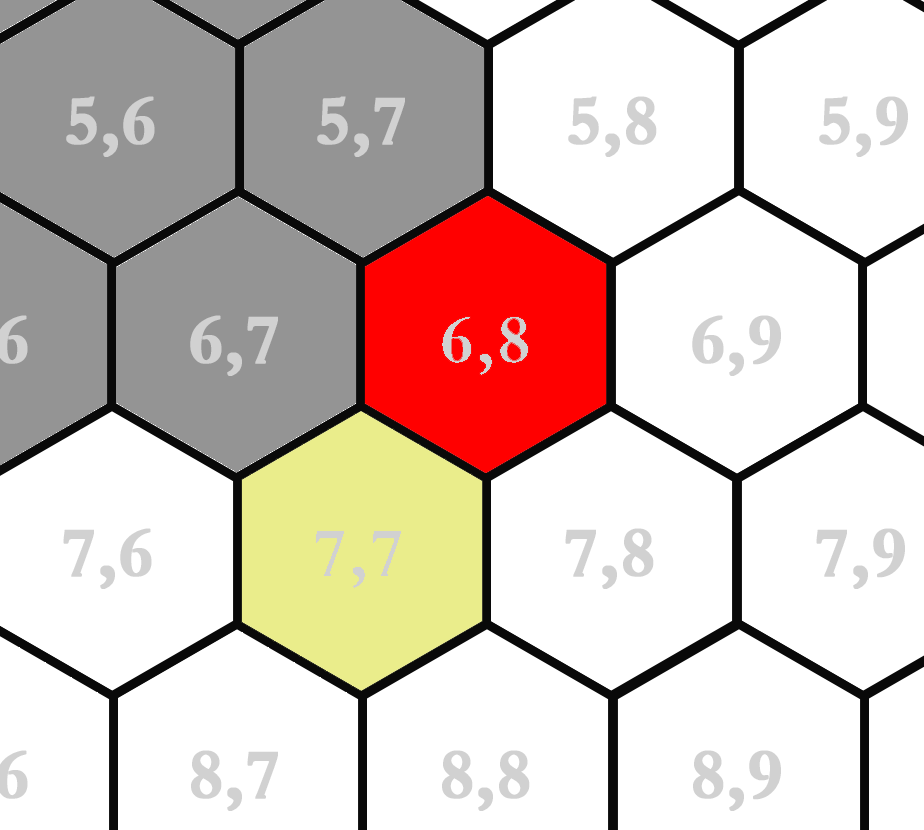
\includegraphics[width = 0.2\textwidth]{misc/example_map2.png}
}\\
\emph{Genericus and the hollow face off at the edge of a bottomless pit.}
\end{center}
\subsubsection*{\emph{Counterbeat}}
The player rolls on the encounter table again, coming up with a 6. Since this result is \emph{Sudden}, it prevents the player from committing a reaction--but thankfully, Genericus already has \reftoit{Shield Up!} ready.\\
\emph{Wicked Slice’s} first 2 Slash damage (the shield’s Defense value) is placed on \reftoit{Shield Up!} and the third token is assigned to \refto{P.DEF}. Because no damage was assigned to \refto{HP} slots, Genericus avoids taking any Bleed damage. The player exhausts the encounter table’s 6 result and ends the Turn.
\subsubsection*{\emph{Beat}}
The player decides to ditch the shield in favor of more damage, using the Free action Swap Equipment to two-hand the arming sword. Genericus only has one \refto{SP} die left, his last 3-score, and so the player spends it on a Heavy Attack. With a base damage of 2 and 1 \refto{SP} overspent, this attack will deal 3 Slash damage.\\
Since the hollow’s \refto{P.DEF} was already zeroed by the previous attack, this Heavy Attack reduces the hollow’s \refto{HP} from 12 to 9.
\begin{tcolorbox}
\textbf{Note:} The player could also use the arming sword to inflict Pierce instead of Slash damage, but it’s irrelevant in this situation.
\end{tcolorbox}
\subsubsection*{\emph{Counterbeat}}
The encounter roll comes up with another 1. Since the 1 result is already exhausted, the player resolves the next result to its right: 2-5. The hollow doesn’t need to Move since it’s already adjacent to Genericus, and so it goes right into the \emph{Shortsword} attack. Genericus lacks any \refto{SP} dice for a reaction, so he’s forced to eat both Slash damage tokens. The first is \reftoit{sunk} in his \refto{P.DEF}--the second reduces his \refto{HP} to 5.\\
Since the \reftoit{stamina pool} is now empty, instead of another \emph{beat} this encounter goes back to the Round phase.

\subsubsection*{Round 2--}
It is now Round 2, so the player marks a second tally in the top right corner. The encounter table is cleared of its tokens. Then, all damage tokens are removed from both \refto{P.DEF} \reftoit{sinks}, as well as \reftoit{Shield Up!} The rolls for the \reftoit{stamina pool} come out: 1,2,2,3.
\subsubsection*{\emph{Beat}}
The bad news this Round is that the player rolled poorly for \refto{SP} dice. But this does not render them totally impotent.\\
They commit the 3-score dice to another Heavy Attack, dealing 3 Slash damage. This eats through the hollow’s \refto{P.DEF} and drops it to 7 \refto{HP}.\\
The player then uses a Free action to re-equip the kite shield. Finally, they bring \reftoit{Shield Up!} back, spending a 2-score die.
\subsubsection*{\emph{Counterbeat}}
The encounter roll is a 3. The hollow performs another \emph{Shortsword} attack, landing 2 damage tokens on \reftoit{Shield Up!} Then a coin is placed on the 2-5 result. According to its instructions, this 2-5 result will not become exhausted until its third token.
\subsubsection*{\emph{Beat}}
With \reftoit{Shield Up!} stable, and the hollow at half health, the player decides to press their advantage. For 3 \refto{SP}, the player can commit Guarded Attack, which allows them to attack with Pierce damage and not lose their shield’s defenses. In order to meet the \refto{SP} requirement, the player commits both their remaining 1-score and 2-score dice. The hollow drops to 5 \refto{HP}.
\subsubsection*{\emph{Counterbeat}}
Disaster strikes when the player rolls a 1 on the encounter table. \emph{Flurry’s} first 4 damage go onto \reftoit{Shield Up!} but the fifth token inflicts \reftoit{Guard Break}. Since Genericus is already out of \refto{SP} dice, Flinch has no effect, but he still suffers Stun and loses 1 Durability on his kite shield. The sixth Slash damage token is \reftoit{sunk} in his \refto{P.DEF}.\\
Due to the empty \reftoit{stamina pool}, the encounter returns to the Round phase once again.

\subsubsection*{Round 3--}
With the coming of Round 3, things get even worse. A \emph{doom event} brings the hollow’s \refto{P.DEF} up to 2. Furthermore, Genericus is still Stunned and won’t be able to act on his first Turn. After clearing the encounter table, \reftoit{Shield Up!}, and both \reftoit{sinks}; the player’s \reftoit{stamina pool} rolls come out: 2,2,3,6.
\subsubsection*{\emph{Beat}}
Genericus cannot commit any actions due to Stun. The player removes the Stun condition token from his status sheet at the end of the Turn.
\subsubsection*{\emph{Counterbeat}}
The encounter roll comes up 4. The player could commit \reftoit{Dodge!} or even \reftoit{Shield Up!} again, but they want to save those \refto{SP} dice for ending this encounter ASAP. They deposit both damage tokens in \refto{P.DEF}.
\subsubsection*{\emph{Beat}}
The player commits one 2-score dice, and Moves to \emph{7,8}. Since Kick is also a Simple action, they could easily just send the hollow into the pit and end the encounter now. The player glances at the encounter results page (which is perfectly legal) and sees that kicking the hollow down the pit will deprive them of its souls and loot. To get anything out of this encounter, they must defeat the hollow the usual way.\\
The player decides on two-handing the arming sword again for another Heavy Attack, spending the 6-score die. This 4 Slash damage (the arming sword’s maximum) eats through the 2 \refto{P.DEF}. The hollow is now at 3 \refto{HP}.
\begin{center}
\framebox{
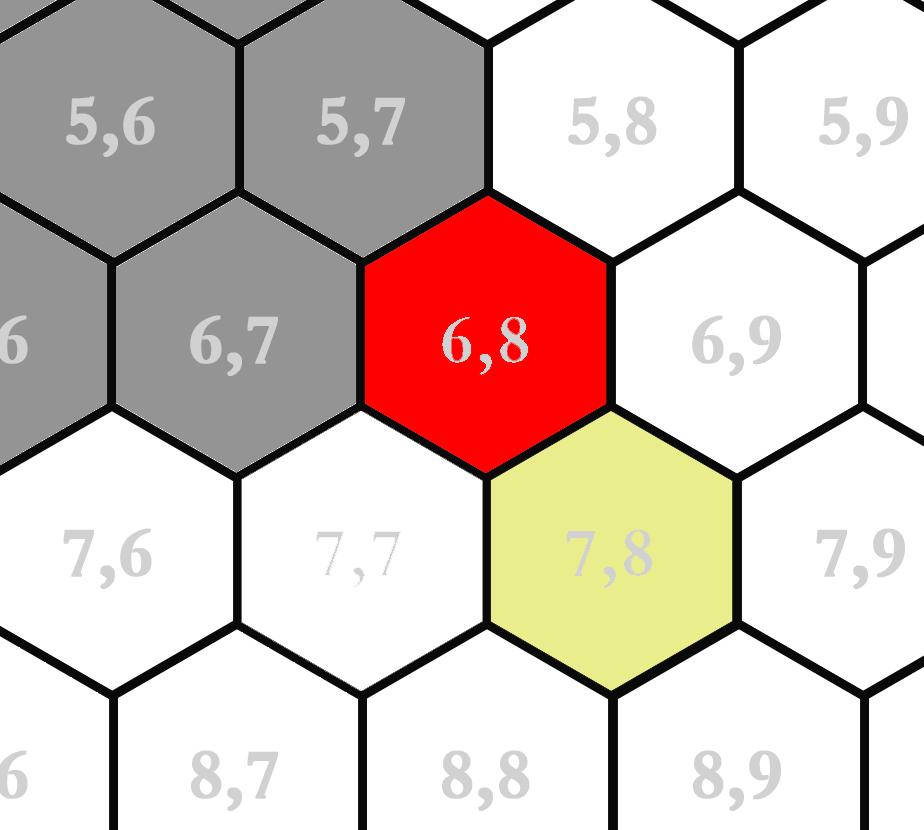
\includegraphics[width = 0.2\textwidth]{misc/example_map3.png}
}\\
\emph{Genericus considers sending the hollow over the edge.}
\end{center}
\subsubsection*{\emph{Counterbeat}}
The encounter table roll is another 1. With his \refto{P.DEF} gone, \emph{Flurry’s} 6 combined Slash damage would defeat Genericus. And since Genericus is two-handing his sword, committing \reftoit{Shield Up!} as a reaction isn’t an option. The player’s least odious solution is to commit \reftoit{Dodge!} for that first swing, and eat the remaining 4 damage. Since \reftoit{Dodge!} costs 4 \refto{SP}, this will require both the remaining 2-score and 3-score \refto{SP} dice, and the Round will end.\\
The player goes ahead and commits their remaining dice to saving Genericus. His \refto{HP} drops from 5 to 1.

\subsubsection*{Round 4--}
The player knows it’s do or die on Round 4. They mark the third \emph{round tally}, clear tokens from the usual places, and roll for their \reftoit{stamina pool}: 1,2,3,5.
\subsubsection*{\emph{Beat}}
Genericus will need to put out 5 damage to defeat the hollow. His highest possible damage output is 4 with a Heavy Attack, so this means a minimum of two attacks. But two separate encounter rolls, \emph{Flurry} and \emph{Wicked Slice} could easily defeat Genericus in a single \emph{counterbeat}--that’s two out of six rolls, a 33\% chance of defeat.\\
The player comes up with a simple strategy to ensure victory without having to Kick the hollow into the pit and lose out on the encounter rewards. First, they use a Free action to switch Genericus’ equipment to his spear and kite shield.\\
Next, the player spends the 2-score die to commit a Light Attack with the spear. This takes care of the hollow’s 2 \refto{P.DEF}.\\
Then the player commits the 3-score die to move Genericus to \emph{9,9}.
\begin{center}
\framebox{
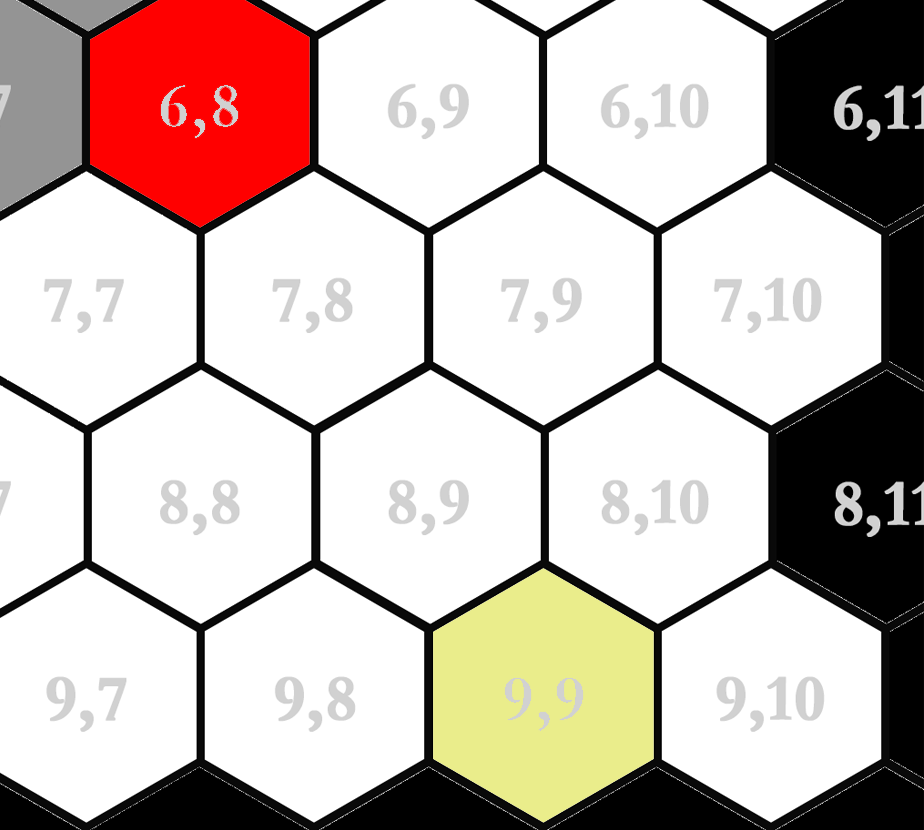
\includegraphics[width = 0.2\textwidth]{misc/example_map4.png}
}\\
\emph{Genericus enacts the plan.}
\end{center}
\subsubsection*{\emph{Counterbeat}}
The player rolls a 6 on the encounter table. This result may not have a Move, but the \emph{Wicked Slice} attack does have an implicit Move 1. The hollow moves to \emph{7,8}. This is exactly what the player was hoping for.
\subsubsection*{\emph{Beat}}
Now it’s time to finish the encounter. The player two-hands the spear and commits the 5-score die to a Heavy Attack (from 2 hexes away), dealing 4 Pierce damage and killing the hollow.

\subsubsection*{After the Battle}
The player checks the encounter’s rewards again: 20 souls, a shortsword, and some leather armor.\\
Despite winning the encounter, Genericus is not in great shape. Thankfully, the player can use a charge of the sunlit flask to regain 3 \refto{HP}, even outside of combat. But the kite shield is now at 0 Durability and at risk of breaking. Genericus could easily be looking at two or three more encounters before his next \reftoit{short reprieve}, where even one encounter might now prove fatal. In \emph{Fires Far Away: A Solitaire Journey}, small mistakes often end up compounding across a chapter.
\end{multicols*}

\pagebreak

\subsection{Actions \& Reactions}
\subsubsection*{Action \& Reaction Anatomy}
\begin{itemize}
\item \textbf{Action:} Self-explanatory.
\item \textbf{Type:} When the action can be committed. Either A – as an action, R – as a reaction, or E – in either case.
\item\textbf{SP:} The minimum \refto{SP} score that must be spent to commit the action. Wep refers to the attacking weapon’s stamina cost. Wep+n means the cost is increased by n. X means that the player must refer to the effect for specific instructions. F is a free action. 2D is a Double action, and takes up both actions for the \emph{beat}.
\item \textbf{Requires:} Any requirements for performing this action are entered in plain text. M refers to melee weapons, and C/S/P refers to required physical damage type(s) of the weapon, one of which must be applied. 1H/2H refers to one or two-handing the weapon. R refers to ranged weapons. LdR refers to ranged weapons that must be loaded before firing. Other requirements are self-explanatory. 
\item \textbf{Effect:} The effect that must be resolved after committing the action.
\end{itemize}

\renewcommand{\arraystretch}{1.5}
\definecolor{Gray}{gray}{0.85}
\rowcolors{1}{Gray}{}

\subsubsection{Simple Actions Roster}
Simple actions can be committed twice per \emph{beat}, or once in addition to a Dynamic action.\\

\begin{center}
\begin{tabularx}{\textwidth}{p{0.1\textwidth}p{0.08\textwidth}p{0.1\textwidth}p{0.2\textwidth}p{0.4\textwidth}}
\hline
\textbf{Action} & \textbf{Type} & \textbf{SP} & \textbf{Requires} & \textbf{Effect}\setcounter{rownum}{0}\\
\hline
\emph{Get Up!} & A & X & Knocked down & Remove Knockdown.\newline
Do not remove \reftoit{Shield Up!}\newline
If ENC<=EQP, \refto{SP} cost is 1D.\newline
If ENC<=EQP*2, \refto{SP} cost is 2.\newline
If ENC>EQP*2, \refto{SP} cost is 3\\
Juke & R & X & - & Move 1.\newline
Do not remove \reftoit{Shield Up!}\newline
If ENC<=EQP/2 \emph{rd}, \refto{SP} cost is 1D.\newline
If ENC<=EQP, \refto{SP} cost is 2.\newline
If ENC<=EQP*2, \refto{SP} cost is 3.\newline
If ENC>EQP*2, \refto{SP} cost is 4\\
Load & A & 2 & LdR\newline Missile available\newline No adjacent enemy & Select a missile from the quiver and make ready a loadable weapon. An already loaded weapon can have its ammunition swapped in this manner\\
Move & A & 1D+ & - & Move 1.\newline
Do not remove \reftoit{Shield Up!}\newline
May move an additional tile for each overspent \refto{SP}.\newline
If ENC>EQP, max Move is 5.\newline
If ENC>EQP*2, max Move is 4.\newline
If \reftoit{Shield Up!} is present on the status sheet, move a single hex for each 2 Move value\setcounter{rownum}{0}\\
\hline
\end{tabularx}
\end{center}

\pagebreak

\begin{center}
\begin{tabularx}{\textwidth}{p{0.1\textwidth}p{0.08\textwidth}p{0.1\textwidth}p{0.2\textwidth}p{0.4\textwidth}}
\hline
\rowcolor{white} \textbf{Action} & \textbf{Type} & \textbf{SP} & \textbf{Requires} & \textbf{Effect}\setcounter{rownum}{0}\\
\hline
\emph{Roll!} & E & 3 & Knocked down & Move 1.\newline
Remove Blazing\\
\reftoit{Shield Up!} & E & X & Shield Equipped & Add the \reftoit{Shield Up!} token to the status sheet.\newline
\refto{SP} cost is Def, where Def is the shield’s Defense value.\newline
This token is removed when committing any other action, unless that action specifically allows the character to keep their \reftoit{Shield Up!} token\\
Take Aim & A & 3 & - & The next non-attunement ranged attack or thrown item made this \emph{beat} gains 2 hexes in range.\newline
If the attack is made within the original weapon range, then the item or missile gains \reftoit{Unblockable}.\newline
If the attack is made within the original weapon range, the target does not possess \reftoit{Shield Up!}, then the attack gains 1 damage (as long as any damage existed prior)\\
Take Cover & R & 1D & Adjacent to half-cover & Any adjacent half-cover obstacles are treated as full-cover for one \emph{counterbeat}\\
Use Item & A & 3 & An item & Use any equipped item, reducing its charges by 1 and resolving its effects. Does not refer to flasks\\
\hline
\end{tabularx}
\end{center}

\pagebreak

\subsubsection{Dynamic Actions Roster}
Dynamic actions that can only be committed once per \emph{beat}, in addition to one Simple action.\\
\begin{center}
\begin{tabularx}{\textwidth}{p{0.1\textwidth}p{0.08\textwidth}p{0.1\textwidth}p{0.2\textwidth}p{0.4\textwidth}}
\hline
\textbf{Action} & \textbf{Type} & \textbf{SP} & \textbf{Requires} & \textbf{Effect}\setcounter{rownum}{0}\\
\hline
Cast & X & X & Catalyst & Cast an attunement using the equipped catalyst. \refto{PWR} is the character’s attunement type Bonus and catalyst’s Power combined.\newline See attunement details for \refto{SP} and \refto{FP} cost.\newline Only attunements tagged as reactions may be cast as such\\
\emph{Dive!} & E & 2 & - & Move 3.\newline
Place an \reftoit{Inevitable} Knockdown token on the status sheet\\
\emph{Dodge!}\hypertarget{Dodge!}{} & R & X & ENC<=EQP*2 & Refer to the character’s \refto{ENC} score for \refto{SP} cost and optional movement.\newline
Take no damage or conditions from the active enemy’s current attack unless it is \reftoit{Undodgeable}, \reftoit{Inevitable}, or \reftoit{Lock-On}\\
Drink & A & 2D & Flask with charges & Drink from an equipped flask, reducing its charges by 1 and resolving its effects\\
Gasp\newline \& Pant & A & - & - & Remove all remaining \refto{SP} Dice from the \reftoit{stamina pool}.\newline This is not a Free action\\
Retreat & A & 1D & Standing on a retreat tile, and able to Move & Resolve the encounter’s Retreat result\\
Sprint & A & 2D & ENC<EQP*2 & Move 6\\
\emph{Struggle!}\hypertarget{Struggle!}{} & A & 2D & - & Some conditions, such as Frozen, can only be removed by struggling. Remove 1 such condition token per use of \reftoit{Struggle!}\\
Summon Guts & X & X & - & Activate a Guts attunement. See attunements details for \refto{SP} and \refto{FP} cost. Only attunements tagged as reactions can be used as such\\
Vault & A & X & ENC<EQP*2 & Move 2, ignoring the effects of a hazard or tile of half-cover.\newline
If ENC<EQP/2 \emph{rd}, \refto{SP} cost is 3.\newline
If ENC<EQP, \refto{SP} cost is 4.\newline
If ENC<EQP*2, \refto{SP} cost is 5\\
\hline
\end{tabularx}
\end{center}

\pagebreak

\subsubsection{Free Actions Roster}
One Free action can be committed during a \emph{beat} for no \refto{SP} cost. Only one Free action may be committed per \emph{beat}, however, and it may not be taken as the final action.\\
A Free action does not count toward a \emph{beat’s} action minimum or action limit.\\
\begin{center}
\begin{tabularx}{\textwidth}{p{0.1\textwidth}p{0.08\textwidth}p{0.1\textwidth}p{0.2\textwidth}p{0.4\textwidth}}
\hline
\rowcolor{white} \textbf{Action} & \textbf{Type} & \textbf{SP} & \textbf{Requires} & \textbf{Effect}\setcounter{rownum}{0}\\
\hline
\emph{Drop!} & A & F & - & Place an \reftoit{Inevitable} Knockdown token on the status sheet\\
Lower Shield & A & F & \emph{Shield Up!} & Remove \emph{Shield Up!}\\
Swap Equipment & A & F & - & Swap hand tokens to any combination of hand slots on the character sheet.\newline
Do not remove \reftoit{Shield Up!} if the same shield is still equipped.\newline
This action can be used to two-hand or free hand a single weapon.\newline
The character still retains the passive bonuses of all equipment in hand slots, including their weight, regardless of whether they’re currently held\\
\hline
\end{tabularx}
\end{center}

\pagebreak

\subsubsection{Default Attacks Roster}
All attacks are considered Dynamic actions unless stated otherwise. All weapons are capable of making the following attacks, provided they meet the requirements.\\
\begin{center}
\begin{tabularx}{\textwidth}{p{0.1\textwidth}p{0.08\textwidth}p{0.1\textwidth}p{0.2\textwidth}p{0.4\textwidth}}
\hline
\textbf{Action} & \textbf{Type} & \textbf{SP} & \textbf{Requires} & \textbf{Effect}\\
\hline
Attack, Double & A & Wep1+Wep2 & Dual wielding & Perform two attacks, one with each equipped weapon, as a single Dynamic action\\
Attack, Guarded & A & Wep+1 & 1H M (P) & Attack an enemy within weapon range.\newline Do not remove \reftoit{Shield Up!}\\
Attack, Light & A & Wep & 1H M & Attack an enemy within weapon range.\newline
May Move 1 before attacking, but only in the direction of the attack\\
Attack, Heavy & A & Wep+ & 2H M & Attack an enemy within weapon range.\newline Apply an extra point of damage for every overspent \refto{SP}.\newline
This attack may be overspent up to double the weapon’s damage. Extra score committed past this is wasted\\
Attack, Opportunistic & R & Wep*2 & M & Make an attack on the active enemy immediately after it enters within weapon range. This attack can only occur after a Move\\
Bash & A & Wep+1 & M (C) & Attack an enemy within weapon range.\newline If this attack assigns 2 damage to \refto{HP} slots, it also inflicts Stun\\
Batter & A & 2 & R or LdR & Inflict Knockback 1 on an adjacent enemy, using the equipped ranged weapon.\newline This is a Simple action\\
Charge & A & 1D+Wep+ & M & Move 2-3 in a straight or snaking line.\newline
After moving, perform a Heavy Attack on an enemy within weapon range (not including the score from the 1D).\newline
Does not require 2H for the Heavy Attack.\newline
This is a Double action\\
Cleave & A & Wep+1 & 2H M (S)\newline Damage greater than 2 & Attack two enemies that are adjacent to each other and both within weapon range\\
Coup\newline De Grâce & A & Wep*2 & M & Deal double \reftoit{Unsinkable} damage to an adjacent enemy that is knocked down and does not have \reftoit{Shield Up!}\\
Draw\newline and Fire & A & Wep & 2H R\newline Missile available\newline No adjacent enemy & Select a missile from the quiver and deal weapon + missile damage to an enemy within their combined range\\
\hline
\end{tabularx}
\end{center}

\pagebreak

\begin{center}
\begin{tabularx}{\textwidth}{p{0.1\textwidth}p{0.08\textwidth}p{0.1\textwidth}p{0.2\textwidth}p{0.4\textwidth}}
\hline
\textbf{Action} & \textbf{Type} & \textbf{SP} & \textbf{Requires} & \textbf{Effect}\setcounter{rownum}{0}\\
\hline
Kick & A & 3 & - & Inflict Knockback 1 on an adjacent enemy that is not knocked down, and remove any \reftoit{Shield Up!} token from that enemy.\newline
If target enemy is knocked down, inflict Stun on that enemy instead.\newline This is a Simple action\\
Overhead & A & Wep+2 & M (C) & Attack all hexes in a forward or snaking line within weapon range, ignoring any minimum range.\newline
If this attack assigns 2 damage to \refto{HP} slots, it also inflicts Knockdown\\
Parry & R & X & M & Spend a \refto{SP} die matching one die rolled on the encounter table. Cancel the active enemy’s melee attack and inflict Stun on that enemy. Do not remove this Stun token at the end of the current \emph{counterbeat.}\newline The active enemy must be controlled by the encounter table with the matched die.\newline Cannot be used on \reftoit{Unparryable} attacks\\
Shield Bash & A & 2 & Shield & Inflict Knockback 1 and the equipped shield’s damage on an adjacent enemy, and move into its originally occupied hex.\newline Do not remove \reftoit{Shield Up!}\\
Shield Ram & A & 4 & Shield & Move 1-2 in a straight or snaking line.\newline After moving, inflict Knockback 2 and the equipped shield’s damage on an adjacent enemy, and move into its originally occupied hex.\newline Do not remove \reftoit{Shield Up!}\\
Shoot & A & Wep & 2H LdR\newline Loaded LdR & Deal weapon + missile damage of loaded ammunition to an enemy within their combined range. This unloads the weapon\\
Spin & A & Wep+3 & 2H M (S,C) & Attack six adjacent hexes in a full-moon pattern\\
Spin, Dual & A & 2D & Dual wielding & Attack six adjacent hexes in a full-moon pattern with both equipped weapons, one after the other\\
Sweep & A & Wep+2 & 2H M (S,C) & Attack three adjacent hexes in a half-moon pattern\\
Thrust & A & Wep+1 & M (P) & Attack all hexes in a forward or snaking line within weapon range, ignoring any minimum range\\
\hline
\end{tabularx}
\end{center}

\pagebreak

\subsubsection{Special Attacks Roster}
All attacks are considered Dynamic actions. Actions in this category are only available to weapons that specifically list them as special attacks.\\
\begin{center}
\begin{tabularx}{\textwidth}{p{0.1\textwidth}p{0.08\textwidth}p{0.1\textwidth}p{0.2\textwidth}p{0.4\textwidth}}
\hline
\rowcolor{white} \textbf{Action} & \textbf{Type} & \textbf{SP} & \textbf{Requires} & \textbf{Effect}\setcounter{rownum}{0}\\
\hline
Backstab & A & 3 + Wep*2 & M (P)\newline ENC<EQP*2 & Deal double \reftoit{Unblockable} and \reftoit{Unparryable} damage, and inflicts Knockdown, on an adjacent enemy.\newline
Move the character to the hex on the opposite side of that enemy. If the character cannot reach that tile, then they may not commit this attack.\newline
This is a Double action\\
Critical Strike & A & X & - & Must spend 2D of equal score. Perform a Light Attack dealing double damage.\newline
Does not require 1H for the Light Attack.\newline Counts as a single Dynamic action\\
Cut & A & Wep & M (S) & Attack an enemy within weapon range. If this attack assigns any damage to \refto{HP} slots, it also inflicts Bleeding\\
Defeat Guard & A & Wep+1 & - & Attack an enemy within weapon range with \reftoit{Unblockable} and \reftoit{Unparryable} damage\\
Fend & R & Wep*2 & - & Functions the same as the Opportunistic Attack reaction. Move directly backwards 1 hex (from the attack direction) after resolving Fend’s attack\\
Flurry & A & 2D & 1H M & Perform 3 Light Attacks (without their implicit Move) on a single enemy within weapon range\\
Harry & A & Wep+1 & - & Attack an enemy within weapon range, and then Move 1 in any direction.\newline
May Move 1 before attacking in any direction\\
Light/Douse & A & 2 & Doused weapon & Lights or douses a weapon, such as a torch\\
Lunge & A & Wep+1 & M (P) & Move 2 in a straight or snaking line.\newline After moving, attack an enemy within weapon range for \reftoit{Unparryable} Pierce damage\\
Mordhau & A & X & 2H M & Commit any attack from the Crush moveset, dealing Crush with -1 to damage\\
Plant Pavise & A & 3 & - & Exhaust the Pavise Shield equipment and changes a non-special tile to a half-cover obstacle\\
\hline
\end{tabularx}
\end{center}

\pagebreak

\begin{center}
\begin{tabularx}{\textwidth}{p{0.1\textwidth}p{0.08\textwidth}p{0.1\textwidth}p{0.2\textwidth}p{0.4\textwidth}}
\hline
\textbf{Action} & \textbf{Type} & \textbf{SP} & \textbf{Requires} & \textbf{Effect}\\
\hline
Pull & A & Wep+1 & - & Attack any enemy within weapon range, and then move that enemy to an adjacent hex\\
Pull Pavise & A & 3 & - & Unexhaust the Pavise Shield equipment and removes its tile of half-cover\\
Pulverize & A & 5 & 2H M & Inflict 1 Breaking damage on an enemy within weapon range \\
Puncture & A & Wep*2 & M (P) & Attack an enemy within weapon range with \reftoit{Unsinkable} damage\\
Riposte & R & X & - & Functions the same as the Parry reaction, but inflicts an immediate double damage attack from \emph{any} equipped weapon instead of Stun\\
Set Aflame & A & Wep+2 & Lit weapon & Inflicts Blazing on an enemy within weapon range\\
Shieldbreak & A & Wep+1 & 2H M & Inflict double damage on an enemy within weapon range that has \reftoit{Shield Up!}\newline This damage may only be assigned to \reftoit{Shield Up!} and will not “bleed over” after a \reftoit{Guard Break}\\
Tinker & A & 2D & - & Can clear 1 Durability \reftoit{sink} from any equipment, and a maximum of 1 such \reftoit{sink} via this method. This may remove Broken\\
Wild Swing & A & Wep+4 & 2H M (S,C) & Move 1-2 in a straight or snaking line.\newline After moving, attack three adjacent hexes in a half-moon pattern. Inflict Knockback 1 and Knockdown on all enemies struck by this attack\\
\hline
\end{tabularx}
\end{center}

\pagebreak

\section{Armory}
The corebook armory contains a list of default equipment. However, this does not mean that this equipment is available in all scenarios.
\subsection{Weapons}
\subsubsection*{Weapon Anatomy}
\begin{itemize}
\item \textbf{Weapon:} Self-explanatory
\item \textbf{SP:} The \refto{SP} score required to attack with this weapon
\item \textbf{Dam:} Base damage, and types of damage available (X means all three: Slash, Crush, and Pierce)
\item \textbf{Wt:} Weight of the weapon (always in effect, regardless of whether it’s currently held)
\item \textbf{Hd:} Whether the weapon is one-handed or two-handed by default
\item \textbf{Rg:} The maximum range of the weapon in tiles
\item \textbf{Dur:} Durability \reftoit{sinks} on the weapon, if any
\item The requirements for each Primary Stat, followed by their scaling grade
\item \textbf{S.Attacks:} Any special attacks enabled for the weapon
\item Any additional notes on the weapon
\end{itemize}

\subsubsection*{Weapons Roster}
\begin{center}
\begin{tabularx}{\textwidth}{p{0.12\textwidth}p{0.023\textwidth}p{0.054\textwidth}p{0.024\textwidth}p{0.024\textwidth}p{0.03\textwidth}p{0.03\textwidth}p{0.12\textwidth}p{0.11\textwidth}p{0.23\textwidth}}
\hline
\rowcolor{white} \multicolumn{10}{l}{\textbf{Daggers \& Knives}}\\
\hline
\rowcolor{white} \textbf{Weapon} & \textbf{SP} & \textbf{Dam} & \textbf{Wt} & \textbf{Hd} & \textbf{Rg} & \textbf{Dur} & \textbf{Stat Reqs} & \textbf{S.Attacks} & \textbf{Notes}\\
\hline
Dagger & 1 & 1 P & 1 & 1H & 1 & - & STR - 3|D\newline DEX - 3|D & Backstab & Coup De Grâce \refto{SP} cost is reduced to Wep\\
Fighting Knife & 1 & 1 S,P & 1 & 1H & 1 & - & STR - 4|D\newline DEX - 6|B & Backstab, Lunge & Coup De Grâce \refto{SP} cost is reduced to Wep\\
Jambiya & 1 & 1 S,P & 1 & 1H & 1 & - & STR - 4|D\newline DEX - 6|B & Backstab, Flurry & Coup De Grâce \refto{SP} cost is reduced to Wep\\
Mail Breaker & 2 & 2 P & 2 & 1H & 1 & 1 & STR - 8|C\newline DEX - 6|D & Backstab, Puncture & Puncture \refto{SP} cost is reduced to Wep+1\\
Main-Gauche & 1 & 1 P & 1 & 1H & 1 & 1 & STR - 5|D\newline DEX - 10|B & N/A & Coup De Grâce \refto{SP} cost is reduced to Wep\newline Parry-like actions can use \refto{SP} dice 1 score higher than the target die (if this weapon is currently held)\\
Rondel\newline Dagger & 1 & 1 P & 1 & 1H & 1 & - & STR - 4|D\newline DEX - 6|B & Backstab, Puncture & Coup De Grâce \refto{SP} cost is reduced to Wep\\
\hline
\end{tabularx}
\end{center}

\pagebreak

\begin{center}
\begin{tabularx}{\textwidth}{p{0.12\textwidth}p{0.023\textwidth}p{0.054\textwidth}p{0.024\textwidth}p{0.024\textwidth}p{0.03\textwidth}p{0.03\textwidth}p{0.12\textwidth}p{0.11\textwidth}p{0.23\textwidth}}
\hline
\rowcolor{white} \textbf{Weapon} & \textbf{SP} & \textbf{Dam} & \textbf{Wt} & \textbf{Hd} & \textbf{Rg} & \textbf{Dur} & \textbf{Stat Reqs} & \textbf{S.Attacks} & \textbf{Notes}\\
\hline
Seax & 1 & 1 S,P & 1 & 1H & 1 & 1 & STR - 4|D\newline DEX - 6|B & Cut,\newline Lunge & Coup De Grâce \refto{SP} cost is reduced to Wep\\
Stiletto & 1 & 1 P & 1 & 1H & 1 & - & STR - 3|D\newline DEX - 9|B & Backstab, Lunge, Puncture & Coup De Grâce \refto{SP} cost is reduced to Wep\\
Tecpatl & 1 & 1 S,P & 1 & 1H & 1 & - & STR - 3|D\newline DEX - 3|D\newline FTH - 9|E & Backstab, Cut & Coup De Grâce \refto{SP} cost is reduced to Wep\newline If this weapon inflicts Bleeding, it also inflicts 1 Dark damage\\
\hline
\rowcolor{white} \multicolumn{10}{l}{\textbf{Swords}}\\
\hline
Arming Sword & 2 & 2 S,P & 2 & 1H & 1 & 1 & STR - 7|C\newline DEX - 7|C & Lunge & N/A\\
Bastard Sword & 2 & 2 S,P & 2 & 1H & 1 & 1 & STR - 7|C\newline DEX - 7|C & Mordhau & N/A\\
Broadsword & 2 & 2 S,P & 2 & 1H & 1 & 1 & STR - 7|C\newline DEX - 7|C & Cut & N/A\\
Claymore & 3 & 4 S,P & 3 & 2H & 1 & 2 & STR - 10|B\newline DEX - 7|C & Lunge & Pierce attacks are range 2\\
Épée & 2 & 2 P & 1 & 1H & 1 & - & STR - 7|C\newline DEX - 10|B & Lunge, Puncture & N/A\\
Falchion & 2 & 2 S & 2 & 1H & 1 & 1 & STR - 7|C\newline DEX - 7|C & Harry & N/A\\
Falx & 2 & 2 S & 2 & 1H & 1 & 1 & STR - 7|C\newline DEX - 6|D & Shieldbreak & N/A\\
Flamberg & 3 & 4 S,P & 3 & 2H & 1 & 2 & STR - 10|B\newline DEX - 7|C & Cut & Pierce attacks are range 2\\
Greatsword & 4 & 5 S,P & 4 & 2H & 2 & 2 & STR - 14|A\newline DEX - 6|D & Wild Swing, Mordhau & Can use the Overhead attack, dealing Slash instead of Crush damage\\
Katana & 2 & 3 S,P & 2 & 2H & 1 & 1 & STR - 7|C\newline DEX - 9|C & Backstab, Critical Strike & Deals -1 damage for Pierce attacks\\
Khopesh & 2 & 2 S & 2 & 1H & 1 & 1 & STR - 7|C\newline DEX - 7|C\newline FTH - 9|E & Cut & If this weapon inflicts Bleeding, it also inflicts 1 Dark damage\\
Longsword & 3 & 4 S,P & 3 & 2H & 1 & 2 & STR - 10|B\newline DEX - 7|C & Mordhau & Pierce attacks are range 2\\
\hline
\end{tabularx}
\end{center}

\pagebreak

\begin{center}
\begin{tabularx}{\textwidth}{p{0.12\textwidth}p{0.023\textwidth}p{0.054\textwidth}p{0.024\textwidth}p{0.024\textwidth}p{0.03\textwidth}p{0.03\textwidth}p{0.12\textwidth}p{0.11\textwidth}p{0.23\textwidth}}
\hline
\rowcolor{white} \textbf{Weapon} & \textbf{SP} & \textbf{Dam} & \textbf{Wt} & \textbf{Hd} & \textbf{Rg} & \textbf{Dur} & \textbf{Stat Reqs} & \textbf{S.Attacks} & \textbf{Notes}\\
\hline
Odachi & 3 & 4 S,P & 3 & 2H & 1 & 2 & STR - 10|B\newline DEX - 9|C & Critical Strike &  Pierce attacks are range 2\newline Deals -1 damage for Pierce attacks\\
Rapier & 2 & 2 S,P & 1 & 1H & 1 & - & STR - 6|D\newline DEX - 13|A & Flurry, Lunge, Riposte & Deals -1 damage for Slash attacks\\
Saber & 2 & 2 S,P & 2 & 1H & 1 & 1 & STR - 7|C\newline DEX - 10|B & Cut,\newline Fend & N/A\\
Scimitar & 2 & 2 S & 2 & 1H & 1 & 1 & STR - 7|C\newline DEX - 10|B & Flurry, Harry & N/A\\
Shortsword & 2 & 2 S,P & 2 & 1H & 1 & 1 & STR - 7|C\newline DEX - 7|C & Flurry & N/A\\
Shotel & 2 & 2 S & 2 & 1H & 1 & 1 & STR - 7|C\newline DEX - 10|B & Defeat Guard & N/A\\
Tuck & 2 & 2 P & 2 & 1H & 1 & 1 & STR - 8|C\newline DEX - 10|B & Fend, Lunge & When two-handed, becomes a range 2 weapon\\
Washing Pole & 4 & 5 S,P & 4 & 2H & 2 & 2 & STR - 13|A\newline DEX - 10|C & Critical Strike & Pierce attacks are range 3\newline Deals -1 damage for Pierce attacks\\
Zulfiqar & 3 & 3 S & 3 & 1H & 1 & 2 & STR - 10|B\newline DEX - 10|B & Cut,\newline Flurry & N/A\\
Zweihander & 4 & 5 S,P & 4 & 2H & 2 & 2 & STR - 14|A\newline DEX - 6|D & Lunge, Wild Swing & Can use the Overhead attack, dealing Slash instead of Crush damage\\
\hline
\rowcolor{white} \multicolumn{10}{l}{\textbf{Bludgeons}}\\
\hline
Blackjack & 1 & 1 C & 1 & 1H & 1 & - & STR - 4|D\newline DEX - 5|D & Backstab & Backstab deals Crush damage and inflicts Stun\\
Club & 1 & 1 C & 1 & 1H & 1 & - & STR - 5|D\newline DEX - 4|D & N/A & Cannot be Broken\\
Flail & 2 & 2 C & 1 & 1H & 1 & 1 & STR - 6|C\newline DEX - 9|C & Defeat Guard & Overhead deals +1 damage\\
Giant Club & 3 & 4 C & 3 & 2H & 1 & - & STR - 10|B\newline DEX - 4|D & Wild Swing & Cannot be Broken\\
Goedendag & 3 & 4 C,P & 3 & 2H & 1 & 2 & STR - 10|B\newline DEX - 4|D & N/A & Pierce attacks are range 2\\
Great Mace & 4 & 5 C & 4 & 2H & 2 & - & STR - 14|A\newline DEX - 4|D & Pulverize & Cannot be Broken\\
Mace & 3 & 3 C & 2 & 1H & 1 & - & STR - 9|B\newline DEX - 4|D & N/A & Cannot be Broken\\
\hline
\end{tabularx}
\end{center}

\pagebreak

\begin{center}
\begin{tabularx}{\textwidth}{p{0.12\textwidth}p{0.023\textwidth}p{0.054\textwidth}p{0.024\textwidth}p{0.024\textwidth}p{0.03\textwidth}p{0.03\textwidth}p{0.12\textwidth}p{0.11\textwidth}p{0.23\textwidth}}
\hline
\rowcolor{white} \textbf{Weapon} & \textbf{SP} & \textbf{Dam} & \textbf{Wt} & \textbf{Hd} & \textbf{Rg} & \textbf{Dur} & \textbf{Stat Reqs} & \textbf{S.Attacks} & \textbf{Notes}\\
\hline
Mallet & 3 & 4 C & 3 & 2H & 2 & - & STR - 10|B\newline DEX - 4|D & N/A & Cannot be Broken\newline Overhead \refto{SP} cost reduced to Wep+1\\
Maul & 4 & 5 C & 4 & 2H & 1 & - & STR - 13|A\newline DEX - 3|E & Shieldbreak, Wild Swing & Cannot be Broken\\
Morgenstern & 3 & 4 P & 3 & 2H & 2 & 2 & STR - 10|B\newline DEX - 4|D & N/A & Deals Pierce damage, but uses the Crush moveset\newline Overhead \refto{SP} cost reduced to Wep+1\\
Morning Star & 3 & 3 P & 2 & 1H & 1 & 2 & STR - 9|B\newline DEX - 4|D & N/A & Deals Pierce damage, but uses the Crush moveset\\
Polehammer & 3 & 4 C,P & 3 & 2H & 2 & 2 & STR - 10|B\newline DEX - 7|D & Puncture & May deal Pierce damage, but can only use the Crush moveset\\
Shillelagh & 1 & 1 P & 1 & 1H & 1 & - & STR - 5|D\newline DEX - 4|D & N/A & Cannot be Broken\newline Deals Pierce damage, but uses the Crush moveset\\
Two-Handed Flail & 3 & 4 C & 3 & 2H & 2 & 1 & STR - 9|B\newline DEX - 9|C & Defeat Guard & Overhead can only damage 1 enemy, and deals +1 damage\\
Warhammer & 3 & 3 C,P & 2 & 1H & 1 & 2 & STR - 10|B\newline DEX - 6|D & Critical Strike & May deal Pierce damage, but can only use the Crush moveset\\
War Pick & 2 & 2 P & 2 & 1H & 1 & 2 & STR - 8|C\newline DEX - 4|D & Puncture & Deals Pierce damage, but uses the Crush moveset\newline Puncture \refto{SP} cost is reduced to Wep+1\\
\hline
\rowcolor{white} \multicolumn{10}{l}{\textbf{Polearms}}\\
\hline
Bardiche & 3 & 4 S & 2 & 2H & 2 & 1 & STR - 11|B\newline DEX - 7|C & Cut & N/A\\
Billhook & 3 & 4 S,P & 2 & 2H & 2 & 1 & STR - 11|B\newline DEX - 8|C & Pull & If this weapon assigns 2 damage to \refto{HP} slots in a single attack, it also inflicts Dismounted\\
Doru & 3 & 3 P & 3 & 1H & 2-3 & 1 & STR - 9|C\newline DEX - 9|C & N/A & N/A\\
Glaive & 3 & 4 S,P & 2 & 2H & 2 & 1 & STR - 11|B\newline DEX - 8|C & Fend & N/A\\
\hline
\end{tabularx}
\end{center}

\pagebreak

\begin{center}
\begin{tabularx}{\textwidth}{p{0.12\textwidth}p{0.023\textwidth}p{0.054\textwidth}p{0.024\textwidth}p{0.024\textwidth}p{0.03\textwidth}p{0.03\textwidth}p{0.12\textwidth}p{0.11\textwidth}p{0.23\textwidth}}
\hline
\rowcolor{white} \textbf{Weapon} & \textbf{SP} & \textbf{Dam} & \textbf{Wt} & \textbf{Hd} & \textbf{Rg} & \textbf{Dur} & \textbf{Stat Reqs} & \textbf{S.Attacks} & \textbf{Notes}\\
\hline
Halberd & 4 & 5 S,P & 3 & 2H & 2 & 1 & STR - 13|A\newline DEX - 8|C & N/A & Sweep \refto{SP} cost is reduced to Wep+1\newline Spin \refto{SP} cost is reduced to Wep+2\\
Harpoon & 2 & 2 P & 1 & 1H & 2 & 1 & STR - 6|D\newline DEX - 7|C & N/A & All attacks have the effect of the Pull attack; cannot forgo using this effect\\
Pike & 4 & 5 P & 3 & 2H & 2-4 & 1 & STR - 14|A\newline DEX - 8|C & N/A & N/A\\
Spear & 2 & 2 P & 2 & 1H & 2 & 1 & STR - 7|C\newline DEX - 7|C & N/A & N/A\\
Trident & 3 & 4 P & 2 & 2H & 2 & 1 & STR - 9|C\newline DEX - 9|C & Puncture & N/A\\
Voulge & 3 & 4 S,P & 2 & 2H & 2 & 1 & STR - 10|B\newline DEX - 7|D & Shieldbreak & N/A\\
Quarterstaff & 1 & 2 C & 1 & 2H & 2 & - & STR - 6|C\newline DEX - 6|C & Riposte & Deals Crush damage, but may use the Pierce and Crush movesets (but not Thrust)\\
\hline
\rowcolor{white} \multicolumn{10}{l}{\textbf{Axes}}\\
\hline
Battle Axe & 3 & 3 S & 3 & 1H & 1 & 1 & STR - 10|B\newline DEX - 7|D & Shieldbreak & Cleave \refto{SP} cost reduced to Wep\\
Hatchet & 1 & 1 S & 1 & 1H & 1 & 1 & STR - 5|D\newline DEX - 5|D & N/A & N/A\\
Labrys & 3 & 3 S & 3 & 1H & 1 & 1 & STR - 10|B\newline DEX - 7|D & N/A & Sweep \refto{SP} cost reduced to Wep+1\newline Spin \refto{SP} cost reduced to Wep+2\\
Long Axe & 3 & 4 S & 3 & 2H & 2 & 2 & STR - 11|B\newline DEX - 6|D & Shieldbreak & N/A\\
Macuahuitl & 2 & 2 S & 1 & 1H & 1 & - & STR - 7|C\newline DEX - 7|C & Cut & Deals Slash damage, but uses the Crush moveset\\
Pollaxe & 4 & 5 X & 4 & 2H & 2 & 2 & STR - 15|A\newline DEX - 7|D & Pulverize, Shieldbreak & Deals -1 damage for Pierce and Crush attacks\\
Skeggox & 3 & 3 S & 3 & 1H & 1 & 1 & STR - 10|B\newline DEX - 7|D & Wild Swing & N/A\\
Tabar-Zin & 3 & 3 S,P & 3 & 1H & 1 & 1 & STR - 10|B\newline DEX - 7|D & Puncture, Shieldbreak & Deals -1 damage for Pierce attacks\\
\hline
\end{tabularx}
\end{center}

\pagebreak

\begin{center}
\begin{tabularx}{\textwidth}{p{0.12\textwidth}p{0.023\textwidth}p{0.054\textwidth}p{0.024\textwidth}p{0.024\textwidth}p{0.03\textwidth}p{0.03\textwidth}p{0.12\textwidth}p{0.11\textwidth}p{0.23\textwidth}}
\hline
\rowcolor{white} \textbf{Weapon} & \textbf{SP} & \textbf{Dam} & \textbf{Wt} & \textbf{Hd} & \textbf{Rg} & \textbf{Dur} & \textbf{Stat Reqs} & \textbf{S.Attacks} & \textbf{Notes}\\
\hline
War Axe & 4 & 5 S & 4 & 2H & 1 & 2 & STR - 13|A\newline DEX - 6|D & Shieldbreak, Wild Swing & N/A\\
\hline
\rowcolor{white} \multicolumn{10}{l}{\textbf{Ranged Weaponry}}\\
\hline
Arbalest & 1 & 3 & 3 & 2H & 9 & 1 & STR - 10|E\newline DEX - 8|C\newline INT - 7|E & N/A & Loadable ranged weapon\newline Damage type dependent on missile (uses bolts)\newline The Load action \refto{SP} cost is increased to 3\\
Hand\newline Crossbow & 1 & 1 & 1 & 1H & 5 & 1 & STR - 6|E\newline DEX - 7|C\newline INT - 6|E & N/A & Loadable ranged weapon\newline Damage type dependent on missile (uses bolts)\newline Can commit Shoot one-handed\\
Heavy\newline Crossbow & 1 & 2 & 3 & 2H & 7 & 1 & STR - 10|E\newline DEX - 8|C\newline INT - 6|E & N/A & Loadable ranged weapon\newline Damage type dependent on missile (uses bolts)\\
Light\newline Crossbow & 1 & 1 & 2 & 2H & 7 & 1 & STR - 8|E\newline DEX - 8|C\newline INT - 6|E & N/A & Loadable ranged weapon\newline Damage type dependent on missile (uses bolts)\\
Longbow & 3 & 2 & 2 & 2H & 2-8 & 1 & STR - 10|D\newline DEX - 9|B & N/A & Ranged weapon\newline Damage type dependent on missile (uses arrows)\\
Recurve Bow & 2 & 1 & 2 & 2H & 2-6 & 1 & STR - 7|D\newline DEX - 9|B & N/A & Ranged weapon\newline Damage type dependent on missile (uses arrows)\\
Short Bow & 2 & - & 1 & 2H & 2-5 & - & STR - 5|D\newline DEX - 6|C & N/A & Ranged weapon\newline Damage and damage type dependent on missile (uses arrows)\\
Sling & 1 & 1 C & 1 & 1H & 2-5 & - & STR - 4|D\newline DEX - 6|C & N/A & Ranged weapon\newline Does not require missiles or a quiver\newline Can commit Draw \& Fire one-handed\\
Staff Sling & 2 & 2 C & 2 & 2H & 2-8 & - & STR - 6|D\newline DEX - 7|C & N/A & Ranged weapon\newline Does not require missiles or a quiver\\
\hline
\end{tabularx}
\end{center}

\pagebreak

\begin{center}
\begin{tabularx}{\textwidth}{p{0.12\textwidth}p{0.023\textwidth}p{0.054\textwidth}p{0.024\textwidth}p{0.024\textwidth}p{0.03\textwidth}p{0.03\textwidth}p{0.12\textwidth}p{0.11\textwidth}p{0.23\textwidth}}
\hline
\rowcolor{white} \multicolumn{10}{l}{\textbf{Special Weapons}}\\
\hline
\rowcolor{white} \textbf{Weapon} & \textbf{SP} & \textbf{Dam} & \textbf{Wt} & \textbf{Hd} & \textbf{Rg} & \textbf{Dur} & \textbf{Stat Reqs} & \textbf{S.Attacks} & \textbf{Notes}\\
\hline
Blacksmith’s Hammer & 2 & 2 C & 1 & 1H & 1 & 1 & STR - 9|C\newline DEX - 4|E & Tinker & Cannot be Broken\\
Butcher’s Cleaver & 1 & 1 S & 1 & 1H & 1 & - & STR - 3|D\newline DEX - 3|D & Cut & Coup De Grâce \refto{SP} cost is reduced to Wep\\
Caestus & 2 & 2 C & 1 & 1H & 1 & - & STR - 5|D\newline DEX - 5|D & Flurry & If this weapon assigns 3 damage to \refto{HP} slots in a single attack, it also inflicts 1 Bleed\newline No 2H\\
Farming Scythe & 2 & 3 S & 3 & 2H & 2-3 & 1 & STR - 6|D\newline DEX - 4|E & Cut,\newline Pull & Sweep \refto{SP} cost is reduced to Wep+1\newline Spin \refto{SP} cost is reduced to Wep+2\\
Felling Axe & 2 & 3 S & 2 & 2H & 1 & 2 & STR - 6|D\newline DEX - 6|D & Shieldbreak & N/A\\
Fist & 2 & 1 C & - & 1H & 1 & - & N/A & Flurry & Cannot be Broken\newline Increases damage by 1 at 14 \refto{STR}/22 \refto{STR}\newline Used if nothing equipped\newline No 2H\\
Lantern & 2 & 2 C & 2 & 1H & 1 & - & N/A & Light/Douse & Counts as a light source when lit\newline Becomes doused if used to attack\\
Loose\newline Cobblestone & 1 & 1 C & - & 1H & 1 & - & STR - 3|D\newline DEX - 3|E & N/A & \reftoit{Ephemeral}\newline Cannot be Broken\newline No 2H\\
Katar & 2 & 2 P & 2 & 1H & 1 & 1 & STR - 7|C\newline DEX - 9|C & Backstab, Cut,\newline Lunge & No 2H\\
Man Catcher & 2 & 3 P & 3 & 2H & 2 & 1 & STR - 8|D\newline DEX - 7|E & Pull & If this weapon assigns any damage to an \refto{HP} slot in a single attack, it also inflicts Netted/Webbed and Dismounted, but becomes exhausted on the character sheet until Netted/Webbed is removed\\
Pickaxe & 2 & 2 P & 1 & 1H & 1 & 2 & STR - 8|D\newline DEX - 4|E & Puncture & Deals Pierce damage but uses the Crush moveset\\
\hline
\end{tabularx}
\end{center}

\pagebreak

\begin{center}
\begin{tabularx}{\textwidth}{p{0.12\textwidth}p{0.023\textwidth}p{0.054\textwidth}p{0.024\textwidth}p{0.024\textwidth}p{0.03\textwidth}p{0.03\textwidth}p{0.12\textwidth}p{0.11\textwidth}p{0.23\textwidth}}
\hline
\rowcolor{white} \textbf{Weapon} & \textbf{SP} & \textbf{Dam} & \textbf{Wt} & \textbf{Hd} & \textbf{Rg} & \textbf{Dur} & \textbf{Stat Reqs} & \textbf{S.Attacks} & \textbf{Notes}\setcounter{rownum}{0}\\
\hline
Sock Full of Rocks & 1 & 1 C & 1 & 1H & 1 & - & STR - 3|D\newline DEX - 4|D & Defeat Guard & \reftoit{Ephemeral}\newline Overhead deals +1 damage\\
Torch & 1 & 1 C & 1 & 1H & 1 & - & N/A & Light/Douse,\newline Set Aflame &  Must be lit to use Set Aflame\newline Counts as a light source when lit\\
Urumi & 2 & 2 S & 1 & 1H & 2-3 & 1 & STR - 4|E\newline DEX - 11|B & Cut,\newline Defeat Guard & If this weapon assigns any damage to \refto{HP} slots in a single attack, it also inflicts 1 Bleed\newline Cannot commit Parry or Coup De Grâce\\
Whip & 2 & 1 S & 1 & 1H & 2-3 & - & STR - 4|E\newline DEX - 8|C & Defeat Guard,\newline Pull & If this weapon assigns any damage to \refto{HP} slots in a single attack, it also inflicts 1 Bleed\newline Cannot commit Parry or Coup De Grâce\\
\hline
\rowcolor{white} \multicolumn{10}{l}{\textbf{Unique Weapons}}\\
\hline
Abyssal Greatsword & 4 & 5 S,P & 4 & 2H & 2 & 2 &  STR - 14|A\newline DEX - 8|C\newline INT - 10|B & Lunge, Wild Swing & Can use the Overhead attack, dealing Slash instead of Crush damage\newline Also deals 1 Dark damage; INT scaling increases this Dark damage, not damage\\
Ardent Spear & 2 & 2 P & 2 & 1H & 2 & 1 & STR - 10|B\newline DEX - 10|B & Lunge, Puncture & If this weapon assigns 2 damage to \refto{HP} slots in a single attack, commit a Free Light Attack (limit once per Turn)\\
Axe of\newline Hatred & 3 & 3 S & 3 & 1H & 1 & 2 & STR - 14|A\newline DEX - 7|D & Shieldbreak, Wild Swing & Add any damage assigned to \refto{HP} slots last \emph{counterbeat} as bonus Dark damage\\
Bandit’s Knife & 1 & 1 S,P & 1 & 1H & 1 & - & STR - 6|D\newline DEX - 11|A & Backstab, Cut,\newline Flurry & Coup De Grâce \refto{SP} cost is reduced to Wep\newline May activate “Slink” without attuning it, or learning the attunement\setcounter{rownum}{0}\\
\hline
\end{tabularx}
\end{center}

\pagebreak

\begin{center}
\begin{tabularx}{\textwidth}{p{0.12\textwidth}p{0.023\textwidth}p{0.054\textwidth}p{0.024\textwidth}p{0.024\textwidth}p{0.03\textwidth}p{0.03\textwidth}p{0.12\textwidth}p{0.11\textwidth}p{0.23\textwidth}}
\hline
\rowcolor{white} \textbf{Weapon} & \textbf{SP} & \textbf{Dam} & \textbf{Wt} & \textbf{Hd} & \textbf{Rg} & \textbf{Dur} & \textbf{Stat Reqs} & \textbf{S.Attacks} & \textbf{Notes}\setcounter{rownum}{0}\\
\hline
Barbed Sword & 2 & 2 P & 2 & 1H & 1 & 1 & STR - 8|C\newline DEX - 6|C & Lunge, Puncture & If this weapon assigns 3 Pierce damage to \refto{HP} slots in a single attack, it also inflicts Bleeding\newline Deals Pierce damage, but may use the Slash and Pierce movesets\\
Biter & 2 & 2 S & 2 & 1H & 1 & 1 & STR - 7|C\newline DEX - 7|C & Flurry & If this weapon assigns 3 damage to \refto{HP} slots in a single attack, it also inflicts Bleeding\\
Crystal Maul & 3 & 4 C & 2 & 2H & 1 & - & STR - 11|A\newline DEX - 4|E & Wild Swing & N/A\\
Darksword & 3 & 3 S,P & 2 & 1H & 1 & 1 & STR - 9|B\newline DEX - 7|C & Cut,\newline Lunge & If this weapon inflicts Bleeding, clear damage from 1 \refto{HP} slot\\
Dragonslayer & 5 & 6 S,P & 5 & 2H & 2 & 2 & STR - 18|S\newline DEX - 8|D & Lunge, Shieldbreak, Wild Swing & Can use the Overhead attack, dealing Slash instead of Crush damage\newline Wild Swing is range 2\newline Can be used as a Def 3 Stab 6 shield\newline All actions remove this \reftoit{Shield Up!} token, without exception\\
Dragonspear & 3 & 4 P & 3 & 2H & 2-3 & 2 & STR - 16|S\newline DEX - 10|B & Lunge & If this weapons assigns any damage to \refto{HP} slots in a single attack, it also inflicts Dismount\\
Enchanted Sword & 3 & 3 S,P & 2 & 1H & 1 & 2 & STR - 7|C\newline DEX - 7|C & Lunge & All Physical damage attacks made by this weapon gain \reftoit{Magical}\\
Everloaded\newline Crossbow & 1 & 2 & 1 & 2H & 8 & 1 & STR - 6|E\newline DEX - 8|C\newline INT - 8|E & N/A & Ranged weapon (not loadable)\newline Damage type dependent on missile (uses bolts)\\
Fire Brand & 2 & 2 S,P & 2 & 1H & 1 & 1 & STR - 9|B\newline DEX - 8|C & N/A & Also inflicts 1 Burn damage\\
Fortune & 3 & 3 S,P & 3 & 1H & 1 & 2 & STR - 10|B\newline DEX - 7|C & Mordhau & Pierce attacks are range 2\newline May re-roll 2 SP Dice per Round\\
\hline
\end{tabularx}
\end{center}

\pagebreak

\begin{center}
\begin{tabularx}{\textwidth}{p{0.12\textwidth}p{0.023\textwidth}p{0.054\textwidth}p{0.024\textwidth}p{0.024\textwidth}p{0.03\textwidth}p{0.03\textwidth}p{0.12\textwidth}p{0.11\textwidth}p{0.23\textwidth}}
\hline
\rowcolor{white} \textbf{Weapon} & \textbf{SP} & \textbf{Dam} & \textbf{Wt} & \textbf{Hd} & \textbf{Rg} & \textbf{Dur} & \textbf{Stat Reqs} & \textbf{S.Attacks} & \textbf{Notes}\setcounter{rownum}{0}\\
\hline
Frost Brand & 3 & 3 C & 2 & 1H & 1 & 1 & STR - 10|B\newline DEX - 7|C & N/A & If this weapon assigns 4 Crush damage to \refto{HP} slots in a single attack, it also inflicts Frozen\\
Ghost Blade & 1 & 1 P & 1 & 1H & 1 & - & STR - 6|E\newline DEX - 11|B & Backstab, Flurry & All damage gains \reftoit{Unsinkable}\newline Backstab SP cost reduced to Wep\\
Glimmer & 3 & 3 C & 2 & 1H & 1 & 1 & STR - 11|B\newline DEX - 6|E & N/A & If this weapon inflicts 3 damage to \refto{HP} slots in a single attack, it also inflicts Stun\\
Horrid & 4 & 4 S & 4 & 1H & 1 & 2 & STR - 15|A\newline DEX - 8|C & Wild Swing & Also inflicts 1 Breaking damage if two-handed\\
Ignus & 3 & 3 P & 3 & 1H & 1 & 2 & STR - 10|B\newline DEX - 4|E\newline FTH - 10|E & Light/Douse,\newline Set Aflame & Must be lit to use Set Aflame\newline Counts as a light source when lit\newline If this weapon is lit, and assigns 2 Pierce damage to \refto{HP} slots in a single attack, it also inflicts Blazing\newline Deals Pierce damage, but uses the Crush moveset\\
Kill-Weep & 1 & 2 P & 1 & 1H & 1 & - & STR - 5|D\newline DEX - 11|A & Backstab, Flurry, Puncture & Backstab, Puncture, and Coup De Grâce \refto{SP} cost reduced to Wep\\
Lash of Bondage & 2 & 2 S & 1 & 1H & 2-3 & - & STR - 5|E\newline DEX - 10|B & Defeat Guard,\newline Pull & If this weapon assigns any damage to an \refto{HP} slot in a single attack, it also inflicts Bleeding\newline If this weapon assigns 2 Slash damage to \refto{HP} slots in a single attack, it also inflicts Netted/Webbed\newline Cannot commit Parry or Coup De Grâce\\
\hline
\end{tabularx}
\end{center}

\pagebreak

\begin{center}
\begin{tabularx}{\textwidth}{p{0.12\textwidth}p{0.023\textwidth}p{0.054\textwidth}p{0.024\textwidth}p{0.024\textwidth}p{0.03\textwidth}p{0.03\textwidth}p{0.12\textwidth}p{0.11\textwidth}p{0.23\textwidth}}
\hline
\rowcolor{white} \textbf{Weapon} & \textbf{SP} & \textbf{Dam} & \textbf{Wt} & \textbf{Hd} & \textbf{Rg} & \textbf{Dur} & \textbf{Stat Reqs} & \textbf{S.Attacks} & \textbf{Notes}\setcounter{rownum}{0}\\
\hline
Magic Bow & 2 & 1 & 1 & 2H & 2-8 & - & STR - 4|E\newline DEX - 6|C\newline INT - 10|E & N/A & Ranged weapon\newline Damage type dependent on missile (uses arrows)\newline All Physical damage attacks made by this weapon gain \reftoit{Magical}, and all ranged attacks gain \reftoit{Lock-On}\\
Monkey King Staff & 1 & 2 C & 1 & 2H & 6 & 1 & STR - 10|B\newline DEX - 10|B & Riposte & Deals Crush damage, but may use the Pierce and Crush movesets (but not Thrust)\\
Mourner & 4 & 5 P & 4 & 2H & 1 & 2 & STR - 15|S\newline DEX - 4|E & Puncture, Wild Swing & Deals Pierce damage, but uses the Crush moveset\\
Night’s Song & 2 & 2 S & 1 & 1H & 1 & 1 & STR - 8|C\newline DEX - 10|B & Cut,\newline Defeat Guard & Deals double damage in darkness encounters if target does not have a lit light source\\
Orion’s Sling & 3 & 3 C & 2 & 1H & 2-6 & 1 & STR - 10|C\newline DEX - 10|B & N/A & Ranged weapon\newline Does not require missiles or a quiver\newline If this weapon assigns 3 damage to \refto{HP} slots in a single attack, it also inflicts Stun\newline Can commit Draw \& Fire one-handed\\
Parricide & 3 & 4 S,P & 2 & 1H & 1 & 2 & STR - 13|A\newline DEX - 9|B & Mordhau & Pierce attacks are range 2\newline Upon defeating an enemy, clear damage from 1 \refto{HP} slot\\
Piercer & 3 & 3 P & 2 & 2H & 2 & 2 & STR - 9|C\newline DEX - 9|C & N/A & All attacks made by this weapon gain \reftoit{Unsinkable}\\
Red Demon & 2 & 3 S,P & 2 & 2H & 1 & 1 & STR - 10|B\newline DEX - 10|B & Critical Strike, Riposte & N/A\\
Righteous & 3 & 3 S,P & 2 & 1H & 1 & 1 & DEX - 6|D\newline FTH - 10|B & N/A & Also inflicts 1 Smite damage\newline FTH scaling increases this Smite damage, not damage\\
\hline
\end{tabularx}
\end{center}

\pagebreak

\begin{center}
\begin{tabularx}{\textwidth}{p{0.12\textwidth}p{0.023\textwidth}p{0.054\textwidth}p{0.024\textwidth}p{0.024\textwidth}p{0.03\textwidth}p{0.03\textwidth}p{0.12\textwidth}p{0.11\textwidth}p{0.23\textwidth}}
\hline
\rowcolor{white} \textbf{Weapon} & \textbf{SP} & \textbf{Dam} & \textbf{Wt} & \textbf{Hd} & \textbf{Rg} & \textbf{Dur} & \textbf{Stat Reqs} & \textbf{S.Attacks} & \textbf{Notes}\setcounter{rownum}{0}\\
\hline
Rotten Club & 2 & 2 C & 1 & 1H & 1 & - & STR - 6|C\newline DEX - 4|D & N/A & If this weapon assigns any damage to \refto{HP} slots in a single attack, it also inflicts 2 Poison damage\\
Royal Saber & 2 & 2 S,P & 1 & 1H & 1 & 1 & STR - 10|C\newline DEX - 16|S & Cut,\newline Defeat Guard,\newline Fend,\newline Harry,\newline Flurry, Lunge, Riposte, Puncture & N/A\\
Stone Greatsword & 5 & 6 C & 5 & 2H & 2 & - & STR - 20|S\newline DEX - 4|E & Pulverize & Deals Crush damage, but may use the Slash and Pierce movesets\newline Cannot be Broken\\
Sun Bow & 2 & 1 & 1 & 2H & 2-8 & 1 & STR - 8|D\newline DEX - 8|B\newline FTH - 10|B & N/A & Ranged weapon\newline Damage type dependent on missile (uses arrows)\newline Also inflicts 1 Smite damage; FTH scaling increases this Smite damage, not damage\\
Terrormaker & 4 & 5 S,P & 3 & 2H & 2 & 2 & STR - 14|A\newline DEX - 8|C & N/A & The Sweep and Spin attacks also inflict Fear\\
Unstringable Bow & 4 & 3 & 2 & 2H & 2-10 & 2 & STR - 16|C\newline DEX - 8|B & N/A & Ranged weapon\newline Damage type dependent on missile (uses giant arrows)\\
Wicked Word & 2 & 2 S & 1 & 1H & 1 & 1 & STR - 8|C\newline DEX - 8|C\newline INT - 11|A\newline FTH - 11|A & Cut,\newline Harry & Also inflicts 1 Dark damage; \refto{INT}/\refto{FTH} scaling increases this Dark damage, not damage\\
\hline
\end{tabularx}
\end{center}

\pagebreak

\subsection{Shields}
\subsubsection*{Shield Anatomy}
\begin{itemize}
\item \textbf{Shield:} Self-explanatory
\item \textbf{Stab:} The Stability of the shield, or how many damage tokens it can block before suffering \reftoit{Guard Break}
\item \textbf{Def:} How much damage the shield can block from a single attack; also determines the \refto{SP} cost of \reftoit{Shield Up!}
\item \textbf{Dam:} Damage inflicted by using the shield as a weapon
\item \textbf{Wt:} Weight of the shield (always in effect, regardless of whether it’s currently held)
\item \textbf{Dur:} Durability \reftoit{sinks} on the shield, if any
\item The requirements for each Primary Stat
\item \textbf{S.Attacks:} Any special attacks enabled for the shield
\item Any additional notes on the shield
\end{itemize}

\subsubsection*{Shields Roster}
\begin{center}
\begin{tabularx}{\textwidth}{p{0.16\textwidth}p{0.03\textwidth}p{0.035\textwidth}p{0.035\textwidth}p{0.024\textwidth}p{0.03\textwidth}p{0.12\textwidth}p{0.11\textwidth}p{0.245\textwidth}}
\hline
\rowcolor{white} \textbf{Shield} & \textbf{Def} & \textbf{Stab} & \textbf{Dam} & \textbf{Wt} & \textbf{Dur} & \textbf{Stat Reqs} & \textbf{S.Attacks} & \textbf{Notes}\setcounter{rownum}{0}\\
\hline
Aegis of Colors & 2 & 6 & 1 C & 3 & 1 & STR - 7\newline INT - 10 & N/A & Increases \refto{F.DEF}, \refto{M.DEF}, \refto{D.DEF}, and \refto{L.DEF} by 1\\
Aspis & 2 & 5 & 1 C & 1 & - & STR - 6 & N/A & N/A\\
Blood-Smeared Shield & 2 & 6 & 1 C & 2 & 1 & STR - 7 & N/A & Increases \refto{RES} by 1\\
Buckler & 1 & 4 & 1 C & 1 & 1 & STR - 6\newline DEX - 9 & Riposte & N/A\\
Bulwark & 3 & 9 & 2 C & 5 & 2 & STR - 14 & N/A & Increases \refto{PS} by 1\\
Crested Shield & 2 & 6 & 1 C & 2 & 1 & STR - 7 & N/A & Increases \refto{M.DEF} by 1\\
Great Shield & 4 & 10 & 2 C & 6 & 2 & STR - 16 & N/A & N/A\\
Heater Shield & 3 & 8 & 1 C & 4 & 1 & STR - 9 & N/A & N/A\\
Heraldric Shield & 3 & 9 & 1 C & 5 & 2 & STR - 12 & N/A & N/A\\
Hoplon & 3 & 8 & 1 C & 5 & 1 & STR - 11 & N/A & Do not place blocked damage from non-\reftoit{Magical} ranged attacks on \reftoit{Shield Up!}\\
Kite Shield & 2 & 6 & 1 C & 2 & 1 & STR - 7 & N/A & N/A\\
\hline
\end{tabularx}
\end{center}

\pagebreak

\begin{center}
\begin{tabularx}{\textwidth}{p{0.16\textwidth}p{0.03\textwidth}p{0.035\textwidth}p{0.035\textwidth}p{0.024\textwidth}p{0.03\textwidth}p{0.12\textwidth}p{0.11\textwidth}p{0.245\textwidth}}
\hline
\rowcolor{white} \textbf{Shield} & \textbf{Def} & \textbf{Stab} & \textbf{Dam} & \textbf{Wt} & \textbf{Dur} & \textbf{Stat Reqs} & \textbf{S.Attacks} & \textbf{Notes}\setcounter{rownum}{0}\\
\hline
Lantern Shield & 2 & 5 & 2 P & 3 & 1 & STR - 7 & N/A & Can perform the Pierce moveset for 2 \refto{SP} with no scaling damage\newline Acts a light source\newline Cannot be doused\\
Leather Shield & 1 & 4 & 1 C & 1 & - & STR - 4 & N/A & N/A\\
Mirror Shield & 2 & 5 & 1 C & 3 & - & STR - 8\newline INT - 10 & N/A & Can reflect 1 spell or \reftoit{Magical} ranged attack per \emph{counterbeat} back onto the active enemy when \reftoit{Shield Up!} is present\\
Parma & 3 & 8 & 1 C & 5 & 2 & STR - 10 & N/A & Adds 1 additional Pouch slot to the character sheet\\
Pavise Shield & 2 & 6 & 1 C & 3 & 1 & STR - 8 & Plant Pavise,\newline Pull\newline Pavise & N/A\\
Radiant Symbol & 2 & 3 & 1 C & 1 & - & FTH - 7 & N/A & Adds 1 Stability for every 3 points of \refto{FTH} over 7\newline \reftoit{Guard Break} does not cause Stun\\
Redstone Shield & 2 & 6 & 1 C & 2 & 1 & STR - 7 & N/A & Increases \refto{F.DEF} by 1\\
Rope-Tied Plank & 2 & 5 & 1 C & 2 & 1 & STR - 6 & N/A & N/A\\
Round Shield & 2 & 6 & 1 C & 3 & 1 & STR - 8 & N/A & Do not place blocked damage tokens from non-\reftoit{Magical} ranged attacks on \reftoit{Shield Up!}\\
Searing Aegis & 2 & 6 & 1 C & 3 & 1 & STR - 9 & N/A & If this shield blocks 2 damage from a single attack, inflict 1 Burn damage on the attacker\\
Shielded Bracer & 1 & 3 & 1 C & 1 & - & STR - 7 & N/A & Does not require a hand token\newline Cannot block ranged attacks\newline May be used in conjunction with a two-handed weapon, or dual wielding, but not another shield\\
\hline
\end{tabularx}
\end{center}

\pagebreak

\begin{center}
\begin{tabularx}{\textwidth}{p{0.16\textwidth}p{0.03\textwidth}p{0.035\textwidth}p{0.035\textwidth}p{0.024\textwidth}p{0.03\textwidth}p{0.12\textwidth}p{0.11\textwidth}p{0.245\textwidth}}
\hline
\rowcolor{white} \textbf{Shield} & \textbf{Def} & \textbf{Stab} & \textbf{Dam} & \textbf{Wt} & \textbf{Dur} & \textbf{Stat Reqs} & \textbf{S.Attacks} & \textbf{Notes}\setcounter{rownum}{0}\\
\hline
Targe & 2 & 5 & 1 C & 2 & 1 & STR - 7 & N/A & Use normal Move value when committing Move while \reftoit{Shield Up!} is present\\
Tower Shield & 3 & 8 & 1 C & 4 & 2 & STR - 10 & N/A & N/A\\
Unnerving Visage & 2 & 5 & 1 C & 1 & 1 & STR - 6\newline INT - 10\newline FTH - 10 & N/A & When committing a Parry, inflict Bleeding on the active enemy\\
Welded Buckler \& Fighting Knife & 1 & 4 & 1 C & 2 & 1 & STR - 7\newline DEX - 9 & Riposte & Also functions as the weapon “Fighting Knife”\\
\hline
\end{tabularx}
\end{center}

\pagebreak

\subsection{Armor \& Outfits}
\subsubsection*{Armor \& Outfit Anatomy}
\begin{itemize}
\item \textbf{Set:} Self-explanatory
\item \textbf{Def:} How much \refto{P.DEF} is increased by equipping the set
\item \textbf{PS:} How much \refto{PS} is increased by equipping the set
\item \textbf{Wt:} Weight of the set when equipped
\item \textbf{Dur:} Durability \reftoit{sinks} on this equipment, if any
\item The requirements for each Primary Stat
\item Any additional notes on the set
\end{itemize}

\subsubsection*{Armor \& Outfits Roster}
\begin{center}
\begin{tabularx}{\textwidth}{p{0.2\textwidth}p{0.035\textwidth}p{0.035\textwidth}p{0.035\textwidth}p{0.035\textwidth}p{0.12\textwidth}p{0.38\textwidth}}
\hline
\rowcolor{white} \textbf{Set} & \textbf{Def} & \textbf{PS} & \textbf{Wt} & \textbf{Dur} & \textbf{Stat Reqs} & \textbf{Notes}\setcounter{rownum}{0}\\
\hline
Adventurer’s Set & 1 & - & 3 & 1 & STR - 7\newline DEX - 7 & May increase the score of one \refto{SP} die by 1 (to a maximum of 6) immediately after rolling the \reftoit{stamina pool}\\
Apprentice’s Set & - & - & 1 & - & STR - 4\newline INT - 9 & Increases \refto{M.DEF} by 1\\
Archer’s Set & 1 & - & 2 & 1 & STR - 6\newline DEX - 9 & Increases number of pouches by 1\\
Assassin’s Set & 1 & 1 & 2 & - & STR - 7\newline DEX - 12 & N/A\\
Bandit’s Set & 2 & - & 5 & 1 & STR - 9 & N/A\\
Berserker’s Set & 1 & - & 3 & - & STR - 8\newline DEX - 8 & Deal 1 extra damage for each damage token in \refto{P.DEF}\\
Black Leather Set & 1 & - & 2 & 1 & STR - 6\newline DEX - 9 & Increase damage of weapons by 1 when in concealment\\
Bone Armor Set & 2 & - & 5 & 1 & STR - 9\newline INT - 8\newline FTH - 10 & Increases \refto{D.DEF} by 1 and \refto{RES} by 1\\
Brass Set & 3 & 1 & 8 & 1 & STR - 12\newline FTH - 10 & Increases \refto{M.DEF} by 2\\
Cleric’s Set & - & - & 1 & 1 & STR - 3\newline FTH - 9 & Increases \refto{D.DEF} by 1\\
Cultist’s Set & 1 & - & 2 & 1 & STR - 6\newline INT - 8\newline FTH - 8 & Increases \refto{L.DEF} by 1\\
\hline
\end{tabularx}
\end{center}

\pagebreak

\begin{center}
\begin{tabularx}{\textwidth}{p{0.2\textwidth}p{0.035\textwidth}p{0.035\textwidth}p{0.035\textwidth}p{0.035\textwidth}p{0.12\textwidth}p{0.38\textwidth}}
\hline
\rowcolor{white} \textbf{Set} & \textbf{Def} & \textbf{PS} & \textbf{Wt} & \textbf{Dur} & \textbf{Stat Reqs} & \textbf{Notes}\setcounter{rownum}{0}\\
\hline
Dark Set & 2 & - & 5 & 1 & STR - 9\newline INT - 10\newline FTH - 8 & Increases \refto{D.DEF} and \refto{L.DEF} by 1\\
Dervish Set & 1 & - & 2 & 1 & STR - 7\newline DEX - 11 & Move 1 extra tile when committing Move\\
Enchanted Armor Set & 3 & 1 & 7 & 2 & STR - 10 & Increases \refto{M.DEF} by 1\\
Grey Robe Set & - & - & 2 & - & STR - 3\newline INT - 14 & Increases \refto{M.DEF} by 2 and \refto{FP} by 3\\
High Consul’s Set & - & - & 2 & 1 & STR - 5\newline FTH - 16 & Increases \refto{D.DEF} by 2\\
Hoplite’s Set & 2 & - & 4 & 1 & STR - 9\newline DEX - 9 & No movement penalty for committing Move with \reftoit{Shield Up!} present\\
Inquisitor’s Set & 2 & - & 5 & 1 & STR - 9\newline FTH - 14 & Increases \refto{D.DEF} and \refto{M.DEF} by 1\\
Iron King’s Set & 4 & 2 & 11 & 2 & STR - 18 & Reduce all Knockback by 1 tile (before \reftoit{sinks})\\
Jester’s Set & - & - & 1 & - & STR - 5\newline DEX - 12 & Increase movement of \reftoit{Dodge!} by 1\\
Jousting Set & 3 & 1 & 8 & 2 & STR - 12 & Ignore Dismounted tokens if PS is not full (do not \reftoit{sink} them)\\
Knight’s Set & 3 & 1 & 7 & 2 & STR - 10 & N/A\\
Leather Set & 1 & - & 2 & 1 & STR - 7 & N/A\\
Manjack’s Set & 2 & - & 5 & 1 & STR - 9 & Increases charges of all thrown weapon items by 1\\
Monolith’s Set & 4 & 1 & 10 & 2 & STR - 16 & Increases \refto{M.DEF}, \refto{F.DEF}, \refto{D.DEF}, and \refto{L.DEF} by 1\\
Paladin’s Set & 3 & 1 & 8 & 2 & STR - 10\newline FTH - 15 & Increases \refto{D.DEF} and \refto{M.DEF} by 2\\
Prisoner’s Set & - & - & 3 & - & N/A & Reduces \refto{END} by 2 when equipped\\
Pyromancer’s Set & 1 & - & 2 & 1 & STR - 6 & Increases \refto{F.DEF} by 1\\
Questing Cleric’s Set & 2 & 1 & 5 & 2 & STR - 8\newline FTH - 12 & Increases \refto{D.DEF} by 2\\
Sorcerer’s Set & - & - & 2 & - & STR - 3\newline INT - 18 & Increases \refto{M.DEF} by 2 and \refto{PWR} by 1\\
Stone Sentinel’s Set & 5 & 2 & 12 & - & STR - 24 & Cannot be Broken\\
Torturer’s Set & 2 & - & 6 & 1 & STR - 10 & When attacked in melee by an adjacent enemy, deal attacker 1 P damage\\
\hline
\end{tabularx}
\end{center}

\pagebreak

\begin{center}
\begin{tabularx}{\textwidth}{p{0.2\textwidth}p{0.035\textwidth}p{0.035\textwidth}p{0.035\textwidth}p{0.035\textwidth}p{0.12\textwidth}p{0.38\textwidth}}
\hline
\rowcolor{white} \textbf{Set} & \textbf{Def} & \textbf{PS} & \textbf{Wt} & \textbf{Dur} & \textbf{Stat Reqs} & \textbf{Notes}\setcounter{rownum}{0}\\
\hline
Warrior’s Set & 2 & 1 & 6 & 2 & STR - 10 & N/A\\
Witch’s Set & - & - & 1 & - & STR - 4\newline INT - 12\newline FTH - 12 & Increases \refto{L.DEF} by 2, and \refto{D.DEF} and \refto{RES} by 1\\
\hline
\end{tabularx}
\end{center}

\pagebreak

\subsection{Catalysts}
\subsubsection*{Catalyst Anatomy}
\begin{itemize}
\item \textbf{Catalyst:} Self-explanatory
\item \textbf{Type(s):} What attunement type(s) the catalyst enables
\item \textbf{PWR:} Base \refto{PWR} of attunements cast with the catalyst
\item \textbf{Dam:} Damage inflicted by using the catalyst as a weapon. All catalysts are \refto{SP} 2 unless stated otherwise
\item \textbf{Wt:} Weight of the catalyst (always in effect, regardless of whether it’s currently held)
\item \textbf{Dur:} Durability \reftoit{sinks} on this equipment, if any
\item The requirements for each Primary Stat
\item \textbf{S.Attacks:} Any special attacks enabled for the catalyst
\item Any additional notes on the catalyst
\end{itemize}
\emph{All catalysts are assumed to be one-handed unless stated otherwise}

\subsubsection*{Catalysts Roster}
\begin{center}
\begin{tabularx}{\textwidth}{p{0.125\textwidth}p{0.1\textwidth}p{0.05\textwidth}p{0.045\textwidth}p{0.0235\textwidth}p{0.03\textwidth}p{0.12\textwidth}p{0.1\textwidth}p{0.2\textwidth}}
\hline
\rowcolor{white} \textbf{Catalyst} & \textbf{Type(s)} & \textbf{PWR} & \textbf{Dam} & \textbf{Wt} & \textbf{Dur} & \textbf{Stat Reqs} & \textbf{S.Attacks} & \textbf{Notes}\setcounter{rownum}{0}\\
\hline
Bell Scepter & Miracles & 1 & 3 C & 2 & 1 & STR - 9\newline DEX - 4\newline FTH - 10 & N/A & Also functions as the weapon “Mace”\\
Chalice\newline of Filth & Witchery & 2 & 1 C & 1 & - & INT - 14\newline FTH - 14 & N/A & Can use the Drink action to take 1 \reftoit{Inevitable} Dark damage and regain 3 \refto{FP} tokens\\
Chime & Miracles & 1 & 1 C & - & - & FTH - 10 & N/A & N/A\\
Eternal\newline Ember & Pyromancy & 1 & 1 C & - & - & N/A & Set Aflame & Can never be doused, and never needs to be lit\\
Fetish Dagger & Witchery & 1 & 1 S,P & 1 & - & INT - 8\newline FTH - 8 & N/A & Also functions as the weapon “Dagger”\\
Magic Staff & Sorcery & 2 & 1 C & 2 & - & INT - 15 & N/A & Reduces all \refto{FP} costs by 1 if two-handed\\
Primal Ember & Pyromancy & 2 & 1 C & - & - & N/A & N/A & Increases \refto{F.DEF} by 1 Can never be doused, and never needs to be lit\\
\hline
\end{tabularx}
\end{center}

\pagebreak

\begin{center}
\begin{tabularx}{\textwidth}{p{0.125\textwidth}p{0.1\textwidth}p{0.05\textwidth}p{0.045\textwidth}p{0.0235\textwidth}p{0.03\textwidth}p{0.12\textwidth}p{0.1\textwidth}p{0.2\textwidth}}
\hline
\rowcolor{white} \textbf{Catalyst} & \textbf{Type(s)} & \textbf{PWR} & \textbf{Dam} & \textbf{Wt} & \textbf{Dur} & \textbf{Stat Reqs} & \textbf{S.Attacks} & \textbf{Notes}\setcounter{rownum}{0}\\
\hline
Skull\newline of Whispers & Witchery & 3 & 1 C & 1 & - & INT - 16\newline FTH - 16 & N/A & Causes a permanent Withering token to remain on the status sheet\\
Spellbook & Sorcery & 2 & 1 C & 1 & - & INT - 15 & N/A & Increases available \refto{POTs} by 1\\
Spell Rapier & Sorcery & 1 & 2 S,P & 2 & - & STR - 6\newline DEX - 13\newline INT - 10 & N/A & Also functions as the weapon “Rapier”\\
Staff\newline of Chimes & Miracles & 2 & 2 C & 1 & 1 & STR - 6\newline DEX - 6\newline FTH - 15 & N/A & Also functions as the weapon “Quarterstaff”\\
Strange Idol & Witchery\newline Miracles & 1 & 1 C & - & - & INT - 13\newline FTH - 13 & N/A & Causes a permanent Withering token to remain on the status sheet\\
Unstable Contraption & Sorcery & 3 & 1 C & 1 & - & INT - 18 & N/A & If using \refto{SP} Dice of scores 1 or 2 to commit Cast, suffer 1 \reftoit{Inevitable} Magic damage\\
Venomwood Wand & Sorcery\newline Witchery & 1 & 1 C & - & - & INT - 14\newline FTH - 10 & N/A & N/A\\
Wand & Sorcery & 1 & 1 C & - & - & INT - 10 & N/A & N/A\\
Zeal & Miracles & 3 & 1 C & 1 & 1 & FTH - 18 & N/A & Cannot be dual wielded or equipped with a shield\\
\hline
\end{tabularx}
\end{center}

\pagebreak

\subsection{Rings}
\subsubsection*{Rings Anatomy}
\begin{itemize}
\item \textbf{Ring:} Self-explanatory
\item \textbf{Effects:} Effects produced by equipping the ring
\end{itemize}

\subsubsection*{Rings Roster}
\begin{center}
\begin{tabularx}{\textwidth}{p{0.3\textwidth}p{0.65\textwidth}}
\hline
\rowcolor{white} \textbf{Ring} & \textbf{Effects}\setcounter{rownum}{0}\\
\hline
Amethyst Ring & Increases \refto{L.DEF} by 1\\
Bleeding Ring & Increases \refto{RES} by 1\\
Burnt Ring & Increases \refto{F.DEF} by 1 \\
Charcoal Ring & Provides 2 Durability \reftoit{sinks} \\
Curse-Eater Ring & Wearer can suffer 4 Withering tokens before being \emph{Cursed!}\\
Dark Wood Ring & If \refto{ENC} < \refto{EQP}/2 \emph{rd}, the \reftoit{Dodge!} reaction becomes Move 2 \\
Dragon Ring, Red & Doubles STR when character has 3 or less unfilled \refto{HP} slots \\
Dragon Ring, Blue & Adds 2 to \refto{P.DEF} when character has 3 or less unfilled \refto{HP} Slots \\
Floral Ring & Increases \reftoit{stamina pool} by 1 \refto{SP} Die \\
Forge Ring & Reduce any Burn damage received from hazard tiles to 1 \\
Granite Ring & Increases \refto{PS} by 1 \\
Hawk Ring & Increases range of all ranged attacks and items by 2\\
Living Ring & Increases \refto{HP} slots by 1 \\
Lugh’s Ring & Character’s movement cannot be modified by hazards or conditions\\
Master Ring & This ring can be used to cast Fiddle unattuned, and at 3 \refto{FP} cost \\
Mercenary’s Ring & The Load action \refto{SP} cost becomes 1D \\
Standardized Ring & Raises \refto{EQP} by \refto{EQP}/2 \emph{rd} \\
Sacrifical Ring & Is destroyed upon defeat. Wearer does not lose any souls or \reftoit{Carried} items\\
Saint’s Ring & Increases \refto{POTs} by 1\\
Sinner’s Ring & Backstabs and Ripostes deal \reftoit{Unsinkable} damage \\
Steel Ring & Increases \refto{P.DEF} by 1 \\
Teardrop Ring & Upon defeat, player may select 1 reward from the Victory result\\
Tiny Voice Ring & Remove 1 damage token from any \refto{HP} slot at the start of each wake phase \\
Turqoise Ring & Increases \refto{M.DEF} by 1\\
Witch’s Ring & Restore 2 \refto{FP} at the start of each Round\\
\hline
\end{tabularx}
\end{center}

\pagebreak

\subsection{Flasks}
\subsubsection*{Flasks Anatomy}
\begin{itemize}
\item \textbf{Flask:} Self-explanatory
\item \textbf{Charges:} Number of uses a flask contains. Recharged during \reftoit{short reprieves}
\item \textbf{E?} Whether the flask is \emph{Ephemeral}
\item \textbf{Effects:} Effects produced by drinking from the flask
\end{itemize}

\subsubsection*{Flasks Roster}
\begin{center}
\begin{tabularx}{\textwidth}{p{0.2\textwidth}p{0.1\textwidth}p{0.1\textwidth}p{0.5\textwidth}}
\hline
\rowcolor{white} \textbf{Flask} & \textbf{Charges} & \textbf{E?} & \textbf{Effects}\setcounter{rownum}{0}\\
\hline
Brimstone Brew & 3 & Y & Lose 1 \refto{SP} and ignore Frozen for 1 encounter\\
Moonlit Flask & 4 & N & Regain up to 4 \refto{FP} tokens\newline Cannot increase character’s \refto{FP} past its natural limit \\
Snake Brew & 2 & N & Remove all unassigned Toxic damage tokens \\
Stonebrew Flask & 3 & Y & Add 1 \refto{P.DEF} for 1 encounter \\
Sunlit Flask & 2 & N & Remove up to 3 damage tokens from \refto{HP} slots \\
Visions Flask & 1 & N & Increase \refto{FP} limit by 3 until the next \reftoit{short reprieve} \\
Vodka & 5 & Y & No effect \\
\hline
\end{tabularx}
\end{center}

\pagebreak

\subsection{Missiles}
\subsubsection*{Missile Anatomy}
\begin{itemize}
\item \textbf{Missile:} Self-explanatory
\item \textbf{Type:} What ranged weapon type uses this missile
\item \textbf{Dam:} Damage and damage type, added to the ranged weapon’s damage
\item \textbf{Rg:} Added or reduced range for the ranged weapon when using this missile
\item \textbf{Wt:} The weight of the missiles when equipped in a quiver
\item Any additional notes on the missile
\end{itemize}

\subsubsection*{Missiles Roster}
\begin{center}
\begin{tabularx}{\textwidth}{p{0.2\textwidth}p{0.1\textwidth}p{0.1\textwidth}p{0.05\textwidth}p{0.05\textwidth}p{0.353\textwidth}}
\hline
\rowcolor{white} \textbf{Missile} & \textbf{Type} & \textbf{Dam} & \textbf{Rg} & \textbf{Wt} & \textbf{Notes}\\
\hline
Arrow, Broadhead  & Bow & 1 P & - & 1 & If any damage is assigned to \refto{HP} slots, inflicts Bleeding\\
Arrow, Flaming & Bow & 0 C & -1 & 1 & If any damage is assigned to \refto{HP} slots, inflicts Blazing\\
Arrow, Piercing & Bow & 1 P & - & 1 & Damage inflicted by this missile is \reftoit{Unsinkable}\\
Arrow, Poison & Bow & 1 P &  - & 1 & Inflict 3 Poison damage\\
Arrow, Splintering & Bow & 1 P & - & 1 & Damage inflicted by this missile is \reftoit{Unblockable}\\
Arrow, Wooden & Bow & 1 P & - & 1 & N/A\\
Bolt, Explosive & Crossbow & 0 C & -1 & 2 & Inflict 2 Burn damage on target and all adjacent hexes\\
Bolt, Hollowpoint & Crossbow & 1 P &  - & 1 & If any damage is assigned to \refto{HP} slots, inflicts Bleeding\\
Bolt, Steel & Crossbow & 2 P &  - & 2 & N/A\\
Bolt, Wooden & Crossbow & 1 P & - & 1 & N/A\\
Giant Arrow & Bow & 2 P &  - & 3 & Inflict Knockback 2 and Knockdown\newline Can only be fired from the Unstringable Bow\\
\hline
\end{tabularx}
\end{center}

\pagebreak

\subsection{Miscellaneous Items}
\subsubsection*{Miscellaneous Item Anatomy}
\begin{itemize}
\item \textbf{Item:} Self-explanatory
\item \textbf{Charges:} Number of uses an item retains
\item \textbf{E?} Whether the item is \reftoit{Ephemeral}
\item \textbf{Wt} The weight of the item
\item \textbf{Effects:} Effects produced by using the item
\end{itemize}

\subsubsection*{Items Roster}
\begin{center}
\begin{tabularx}{\textwidth}{p{0.2\textwidth}p{0.1\textwidth}p{0.1\textwidth}p{0.1\textwidth}p{0.4\textwidth}}
\hline
\rowcolor{white} \textbf{Item} & \textbf{Charges} & \textbf{E?} & \textbf{Wt} & \textbf{Effects}\setcounter{rownum}{0}\\
\hline
Angon & 1 & No & 1 & Inflict \reftoit{Guard Break} on a target within 2-4 hexes, or if no \reftoit{Shield Up!} token is present inflict 3 Pierce damage\\
Antidote & 6 & Yes & - & Clear all unassigned Poison damage tokens \\
Bandages & 3 & No & - & Clear all unassigned Bleeding/Bleed tokens \\
Bolas & 2 & No & 1 & Inflict 1 Crush damage and Hobbled to an enemy within 2-4 hexes\\
Brightstones & 3 & No & - & Remove darkness from the encounter for 1 Round\\
Charcoal Rub & - & No & - & Reveal hidden messages\\
Crackling Resin & 3 & Yes & - & Add 2 Smite damage to any melee weapon’s attacks for 1 Round \\
Divine Boon & 1 & Yes & - & Heal all \refto{HP} slots and non-\emph{Static} conditions\\
Effigy & 1 & Yes & - & Restore 1 \refto{HMN}\\
Firebombs & 2 & No & 1 & Deal 2 Burn damage to a hex within 2-4 hexes, and a 4-hex blast angled away from the character \\
Goodberry & 4 & Yes & - & Recover all spent \refto{SP} Dice \\
Foul Substance & 3 & Yes & - & Add 2 Poison damage to any weapon’s attacks for 1 Round \\
Grapeshot Bombs & 3 & Yes & 1 & Deal 5 Pierce damage to a hex within 2-4 hexes, and a 4-hex blast angled away from the character \\
Intelligent Glue & 3 & Yes & - & Repair 1 piece of equipment and restores all Durability\\
Ivory Pipe & 5 & No & - & Restore 2 \refto{FP} tokens \\
\hline
\end{tabularx}
\end{center}

\pagebreak

\begin{center}
\begin{tabularx}{\textwidth}{p{0.2\textwidth}p{0.1\textwidth}p{0.1\textwidth}p{0.1\textwidth}p{0.4\textwidth}}
\hline
\rowcolor{white} \textbf{Item} & \textbf{Charges} & \textbf{E?} & \textbf{Wt} & \textbf{Effects}\setcounter{rownum}{0}\\
\hline
Javelins & 3 & No & 1 & Inflict 2 Pierce damage to an enemy within 2-5 hexes \\
Large Quiver & - & No & 1 & Enables 1 Quiver slot. Can equip Giant Arrows \\
Net & 1 & No & 1 & Inflict 1 Netted/Webbed token on an enemy within 2 hexes \\
Prayer Beads & 1 & Yes & - & Returns character to the site of their last \reftoit{short reprieve} \\
Quiver & - & No & 1 & Enables 2 Quiver slots. Cannot equip Giant Arrows \\
Silver Necklace & - & Yes & - & Increase \refto{D.DEF} by 4 for 1 Turn \\
Small Quiver & - & No & - & Enables 1 Quiver slot. Cannot equip Giant Arrows \\
Strange Mushroom & 3 & Yes & - & Take 2 \reftoit{Inevitable} Poison damage. Increases score of all \refto{SP} Dice by 1 this Round, to a maximum score of 6\\
Throwing Axes & 2 & No & 1 & Inflict 3 Slash damage to an enemy within 2-4 hexes \\
Throwing Knives & 6 & No & 1 & Inflict 1 Pierce damage to an enemy within 2-4 hexes. \refto{SP} cost is reduced by 1 \\
Queergrass & 3 & Yes & - & Add 2 \refto{P.DEF} for 1 Round \\
\hline
\end{tabularx}
\end{center}

\pagebreak

\section{Attunements}
The corebook contains a list of default attunements. However, this does not mean that these spells and abilities are available in all scenarios. Always defer to the scenario book over this corebook.

\subsubsection*{Attunement Anatomy}
\begin{itemize}
\item \textbf{Name:} Self-explanatory
\item \textbf{Req:} Primary Stat or other requirements for activating the attunement
\item \textbf{Int:} Intensity, or how many \refto{POTs} the attunement occupies 
\item \textbf{FP:} Cost for activating the attunement. + can be overcast
\item \textbf{SP:} Cost for activating the attunement. + can be overspent. F is a Free action, and obeys all Free action mechanics
\item \textbf{Effects:} Effects produced by activating the attunement, and whether the attunement can be activated as a reaction
\end{itemize}

\subsection{Guts}
Guts are fighting techniques and stances that can give a warrior a much-needed edge in combat. They are the only type of attunement that does not require a catalyst.
\begin{center}
\begin{tabularx}{\textwidth}{p{0.1\textwidth}p{0.1\textwidth}p{0.05\textwidth}p{0.05\textwidth}p{0.1\textwidth}p{0.46\textwidth}}
\hline
\rowcolor{white} \textbf{Name} & \textbf{Req} & \textbf{Int} & \textbf{FP} & \textbf{SP} & \textbf{Effects}\setcounter{rownum}{0}\\
\hline
Adrenaline Surge & END: 11 & 2 & 6 & F & Take 1 additional action this \emph{beat}\\
Blitz & DEX: 9 & 2 & 4+ & 2D & Move 2-4 in a straight or snaking line. \newline
After moving, perform a Heavy Attack overspent with \refto{FP}. Inflict Knockback 1 and Knockdown on the targeted enemy \\
Brace & STR: 9 & 1 & 3+ & F & Remove 1+ damage tokens from \reftoit{Shield Up!}\\
Cat Stance & DEX: 12 & 1 & 4 & F & \emph{Reaction.} Character performs \emph{Get Up!} for free at the end of the \emph{counterbeat.} Activating this attunement is done at the start of the \emph{counterbeat}, and does not use the reaction for any attacks\\
Desperate Struggle & END: 15 & 2 & 6 & F & \emph{Either.} The character cannot be defeated this Round. The character is defeated at the start of next Round \\
Dirty Trick & INT: 10 & 1 & 4 & 2 & \emph{Reaction}. Inflict Blinded on the active enemy after it moves within 2 hexes\\
Dual Shot & DEX: 12 & 1 & 4 & X & Commit the Draw \& Fire attack against two separate targets for Wep+1 \refto{SP} cost. Subtract 1 from max range. This is affected by Take Aim\\
\hline
\end{tabularx}
\end{center}

\pagebreak

\begin{center}
\begin{tabularx}{\textwidth}{p{0.1\textwidth}p{0.1\textwidth}p{0.05\textwidth}p{0.05\textwidth}p{0.1\textwidth}p{0.46\textwidth}}
\hline
\rowcolor{white} \textbf{Name} & \textbf{Req} & \textbf{Int} & \textbf{FP} & \textbf{SP} & \textbf{Effects}\setcounter{rownum}{0}\\
\hline
Dropkick & STR: 8\newline ENC<EQP & 1 & 3 & 4 & Move 1.\newline Inflict Knockback 2, Knockdown, and 2 Crush damage on an adjacent enemy. Inflict \reftoit{Inevitable} Knockdown on the character\\
Fast Draw & DEX: 14 & 1 & 3 & Wep & Commit Draw \& Fire as a Simple action (with all requirements)\\
Fury & STR: 14 & 2 & 5 & F & The next melee attack committed this \emph{beat} gains \reftoit{Unblockable} and \reftoit{Unparryable}\\
Guard Stance & DEX: 7\newline END: 10 & 1 & 3 & F & \emph{Reaction}. The equipped shield gains 1 Def this \emph{counterbeat}. Activating this attunement is done at the start of the \emph{counterbeat}, and does not use the reaction for any attacks\\
Impossible Timing & DEX: 15 & 2 & 5 & F & \emph{Reaction}. Mitigate all incoming ranged attacks and spells, including \reftoit{Lock-On}, this \emph{counterbeat.} Activating this attunement is done at the start of the \emph{counterbeat}, and does not use the reaction for any attacks\\
Instinct & INT: 12 & 2 & 4 & F & Roll on the encounter table. That entry is resolved next \emph{counterbeat} instead of rolling normally \\
Leaf Stance & DEX: 12 & 1 & 3 & F & \emph{Reaction.} May move in any direction when suffering Knockback this \emph{counterbeat}. Activating this attunement is done at the start of the \emph{counterbeat}, and does not use the reaction for any attacks\\
Leap & DEX: 12\newline ENC<EQP & 1 & 2 & 2 & Move 2. Ignore any enemies, hazards, or half-cover obstacles while moving.\newline This is a Simple action \\
Natural Selection & STR: 14\newline END: 14 & 3 & 6 & X & \emph{Reaction}. Functions the same as the Parry reaction, but the attacker takes an immediate double damage attack from any equipped weapon regardless of range, and suffers Knockback 2 and Knockdown.\newline If the target resolved any Knockback, move the character to the enemy’s originally occupied hex. \newline Overrides \reftoit{Unparryable} \\
Persevere & END: 14 & 1 & 6 & F & Increase \refto{P.DEF} by 2 for this Round \\
Slink & DEX: 14 & 1 & 4 & Wep*2 & Functions the same as Backstab \\
Shielded Run & END: 11 & 1 & 3 & 2D & Functions the same as the Sprint action but does not remove \reftoit{Shield Up!}\\
Stomp & STR: 11 & 1 & 3 & 3 & Deal 2 \reftoit{Unsinkable} Crush damage and inflicts Stun on a knocked down enemy.\newline This is a Simple action\\
\hline
\end{tabularx}
\end{center}

\pagebreak

\begin{center}
\begin{tabularx}{\textwidth}{p{0.1\textwidth}p{0.1\textwidth}p{0.05\textwidth}p{0.05\textwidth}p{0.1\textwidth}p{0.46\textwidth}}
\hline
\rowcolor{white} \textbf{Name} & \textbf{Req} & \textbf{Int} & \textbf{FP} & \textbf{SP} & \textbf{Effects}\setcounter{rownum}{0}\\
\hline
Strikeback & DEX: 12\newline END: 13 & 2 & 3 & X & \emph{Reaction}. Attack the active enemy with any equipped weapon for Wep+1 \refto{SP} cost. That enemy must be within weapon range.\newline This reaction is committed as normal, but takes effect after the active enemy’s attack (not before)\\
Taunt & INT: 8 & 1 & 2 & 1D & 1 \emph{Intelligent} enemy within 6 hexes removes \reftoit{Shield Up!} and makes an immediate Move towards the character \\
Tough\newline as Nails & END: 14 & 1 & 5 & F & Remove all Bleeding tokens from the character sheet\\
Trick Shot & DEX: 14\newline INT: 11 & 1 & 4 & Wep & Commit the Draw \& Fire attack ignoring other entities and full-cover obstacles. Subtract 1 from max range. This is affected by Take Aim\\
Trip & DEX: 12 & 1 & 4 & 3 & \emph{Reaction}. Inflict Knockdown on the active enemy after it moves adjacent to the character. That enemy cannot perform \emph{Get Up!} this \emph{counterbeat}\\
Viper Stance & DEX: 16 & 2 & 4 & F & \emph{Reaction.} Parry-like reactions can use \refto{SP} Dice 1 score off from target dice this \emph{counterbeat.} Activating this attunement is done at the start of the \emph{counterbeat}, and does not use the reaction for any attacks\\
Warcry & - & 1 & 3+ & F & Re-roll 1+ \refto{SP} Dice. Remember that re-rolls are always once-per-die and the second result is final\\
Weasel Stance & DEX: 14 & 1 & 4 & F & \emph{Reaction.} Juke’s \refto{SP} cost is reduced by 1 this \emph{counterbeat}, this may reduce \refto{SP} cost to 0. Activating this attunement is done at the start of the \emph{counterbeat}, and does not use the reaction for any attacks\\
\hline
\end{tabularx}
\end{center}

\pagebreak

\subsection{Pyromancy}
Pyromancy is a simple but dangerous hedge magic that focuses on nurturing an Eternal Ember into great conflagrations. It requires little skill, but a great amount of concentration.
\begin{center}
\begin{tabularx}{\textwidth}{p{0.1\textwidth}p{0.1\textwidth}p{0.05\textwidth}p{0.05\textwidth}p{0.1\textwidth}p{0.46\textwidth}}
\hline
\rowcolor{white} \textbf{Name} & \textbf{Req} & \textbf{Int} & \textbf{FP} & \textbf{SP} & \textbf{Effects}\setcounter{rownum}{0}\\
\hline
Acid Spray & - & 2 & 6 & 3 & Deal \refto{PWR}/2 \emph{rd} Acid damage in a 3-hex cone\\ 
Arrowmelt & - & 1 & 4 & F & \emph{Reaction.} Mitigate all non-magical ranged attacks this \emph{counterbeat.} Activating this attunement is done at the start of the \emph{counterbeat}, and does not use the reaction for any attacks\\
Burstfire & - & 1 & 4+ & 3 & Deal 2 Burn damage to \refto{PWR}+ enemies within 5 hexes. May target each enemy only once per activation \\
Cauterize & - & - & 2 & 1D & Deal 1 \reftoit{Inevitable} Burn damage to the character, and remove all Bleeding tokens.\newline This attunement is always available to a character equipping a pyromancy catalyst, and does not occupy a \refto{POT} \\
Conflagr-\newline ate & - & 1 & 4 & 2 & Inflict an enemy within 1 + \refto{PWR} hexes with Blazing\\
Engulf Weapon & - & 1 & 6 & 2 & Add \refto{PWR}/2 \emph{rd} Burn damage to a melee weapon’s attacks for this Round \\
Explosion & - & 3 & 5+ & 2D & Deal \refto{PWR}+ Burn damage to all hexes within a 2-hex deep full-moon pattern centered on the character \\
Fireball & - & 2 & 5+ & 3 & A hex within 8 tiles becomes the impact tile for a 4-hex blast angled away from the character. Deal \refto{PWR}+ Burn damage to all enemies in that area of effect\\
Fire Orb & - & 1 & 3+ & 2 & Deal \refto{PWR}+ Burn damage (max 4) to an enemy within 8 hexes \\
Flame Burst & - & 1 & 4 & 2 & Deal 1 + \refto{PWR} Burn damage in a 1-hex cone \\
Flame Cannon & - & 2 & 7 & 4 & Deal 2 +  \refto{PWR} Burn damage in a 4-hex wave\\
Flame-\newline touch & - & - & 1 & 1D & Deal \refto{PWR} Burn damage to an adjacent enemy.\newline This attunement is always available to a character equipping a pyromancy catalyst, and does not occupy a \refto{POT} \\
\hline
\end{tabularx}
\end{center}

\pagebreak

\begin{center}
\begin{tabularx}{\textwidth}{p{0.1\textwidth}p{0.1\textwidth}p{0.05\textwidth}p{0.05\textwidth}p{0.1\textwidth}p{0.46\textwidth}}
\hline
\textbf{Name} & \textbf{Req} & \textbf{Int} & \textbf{FP} & \textbf{SP} & \textbf{Effects} \\
\hline
Flamewave & - & 3 & 8 & 2D & Deals 2 + \refto{PWR} Burn damage in a 6-hex cone\\
Flame Whip & - & 1 & 4+ & 3 & Deals \refto{PWR}+ Burn damage to all hexes in a 4-hex straight or snaking line \\
Flash Sweat & - & 1 & 4 & 1D & Remove up to 4 unassigned Poison damage tokens \\
Glowing Aegis & - & 2 & 5 & 1D & \emph{Reaction.} Any enemy who places damage tokens on the character’s \reftoit{Shield Up!} token from melee this \emph{counterbeat} is afflicted with Blinded.\\
Immolate & - & 2 & 6 & 4 & Turns a 3-hex blast area into a Fire hazard for the rest of the encounter. Any entity that enters that hex suffers 3 Burn damage. Only one such zone can exist at a time and it will not convert pre-existing special tiles \\
Overpower & - & 3 & 5 & 3 & May immediately roll up to 3 additional \refto{SP} Dice to be used this Round only. Take 2 \reftoit{Inevitable} Burn damage for each \refto{SP} Die added in this manner\\
Sacrificial Flame & - & 3 & 5 & 2 & Increases the \refto{PWR} of Pyromancy attunements by 1 for this Round. Take 2 \reftoit{Inevitable} Burn damage\\
Searing Vengeance & - & 2 & 6 & F & \emph{Reaction.} Take 2 \reftoit{Inevitable} Burn damage. All enemies attacking the character in melee this \emph{counterbeat} take 2 \reftoit{Inevitable} Burn damage. Activating this attunement is done at the start of the \emph{counterbeat}, and does not use the reaction for any attacks\\
Stoke\newline Ember & - & - & 1 & 1D & The catalyst becomes a light source until the next \reftoit{short reprieve}.\newline This attunement is always available to a character equipping a pyromancy catalyst, and does not occupy a \refto{POT} \\
Temper Flesh & - & 2 & 6 & 3 & Increases \refto{P.DEF} by 2, and Fist deals double damage for this Round \\
\hline
\end{tabularx}
\end{center}

\pagebreak

\subsection{Sorcery}
Sorcery is the classic, controlled application of magic energy according to academic principals. It provides a great deal of variety and power, but requires years of study on top of an already brilliant mind.
\begin{center}
\begin{tabularx}{\textwidth}{p{0.1\textwidth}p{0.1\textwidth}p{0.05\textwidth}p{0.05\textwidth}p{0.1\textwidth}p{0.46\textwidth}}
\hline
\rowcolor{white} \textbf{Name} & \textbf{Req} & \textbf{Int} & \textbf{FP} & \textbf{SP} & \textbf{Effects}\setcounter{rownum}{0}\\
\hline
Barrier & INT: 14 & 2 & 6 & 4 & A straight or snaking line of 4 adjacent hexes on the map becomes full-cover obstacles. The line may be angled in any direction. Only one such wall may exist at a time\\
Blinding Light & INT: 10 & 2 & 4 & 2 & Inflict Blinded on any enemies in a \refto{PWR}-hex cone\\
Blink & INT: 16 & 1 & 5 & 1D & The character moves instantly to any available hex \\
Clever Disguise & INT: 11 & 1 & 4 & 1D & The character’s tile becomes concealment. This tile returns to normal when the character commits an action or reaction\\
Dazzle & INT: 12 & 1 & 4 & 3 & Inflict Stun on an enemy within \refto{PWR}*2 hexes, and at least 3 hexes away\\
Enchant Shield & INT: 16 & 2 & 2 & 1D & Adds 1 Def and 2 Stab to a shield, and allows it to block multiple Magic tokens, for the Round \\
Enchant Weapon & INT: 16 & 2 & 5 & 1D & Change a melee weapon’s damage type to \reftoit{Magical} for the Round, and increases damage by 1\\
Escape & INT: 14 & 2 & 3 & 4 & Remove all conditions besides Knockdown from the character that prevent movement, such as Frozen \\
Fiddle & INT: 14 & 1 & 7 & 1D & Open any locked door or chest, unless it is marked as immune to this spell \\
Magic Arrow & INT: 10 & 1 & 2 & 2 & Deal 2 Magic damage to an enemy within \refto{PWR}*3 hexes. This spell is \reftoit{Lock-On}\\
Magic Arsenal & INT: 18 & 3 & 5+ & 4 & Summon \refto{PWR} missiles that can attack any enemy within 5 hexes for 2+ Magic damage. Each missile may be individually targeted. \newline Any number of the missiles may fire as a free \emph{Reaction} during the next \emph{counterbeat}. \newline All missiles disappear at the end of the next \emph{beat}.\\
Magic Greatbolt & INT: 14 & 1 & 3+ & 3 & Deal \refto{PWR}+ Magic damage to an enemy within \refto{PWR}*2 hexes. This spell is \reftoit{Lock-On}\\
Magic Nova & INT: 16 & 2 & 3+ & 2D & Deal \refto{PWR}+ Magic damage in a full-moon pattern centered on the character\\
Magic Projection & INT: 16 & 1 & 3+ & 4 & Deal \refto{PWR}+ Magical Pierce damage in a 5-hex straight or snaking line \\
\hline
\end{tabularx}
\end{center}

\pagebreak

\begin{center}
\begin{tabularx}{\textwidth}{p{0.1\textwidth}p{0.1\textwidth}p{0.05\textwidth}p{0.05\textwidth}p{0.1\textwidth}p{0.46\textwidth}}
\hline
\textbf{Name} & \textbf{Req} & \textbf{Int} & \textbf{FP} & \textbf{SP} & \textbf{Effects} \\
\hline
Magic Wave & INT: 18 & 2 & 5+ & 2D & Deal \refto{PWR}+ Magical Crush damage in a 5-hex wave \\
Magic Zephyr & INT: 15 & 1 & 3+ & 3 & Deal \refto{PWR}+ Magical Slash damage to 3 adjacent hexes in a half-moon formation\\
Mindwipe & INT: 24 & 3 & 7 & 2 & Exhaust 1 entry on the encounter table for this Round\\
Phantasm & INT: 17 & 2 & 5 & 3 & \emph{Reaction.} Enemies treat an adjacent tile as if the character occupied it for this \emph{counterbeat}\\
Repair & INT: 18 & 1 & 7 & 2D & Repair all Broken equipment on the character sheet and clears all Durability \reftoit{sinks} \\
Shimmer-\newline shield & INT: 20 & 2 & 5 & 4 & \emph{Reaction.} This \emph{counterbeat}, the character gains a \reftoit{Shield Up!} token with Def 4 and Stab 8 that replaces any token already present. \reftoit{Guard Break} from this token will not Stun or Flinch the character. Remove this token at the end of the \emph{counterbeat}\\
Spook & INT: 15 & 1 & 4 & 2 & Inflict 1 visible enemy with Fear\\
Summon Wisp & INT: 12 & 1 & 1 & 1D & Summons a light source until the next \reftoit{short reprieve} \\
Turning & INT: 18 & 3 & 7 & 3 & \emph{Reaction.} This \emph{counterbeat}, all spells and ranged attacks instead target their own shooter\\
Weightless-\newline ness & INT: 14 & 1 & 5 & 2 & The caster may ignore the effects of hazard tiles for this Round\\
\hline
\end{tabularx}
\end{center}

\pagebreak

\subsection{Miracles}
Miracles are chants that summon divine aid, and are always accompanied by the ringing of chimes. The rituals require little concentration, but are tiring.
\begin{center}
\begin{tabularx}{\textwidth}{p{0.1\textwidth}p{0.1\textwidth}p{0.05\textwidth}p{0.05\textwidth}p{0.1\textwidth}p{0.46\textwidth}}
\hline
\textbf{Name} & \textbf{Req} & \textbf{Int} & \textbf{FP} & \textbf{SP} & \textbf{Effects} \\
\hline
Blessing & FTH: 10 & 1 & X & - & Character may re-roll \refto{SP} Die each Round of this encounter for 2 \refto{FP} each, immediately after rolling the \reftoit{stamina pool}. Remember that re-rolls are once-per-die and the second result is final\\
Bless Weapon & FTH: 14 & 1 & 4 & 4 & Add \refto{PWR}/2 \emph{rd} Smite damage to a melee weapon’s attacks for this Round \\
Boon & FTH: 12 & 1 & 3 & 2 & Remove damage from 1 \refto{HP} slot at the end of this Round, non-cumulative\\
Chain Lightning & FTH: 20 & 2 & 4+ & 5 & Deal \refto{PWR}+ Smite damage to an enemy within 4 hexes. \newline
May attack another enemy within 4 hexes of that target, and so on, as long as each “jump” of the attack targets an enemy within 4 hexes. \\
Emit Force & FTH: 15 & 2 & 4 & 4 & Inflict Knockback 2 and Knockdown on all adjacent enemies \\
Exorcise & FTH: 13 & 1 & 3 & 4 & Deal \refto{PWR}*2 \reftoit{Inevitable} Smite damage to an \emph{Undead} enemy within 4 hexes \\
Gross Incandescence & FTH: 20 & 3 & 5 & 2D & Inflict Blinded on all enemies within a 6-hex deep full-moon pattern \\
Guidance & FTH: 14 & 1 & 4 & 3 & Increases the range of all non-magical ranged attacks by \refto{PWR} hexes for 1 Round, and grants them \reftoit{Lock-On} \\
Healing & FTH: 10 & 1 & 4+ & 2D & Remove \refto{PWR}+ damage tokens from the character’s \refto{HP} slots \\
Hope & FTH: 10 & 1 & 3 & 2 & Summons a light source until the next \reftoit{short reprieve}. Character also gains 1 \refto{D.DEF} \\
Hurl Lightning & FTH: 12 & 1 & 2+ & 4 & Deal \refto{PWR}+ Smite damage on an enemy within 7 hexes \\
Mercy & FTH: 16 & 2 & 5 & 4 & Remove Bleeding and any unassigned damage tokens from the character sheet \\
Purity & FTH: 16 & 1 & 5 & 3 & Character gains 3 \refto{D.DEF} for this Round \\
Rescue & FTH: 12 & 1 & 6 & 3 & The character moves instantly to any available escape tile. If no escape tiles are present in the encounter, the character may Move 5 ignoring any enemies or hazard tiles \\
\hline
\end{tabularx}
\end{center}

\pagebreak

\begin{center}
\begin{tabularx}{\textwidth}{p{0.1\textwidth}p{0.1\textwidth}p{0.05\textwidth}p{0.05\textwidth}p{0.1\textwidth}p{0.46\textwidth}}
\hline
\textbf{Name} & \textbf{Req} & \textbf{Int} & \textbf{FP} & \textbf{SP} & \textbf{Effects} \\
\hline
Sanctuary & FTH: 20 & 3 & 6 & 2D & \emph{Reaction.} All adjacent enemies suffer 1 \reftoit{Unsinkable} Knockback.\newline No enemies may enter any hex adjacent to this character, and no non-magical ranged attacks or ranged melee attacks may be made against this character this Round.\newline The character will Pass for the round upon activating this attunement \\
Strength & FTH: 14 & 2 & 3 & F & The character may remove \refto{PWR} damage tokens from \reftoit{Shield Up!} at the beginning of each Turn for this Round\\
White Vengeance & FTH: 18 & 2 & 6 & 2 & \emph{Reaction.} All enemies that inflict damage on the character this \emph{counterbeat} suffer \refto{PWR} Smite damage\\
Witchward & FTH: 16 & 1 & 5 & 2 & Character gains 2 \refto{M.DEF} for this Round\\
Wrath & FTH: 22 & 3 & 7+ & 2D & Deals \refto{PWR}+ \reftoit{Undodgeable} and \reftoit{Unblockable} Smite damage to all enemies \\
Vow of Silence & FTH: 16 & 2 & 5 & 3 & All entities, including the character, are afflicted with Mute\\
\hline
\end{tabularx}
\end{center}

\pagebreak

\subsection{Witchery}
Witchery is a catch-all term for the black arts. It includes casting hexes, and summoning otherworldly favors. A practitioner of witchery must be both intelligent and disciplined to avoid meeting a terrible fate.
\begin{center}
\begin{tabularx}{\textwidth}{p{0.1\textwidth}p{0.1\textwidth}p{0.05\textwidth}p{0.05\textwidth}p{0.1\textwidth}p{0.46\textwidth}}
\hline
\textbf{Name} & \textbf{Req} & \textbf{Int} & \textbf{FP} & \textbf{SP} & \textbf{Effects} \\
\hline
Blinding Hex & INT: 10\newline FTH: 8 & 1 & 3 & 4 & Inflict Blinded on any visible enemy \\
Blood Burst & INT: 12\newline FTH: 8 & 1 & 3 & 3 & Deal \refto{PWR} \reftoit{Unblockable} and \reftoit{Undodgeable} Bleed damage to an enemy within 7 hexes. If this attack defeats that enemy, all adjacent tiles to that enemy receive \refto{PWR} Bleed damage\\
Bloodseep & INT: 14\newline FTH: 8 & 2 & 5 & 4 & Deal 4 \reftoit{Unblockable} and \reftoit{Undodgeable} Bleed damage on all enemies within \refto{PWR}*3 hexes \\
Charming Hex & INT: 15\newline FTH: 8 & 2 & 6 & 3 & Inflict \refto{PWR}/2 \emph{rd} Charm tokens on one enemy within 2 hexes\\
Consume & INT: 8\newline FTH: 11 & 2 & 4+ & 4 & Deal \refto{PWR}+ Slash damage to an adjacent enemy, and clear damage tokens from \refto{PWR}+/2 \emph{rd} \refto{HP} slots \\
Dark Hail & INT: 8\newline FTH: 12 & 1 & 3+ & 4 & Deal \refto{PWR}+ Dark damage in a 4-hex wave \\
Dark Orb & INT: 8\newline FTH: 10 & 1 & 2 & 3 & Deal \refto{PWR} Dark damage to an enemy within 7 hexes. This spell is \reftoit{Lock-On}\\
Doubting Hex & INT: 14\newline FTH: 8 & 1 & 4 & 3 & \emph{Reaction.} Active enemy cannot resolve its first conditional behavior this \emph{counterbeat}\\
Eclipse & INT: 13\newline FTH: 13 & 2 & 6 & 2D & The encounter gains darkness for the Round\\
Fog & INT: 12\newline FTH: 8 & 1 & 5 & 4 & All tiles in a full-moon zone become concealment. Only one such zone can exist at a time\\
Gnawing Maw & INT: 8\newline FTH: 12 & 2 & 5 & 4 & Deal \refto{PWR}/2 \emph{rd} \reftoit{Unblockable} Crush damage, 2 Bleed damage, and Fear to a 3-hex blast within 7 hexes \\
Heartfrost Hex & INT: 11\newline FTH: 8 & 1 & 4 & 3 & Inflict Frozen on any visible enemy \\
Hobble Hex & INT: 10\newline FTH: 8 & 1 & 3 & 2 & Inflict Slow on 1 enemy within 8 hexes\\
Inflict Pain & INT: 8\newline FTH: 8 & 1 & 2+ & 2 & Deal \refto{PWR}+ \reftoit{Unblockable} and \reftoit{Undodgeable} Bleed damage to any visible enemy \\
Maddening Hex & INT: 12\newline FTH: 8 & 1 & 5 & 3 & Inflict \refto{PWR}/2 \emph{rd} Maddened tokens on an enemy within \refto{PWR} hexes\\
\hline
\end{tabularx}
\end{center}

\pagebreak

\begin{center}
\begin{tabularx}{\textwidth}{p{0.1\textwidth}p{0.1\textwidth}p{0.05\textwidth}p{0.05\textwidth}p{0.1\textwidth}p{0.46\textwidth}}
\hline
\rowcolor{white} \textbf{Name} & \textbf{Req} & \textbf{Int} & \textbf{FP} & \textbf{SP} & \textbf{Effects}\setcounter{rownum}{0}\\
\hline
Poison Spray & INT: 8\newline FTH: 8 & 2 & 4 & 3 & Deal \refto{PWR}*2 Poison damage in a 4-hex cone \\
Red Curse & INT: 16\newline FTH: 16 & 3 & 8 & 5 & \emph{Reaction.} This \emph{counterbeat}, all damage inflicted on the character is also dealt to the attacker with \reftoit{Inevitable} \\
Rusting Hex & INT: 14\newline FTH: 8 & 2 & 5 & 3 & A visible enemy within 5 hexes suffers \refto{PWR}/2 \emph{rd} Breaking damage\\
Scenting & INT: 8\newline FTH: 12 & 2 & 4 & 4 & Targets any visible enemy. For each Bleed damage token assigned to \refto{HP} on that enemy, it suffers an \reftoit{Unblockable} and \reftoit{Undodgeable} Dark damage token.\\
Wailing Wind & INT: 8\newline FTH: 12 & 3 & 4+ & 5 & Deal \refto{PWR}+ \reftoit{Unblockable} and \reftoit{Undodgeable} Dark damage and inflicts Fear in a 4-hex cone \\
Walk in Shadow & INT: 10\newline FTH: 10 & 1 & 4 & 3 & The character is always considered to be in concealment for this Turn \\
Walpurgis & INT: 14\newline FTH: 14 & 3 & 6+ & 2D & If the encounter is in darkness, all enemies that are not \emph{Undead} take \refto{PWR}+ \reftoit{Unblockable} and \reftoit{Undodgeable} Dark damage\\
Web & INT: 10\newline FTH: 10 & 2 & 5 & 4 & Inflict \refto{PWR}/2 \emph{rd} Netted/Webbed tokens on all enemies within 3 hexes\\
Wicked Weapon & INT: 8\newline FTH: 11 & 1 & 5 & 4 & Add \refto{PWR}/2 \emph{rd} Dark damage to a melee weapon’s attacks for this Round\\
\hline
\end{tabularx}
\end{center}
\pagebreak

\section{Afterword}
\begin{multicols*}{2}
\setlength{\parindent}{0pt}
While \emph{Fires Far Away: A Solitaire Journey} will be released alongside the \emph{Everloyal} companion scenario (with additional scenarios forthcoming), any hobbyist game designer can use the highly modular rules found within this corebook to create their own adventures. The flexibility of the encounter system and the simplicity of the CYOA format should allow any reader with a taste for game design to channel their creativity into an interesting scenario. And for the players, each new scenario will join a collection of adventures unified under a familiar pen \& paper system.\\
When embarking upon the labor of writing a scenario, it would be wise to:
\begin{itemize}
\item Play all the way through the companion scenario first. Ensure that you understand the encounter mechanics and how it feels to interact with them.
\item Before planning out an entire scenario, begin by designing a few test encounters and playing through them yourself.
\item Feel free to modify the rules and add new statistics, attunements, damage types, conditions, etc.
\item If you alter the character’s Primary Statistics or Distributary Values, it would be polite to create new character and status sheets for players to track them with.
\item Can you design an encounter wholly different from what you’ve already seen? How far can you stretch this system? Does it always need to be combat?
\item Get creative with your setting. Not every scenario needs to be a Dark Medieval Fantasy. What other sorts of adventures can you come up with?
\item Clearly dictate all actions, rules, and their exceptions to the player. This is the only section of the scenario book where you should leave little room for imagination.
\item Your scenario can only benefit from rigorous playtesting with various types (and Soul levels) of characters.
\end{itemize}

This corebook is a living document. Common issues, questions, and quality-of-life improvements will be tracked in the following Version History section.\\
Lastly, always defer to the “house rules” of the scenario book over anything found in this corebook.\\
\begin{flushright}
Enjoy your game!\\
- John Conway
\end{flushright}

\vfill

\pagebreak

\section{Version History}
\subsubsection*{4/18/2021 - 0.99}
\begin{itemize}
\item Walked back some of the non-linear timeline concept. This would be specific to the scenario, not the corebook
\item Added more verbose explanation of checks
\item Added light sources and overspending
\item Added table of content entries for more sections
\item More enemy behavior clarifications
\end{itemize}
\subsubsection*{2/15/2021 - 0.98}
\begin{itemize}
\item Re-write of the enemy behavior section for clarity
\item Vault now allows characters to leap over hazards in addition to half-cover
\item Clarified that enemies with a preferred distance may Move away from the character
\item Guts can be activated while Muted
\item Clarified that attunement requirements are for activation, not equipping them (in preparation for Secrets/Revelations system)
\end{itemize}
\subsubsection*{12/31/2020 - 0.97}
\begin{itemize}
\item Increased dagger DEX scaling across the board
\item Stopped referring to scenario books as “booklets” after assessing the length of \emph{Everloyal}
\item Re-added the Lower Shield action to Free action
\item Kick now Stuns knocked down enemies
\item Changed how Shield Bash and Shield Ram work
\item Fixed table formatting
\item Removed confusing references to “base damage”, except when referring to a weapon’s minimum possible damage during the gameplay example
\end{itemize}
\subsubsection*{12/20/2020 - 0.96}
\begin{itemize}
\item Major overhaul and streamlining of the encounter system
\item Free actions can no longer be taken last
\item Removed Lower Shield
\item \reftoit{Shield Up!} \refto{SP} cost now dependent on the shield’s Defense
\item Unequipping a shield no longer clears it of damage
\item Clarified rules of \reftoit{Guard Break}
\item Changed Bonus and some Defense scaling to have a minimum and threshold requirement
\item Clarified that \reftoit{Shield Up!} can block any damage type
\item Fixed issues with record sheet and added more writing room  (and a separate section for permanent notes)
\item Reduce weapon scaling upgrades across the board
\item Removed concept of weapon upgrades (for now)
\item Burn damage is no longer trickling
\item Clarified rules of Maddened
\item Changed Bleeding to a constant 1 damage
\item Changed Bleed to 2 damage per Turn maximum
\item Rounding no longer specifies a direction, but is instead to the nearest whole number
\item Fixed instances where Pouches where referred to as pockets
\item Removed Disarm
\item Expanded Take Aim
\item Withering is now a condition, not damage
\item Clarified unassigned damage and most conditions are removed after an encounter
\item Replace Pass with Gasp \& Pant
\item Changed how Shieldbreak works
\item Two-handing no longer provides bonus damage
\item Light Attacks and Heavy Attack are now dependent on 1H or 2H
\item Added hyperlink references to rule mentions
\item New equipment tables
\item Fixed several issues with LaTeX formatting
\end{itemize}
\subsubsection*{11/30/2020 - 0.95}
\begin{itemize}
\item Clarified ranged attack rules
\item Removed facing/direction mechanic
\item Removed special effects for most damage types
\item Overhaul of shields
\item Free actions now limited to once per \emph{beat}
\item Backstab changed to a special attack
\item \emph{Drop!} is now a Free action
\item Reduced cost of \emph{Get Up!}
\item Swap Grip, Swap Weapon Sets, Sheathe, and Unseathe have been combined into the Swap Equipment action
\item \reftoit{Shield Up!} is now a Simple action
\item Changed average starting stat score to 7
\item Rebalance of all equipment, attunements, and statistics to account for the new average stat score
\item Switched \refto{P.DEF}/\refto{RES} to \refto{VIT}/\refto{END} stats
\item Stun rebalance
\item Hand slots are no longer particular to certain hands
\item Added Bash
\end{itemize}
\subsubsection*{11/5/2020 - 0.94}
\begin{itemize}
\item More equipment and attunement rebalancing
\item Shields overhaul (again)
\item \reftoit{Shield Up!} is now \refto{SP} 2
\item \refto{SP} floor changed to 4, ceiling changed to 12
\item Fixed map orientation
\item Souls section added to character sheet
\item Souls are no longer \reftoit{Carried} items
\item Move is no longer limited to a single \refto{SP} Die
\item Parry now inflicts 2 Stun so that the character has the opportunity for a double damage attack
\item Doru, Trident, and Spear no longer get Wep \refto{SP} cost for “Attack, Guarded”
\item Pike and Dragonspear no longer get Wep \refto{SP} cost for Thrust
\end{itemize}
\subsubsection*{11/2/2020 - 0.93}
\begin{itemize}
\item More equipment and attunement rebalancing
\item Added new method for ranged attacks, and visual example
\item Added visual example of area of effect attacks being blocked
\item Added Trick Shot attunement to Guts
\item Added White Vengeance and Strength Miracles
\item Blazing can no longer be \reftoit{sunk} using \refto{F.DEF}
\item Switched Stunned and Staggered
\item Changed Poison to just be a less threatening version of Toxic
\item Added maximum scale-ups to weapons
\item Change S-grade weapons to a 6 threshold
\end{itemize}
\subsubsection*{10/31/2020 - 0.92}
\begin{itemize}
\item Added quick reference sheet for encounters
\item Added Drain and Grappled/Eaten conditions
\item Added Disoriented and Stunned conditions (and \refto{RES} \reftoit{sink})
\item The minimum \refto{SP} dice for any \refto{END} score is now 5
\item Change reactions to hinge on enemy attacks, not the \emph{counterbeat}
\item Lowered \refto{DB} threshold to 10
\item Kick is now an attack
\item Fend and Tinker are now reactions only
\item Fend cost changed to Wep*2
\item Puncture no longer inflicts Breaking damage
\item Added the Pulverize special attack
\item Ranged weapons ranges reduced again
\item Added Venomwood Wand
\item Removed Writ
\item Added several new attunements
\item Weapon scaling limited to 4x per stat
\item Weapon upgrading limited to 4x
\item Witchery stat floor changed to 10
\item More equipment and attunement rebalancing
\item Added visual aid for ranged attacks
\item Divorced ranged attacks from straight \& snaking
\end{itemize}
\subsubsection*{10/26/2020 - 0.91}
\begin{itemize}
\item Equipment and attunement balancing run
\item Reduced DEF bonuses of many armor and outfits
\item Toned down Sunlit and Moonlit Flasks
\item Reduced range of all ranged weapons
\item One-handing two-handed weapons changed to double \refto{STR} requirement
\item Two-handing weapons changed to a flat increase of 1 base damage
\item Special effects of Burn, Slash, Smite, and Dark damage reduced to /3
\item Added Breaking damage
\item Changed Crush damage’s special effect to Stagger on 4 hits
\item Changed \reftoit{Shield Up!} to clear tokens at the end of the Round
\item Lower Shield now clears damage from the token but disallows gaining \reftoit{Shield Up!} again
\item Added the Shieldbreak special attack
\item Added more equipment
\item Fend can be used as a reaction
\item Sprint can no longer be used as a reaction
\item Free-Hand Drink \refto{SP} cost increased back to 6
\item Take Aim only ignores small shields
\item Backstab \refto{SP} cost reduced to Wep+1
\item Puncture now inflicts Breaking damage
\item Changed \refto{FB} to \refto{ATT} /15
\item \refto{RES} and \refto{P.DEF} changed to /14
\item Various typos and corrections
\end{itemize}
\subsubsection*{10/19/2020 - 0.9}
\begin{itemize}
\item Actions overhaul, introduced Simple, Dynamic, Double, and Free as concepts
\item Quarterstaff now lists “Riposte” not “Parry”
\item Cleave now requires greater than 2 base damage
\item Take Aim now gives attacks within the original range \reftoit{Unblockable}
\item Clarified two \emph{counterbeats} for a passed \emph{beat}
\item \refto{EQP} changed to \refto{END} - 2
\item Changed \reftoit{Dodge!} costs and requirements
\item Increased weight of shields
\item Reduced effectiveness of shields across the board
\item Rebalanced attunements
\item Poise now protects against Flinch, but not Stagger
\item Added \refto{FP} regen to the preparation phase
\item Prayers renamed to Miracles
\item Added several new conditions
\item Clarified that ranged melee attacks can go over half-cover
\item \emph{Doom events} or now resolved in the preparation phase immediately after the \emph{round tally} is incremented
\item Many preparation phase events moved to the wake phase for clarity
\item Knockdown now allows entities to move over tiles containing knocked down entities
\item Move actions can now be overspent
\item Limited some attack overspending
\item Added numerous new equipment
\item Various typos and corrections
\item Added Afterword section
\item Changed the Hexagon-Tiled Map to horizontal orientation
\end{itemize}
\subsubsection*{09/27/2020 - 0.8}
\begin{itemize}
\item Initial public release
\end{itemize}

\end{multicols*}
\pagenumbering{gobble}

\begin{center}
\vspace*{-2.5cm}
\makebox[\linewidth]{
        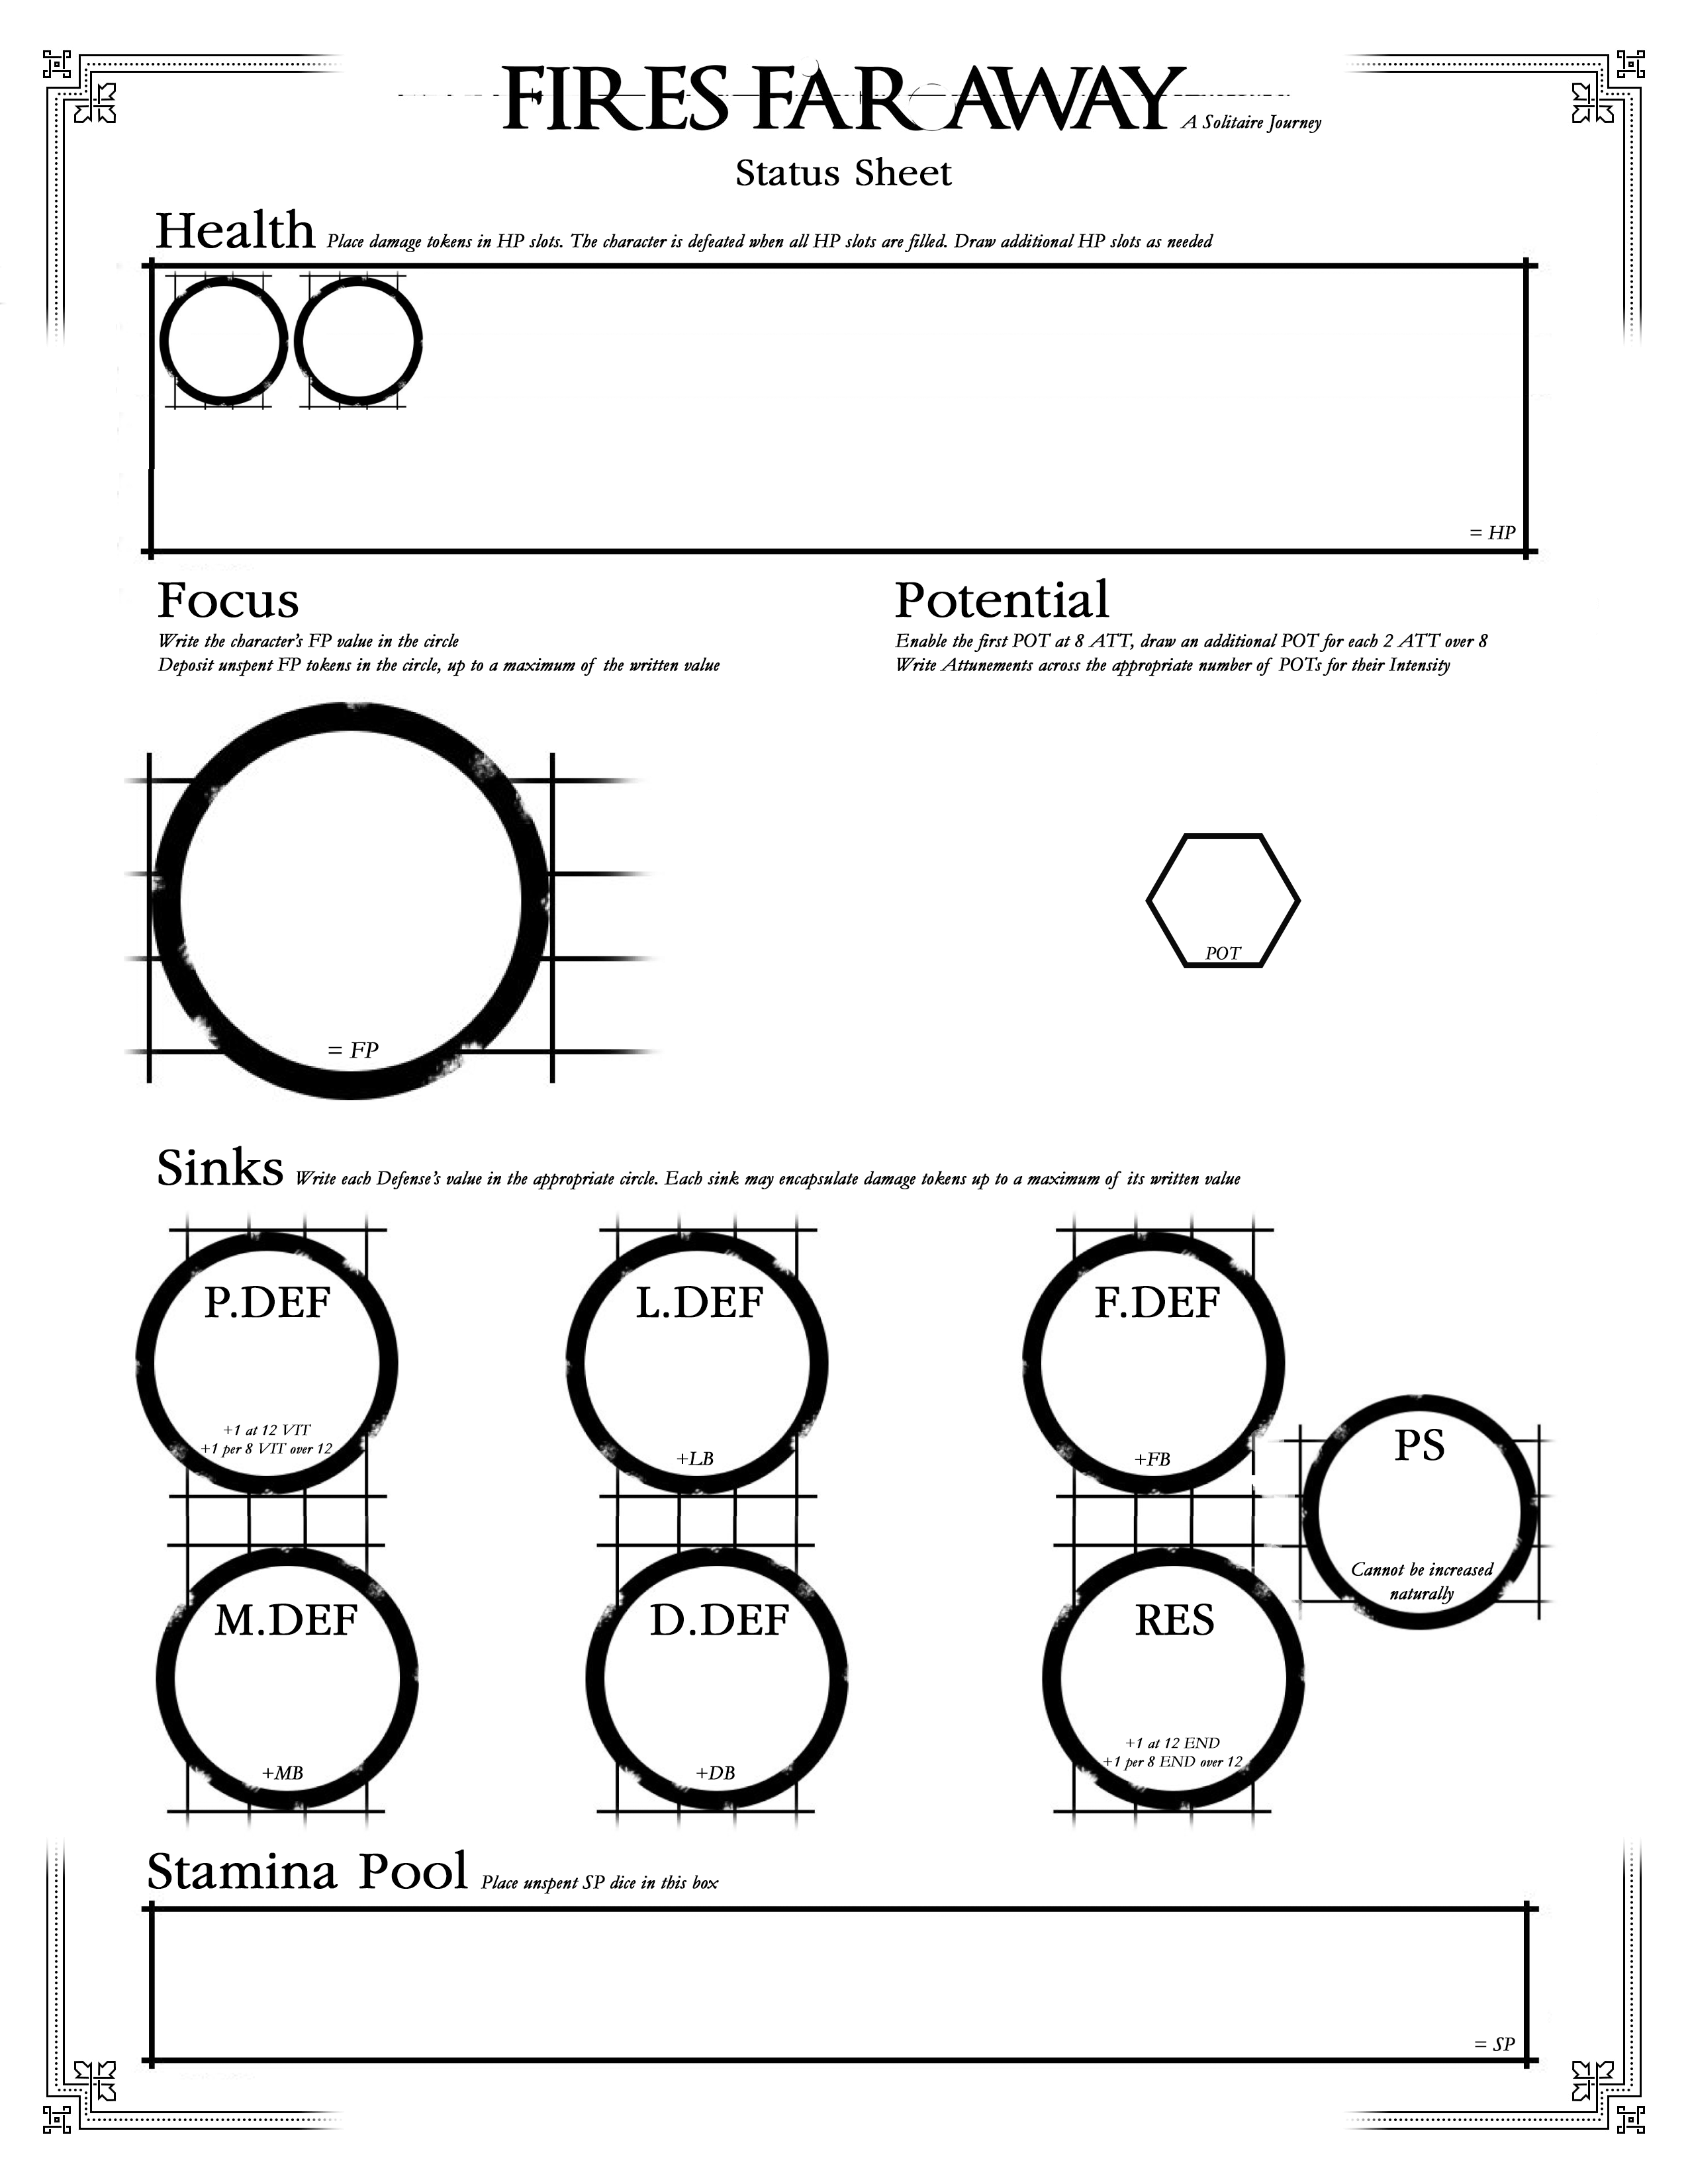
\includegraphics[width=1.22\linewidth]{misc/character_sheet_1.png}
    }
\end{center}
\newpage

\pagenumbering{gobble}
\begin{center}
\vspace*{-2.5cm}
\makebox[\linewidth]{
        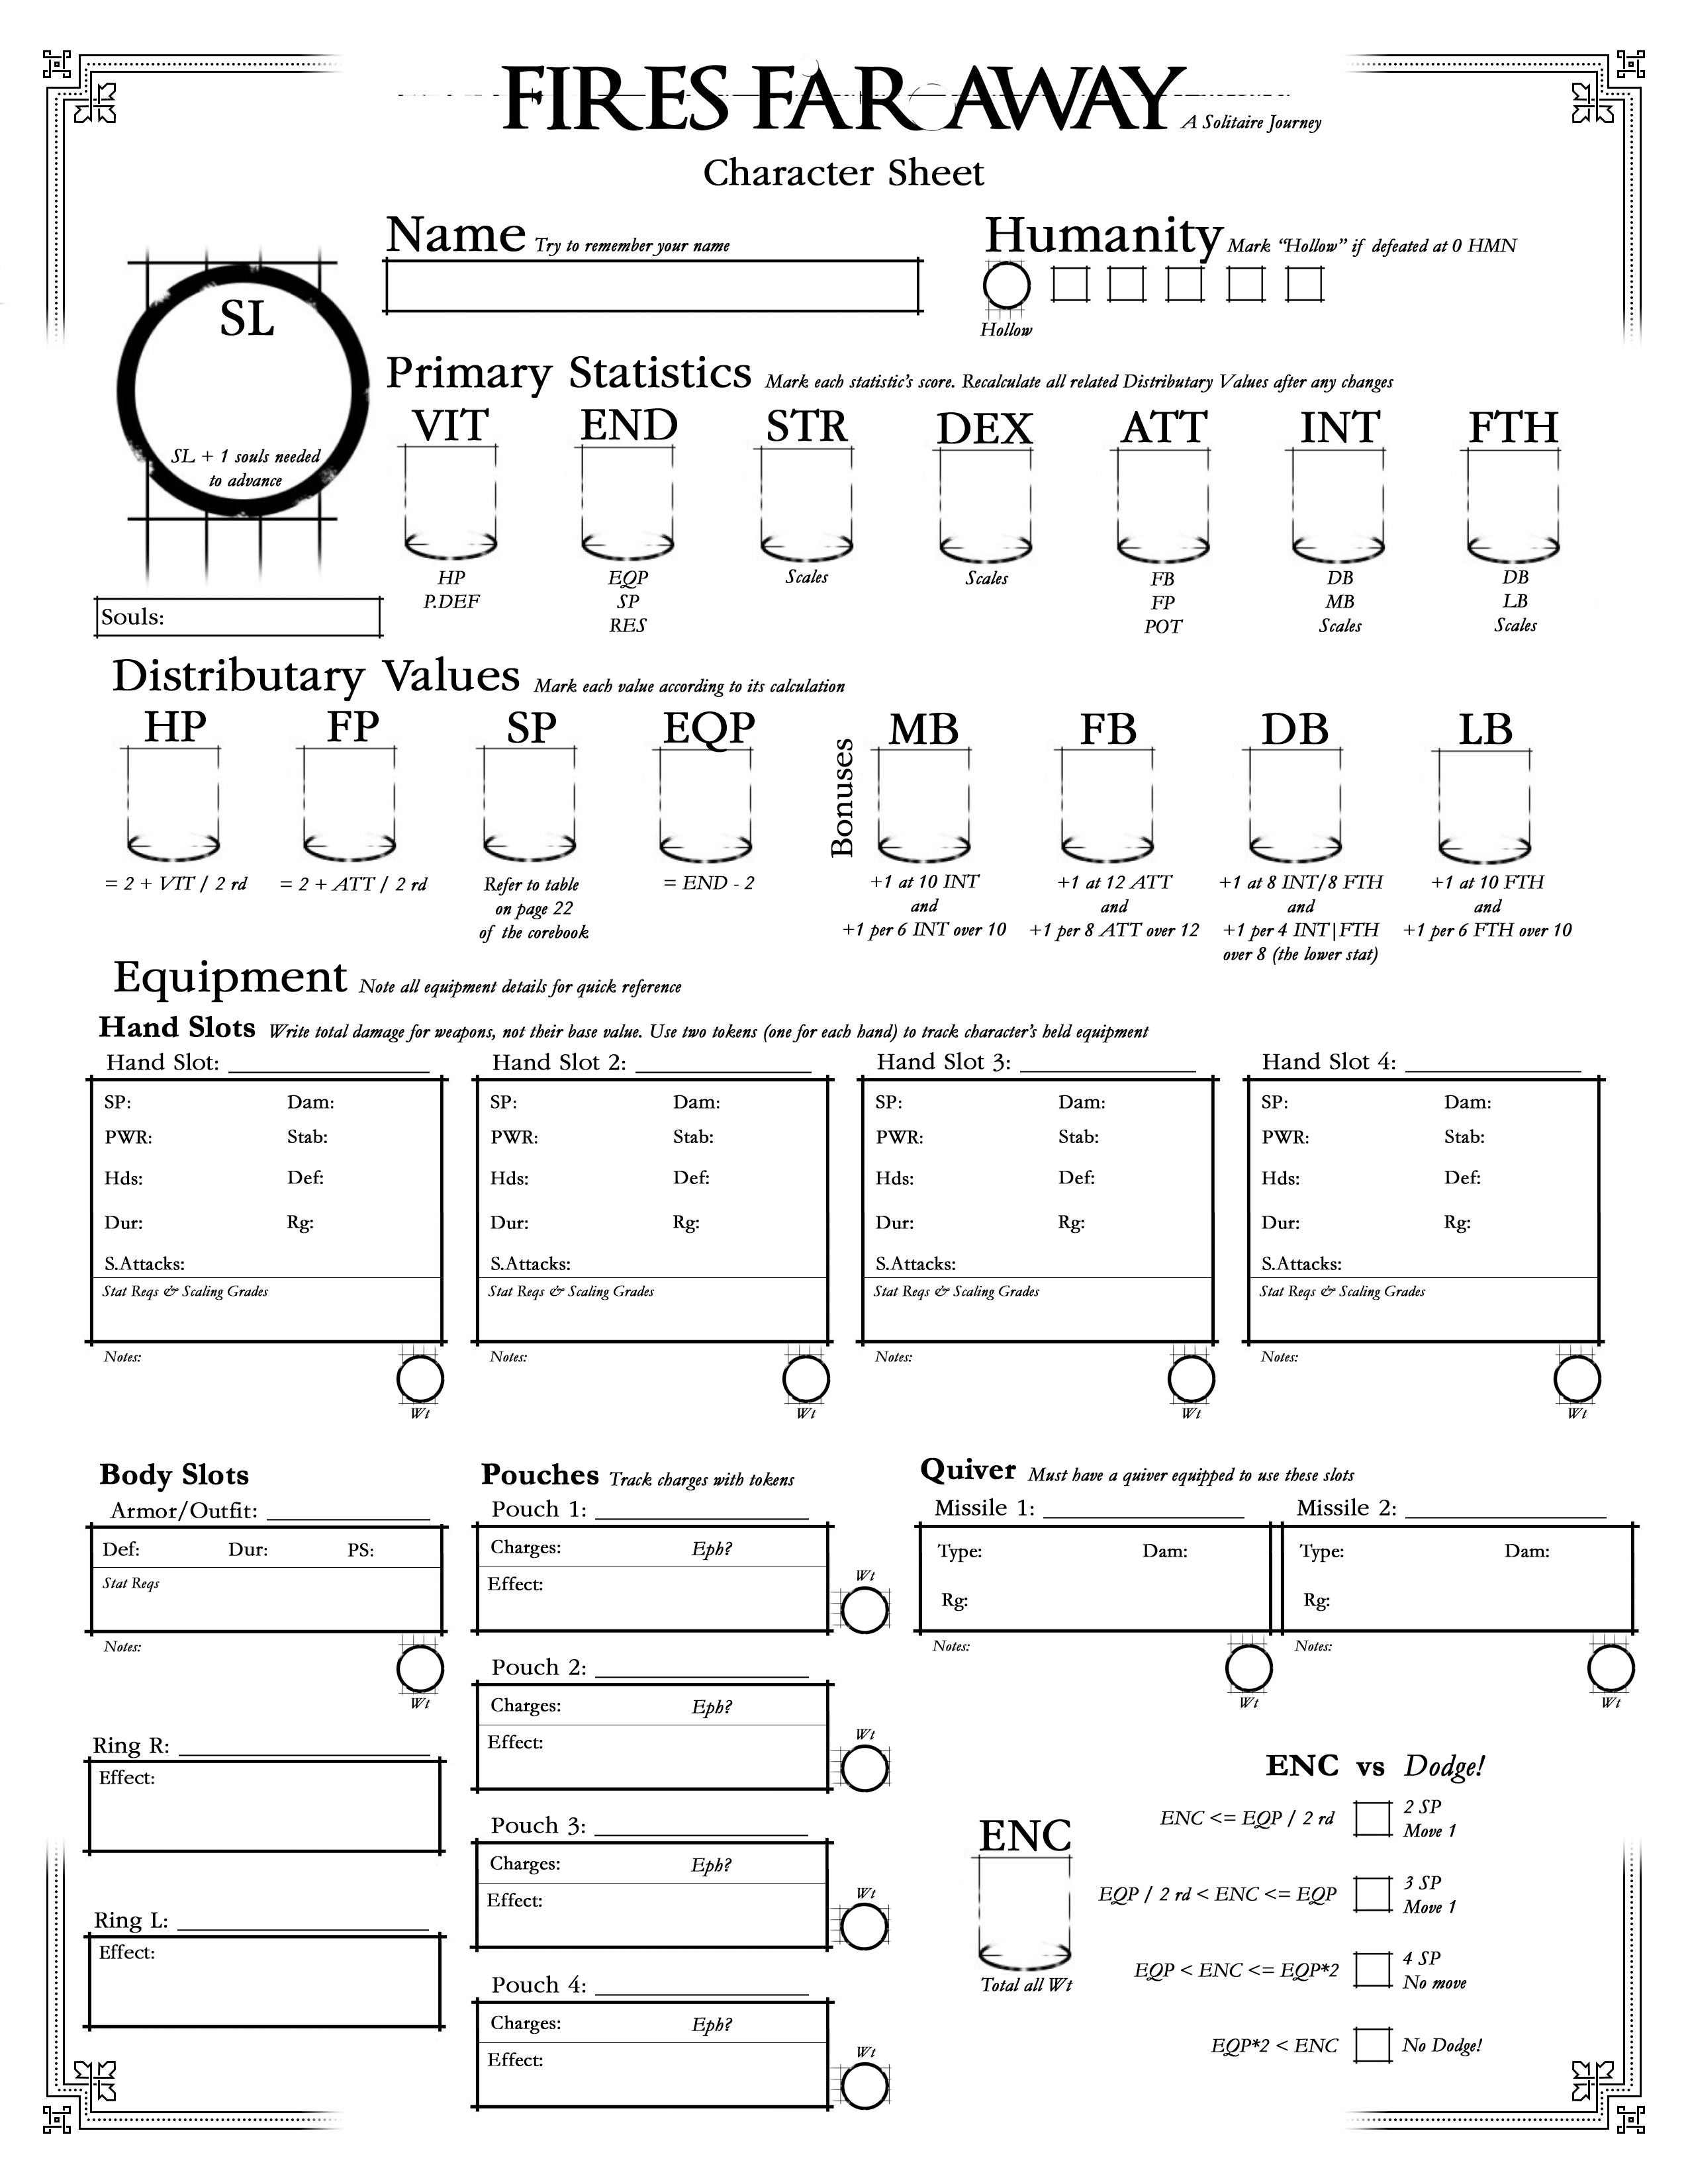
\includegraphics[width=1.22\linewidth]{misc/character_sheet_2.png}
    }
\end{center}
\newpage

\pagenumbering{gobble}
\begin{center}
\vspace*{-2.5cm}
\makebox[\linewidth]{
        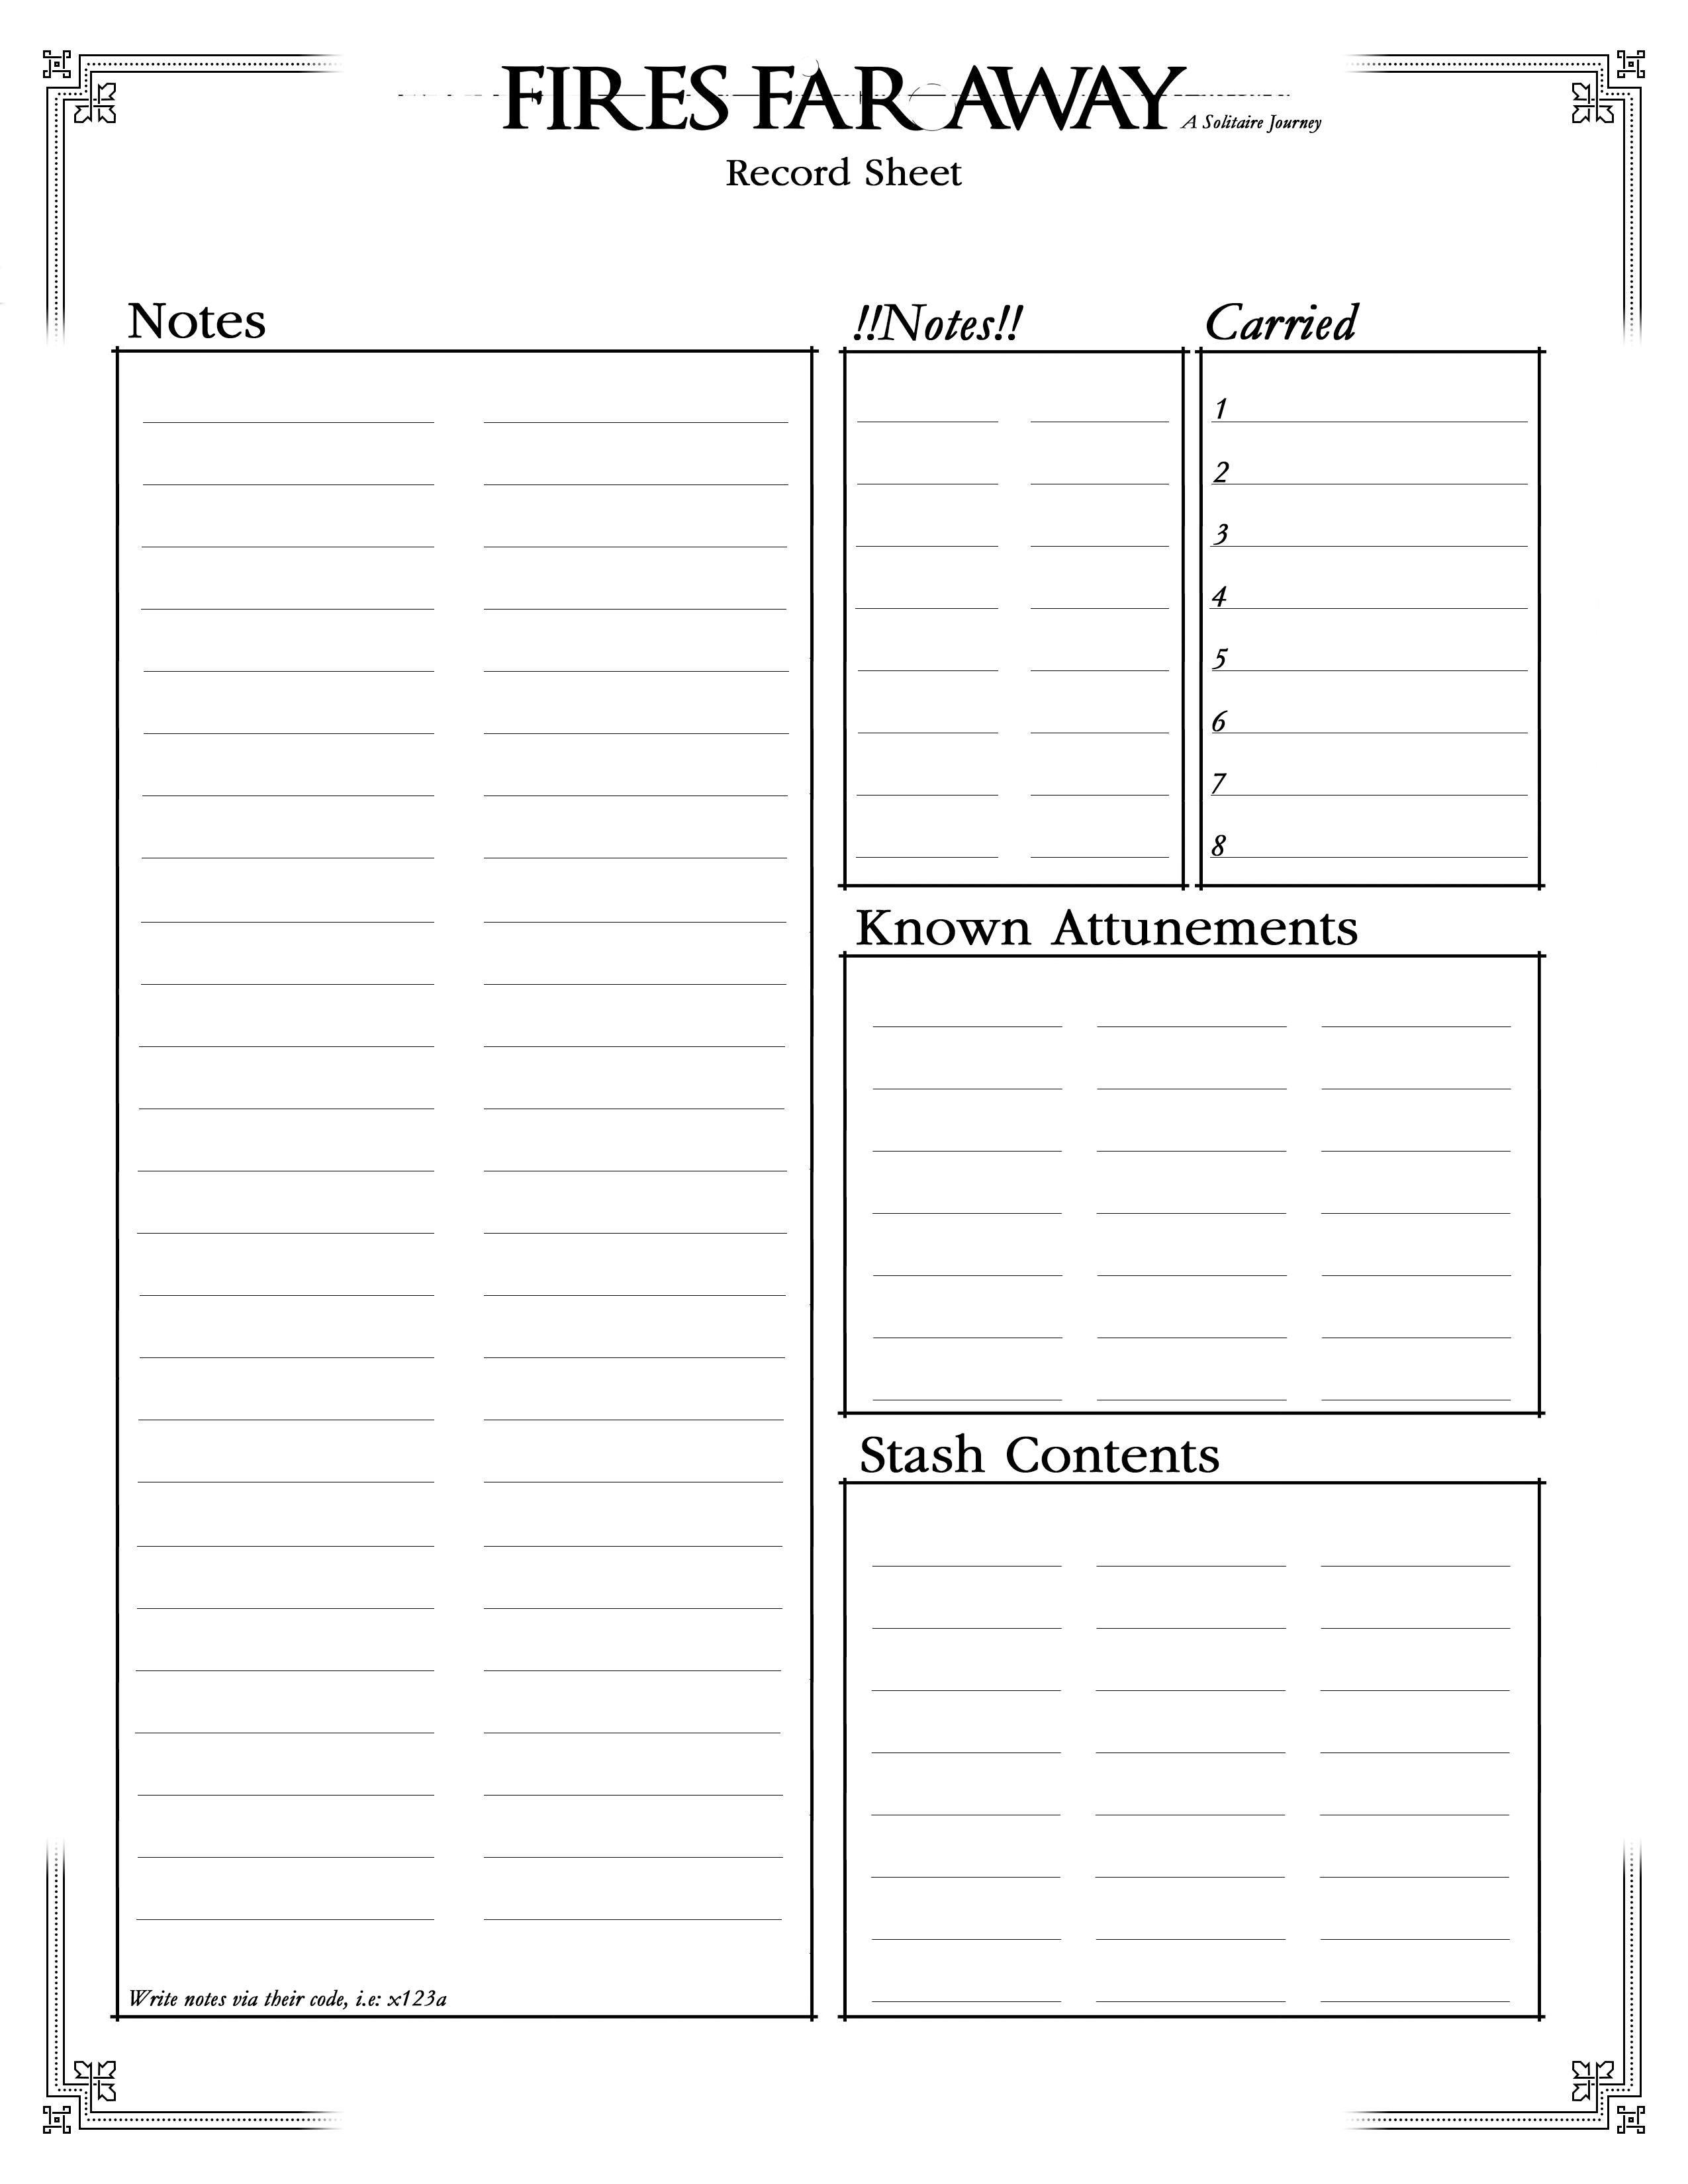
\includegraphics[width=1.22\linewidth]{misc/character_sheet_3.png}
    }
\end{center}
\newpage

\pagenumbering{gobble}
\begin{center}
\vspace*{-2.5cm}
\makebox[\linewidth]{
        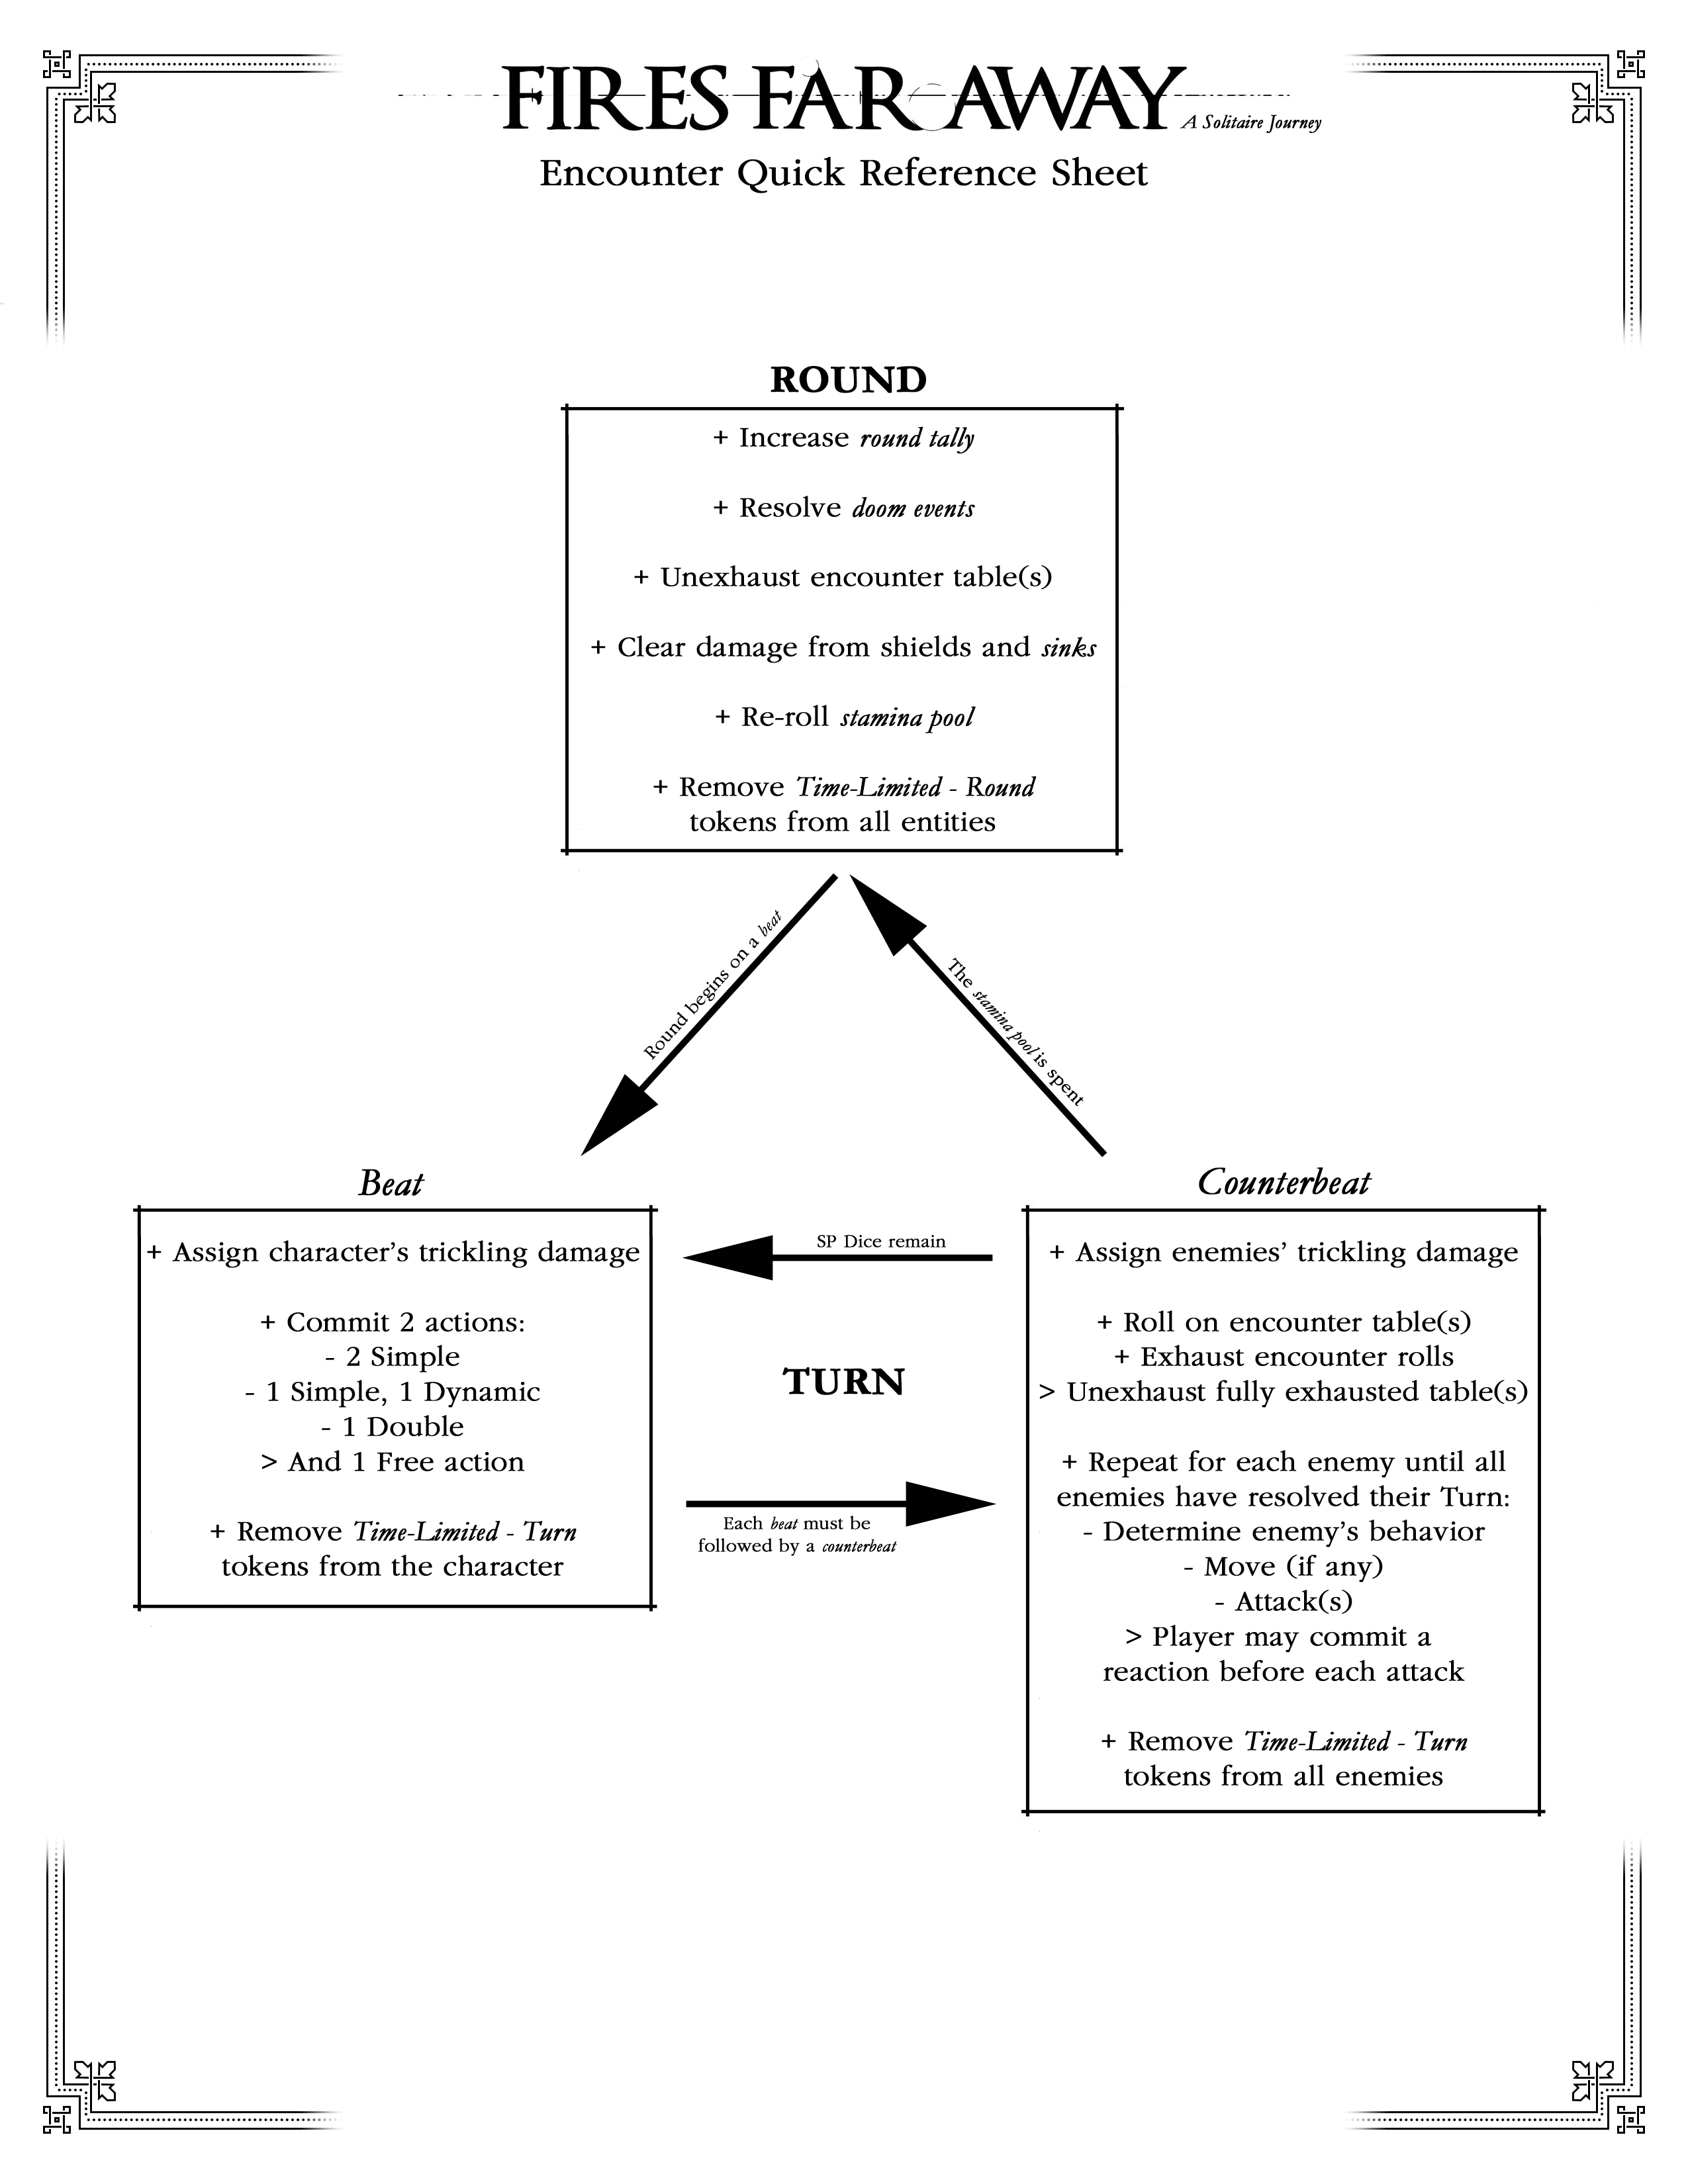
\includegraphics[width=1.22\linewidth]{misc/encounter_reference_sheet.png}
    }
\end{center}
\newpage

\ClearShipoutPicture
\pagenumbering{gobble}
\begin{center}
\vspace*{-2.1cm}
\makebox[\linewidth]{
        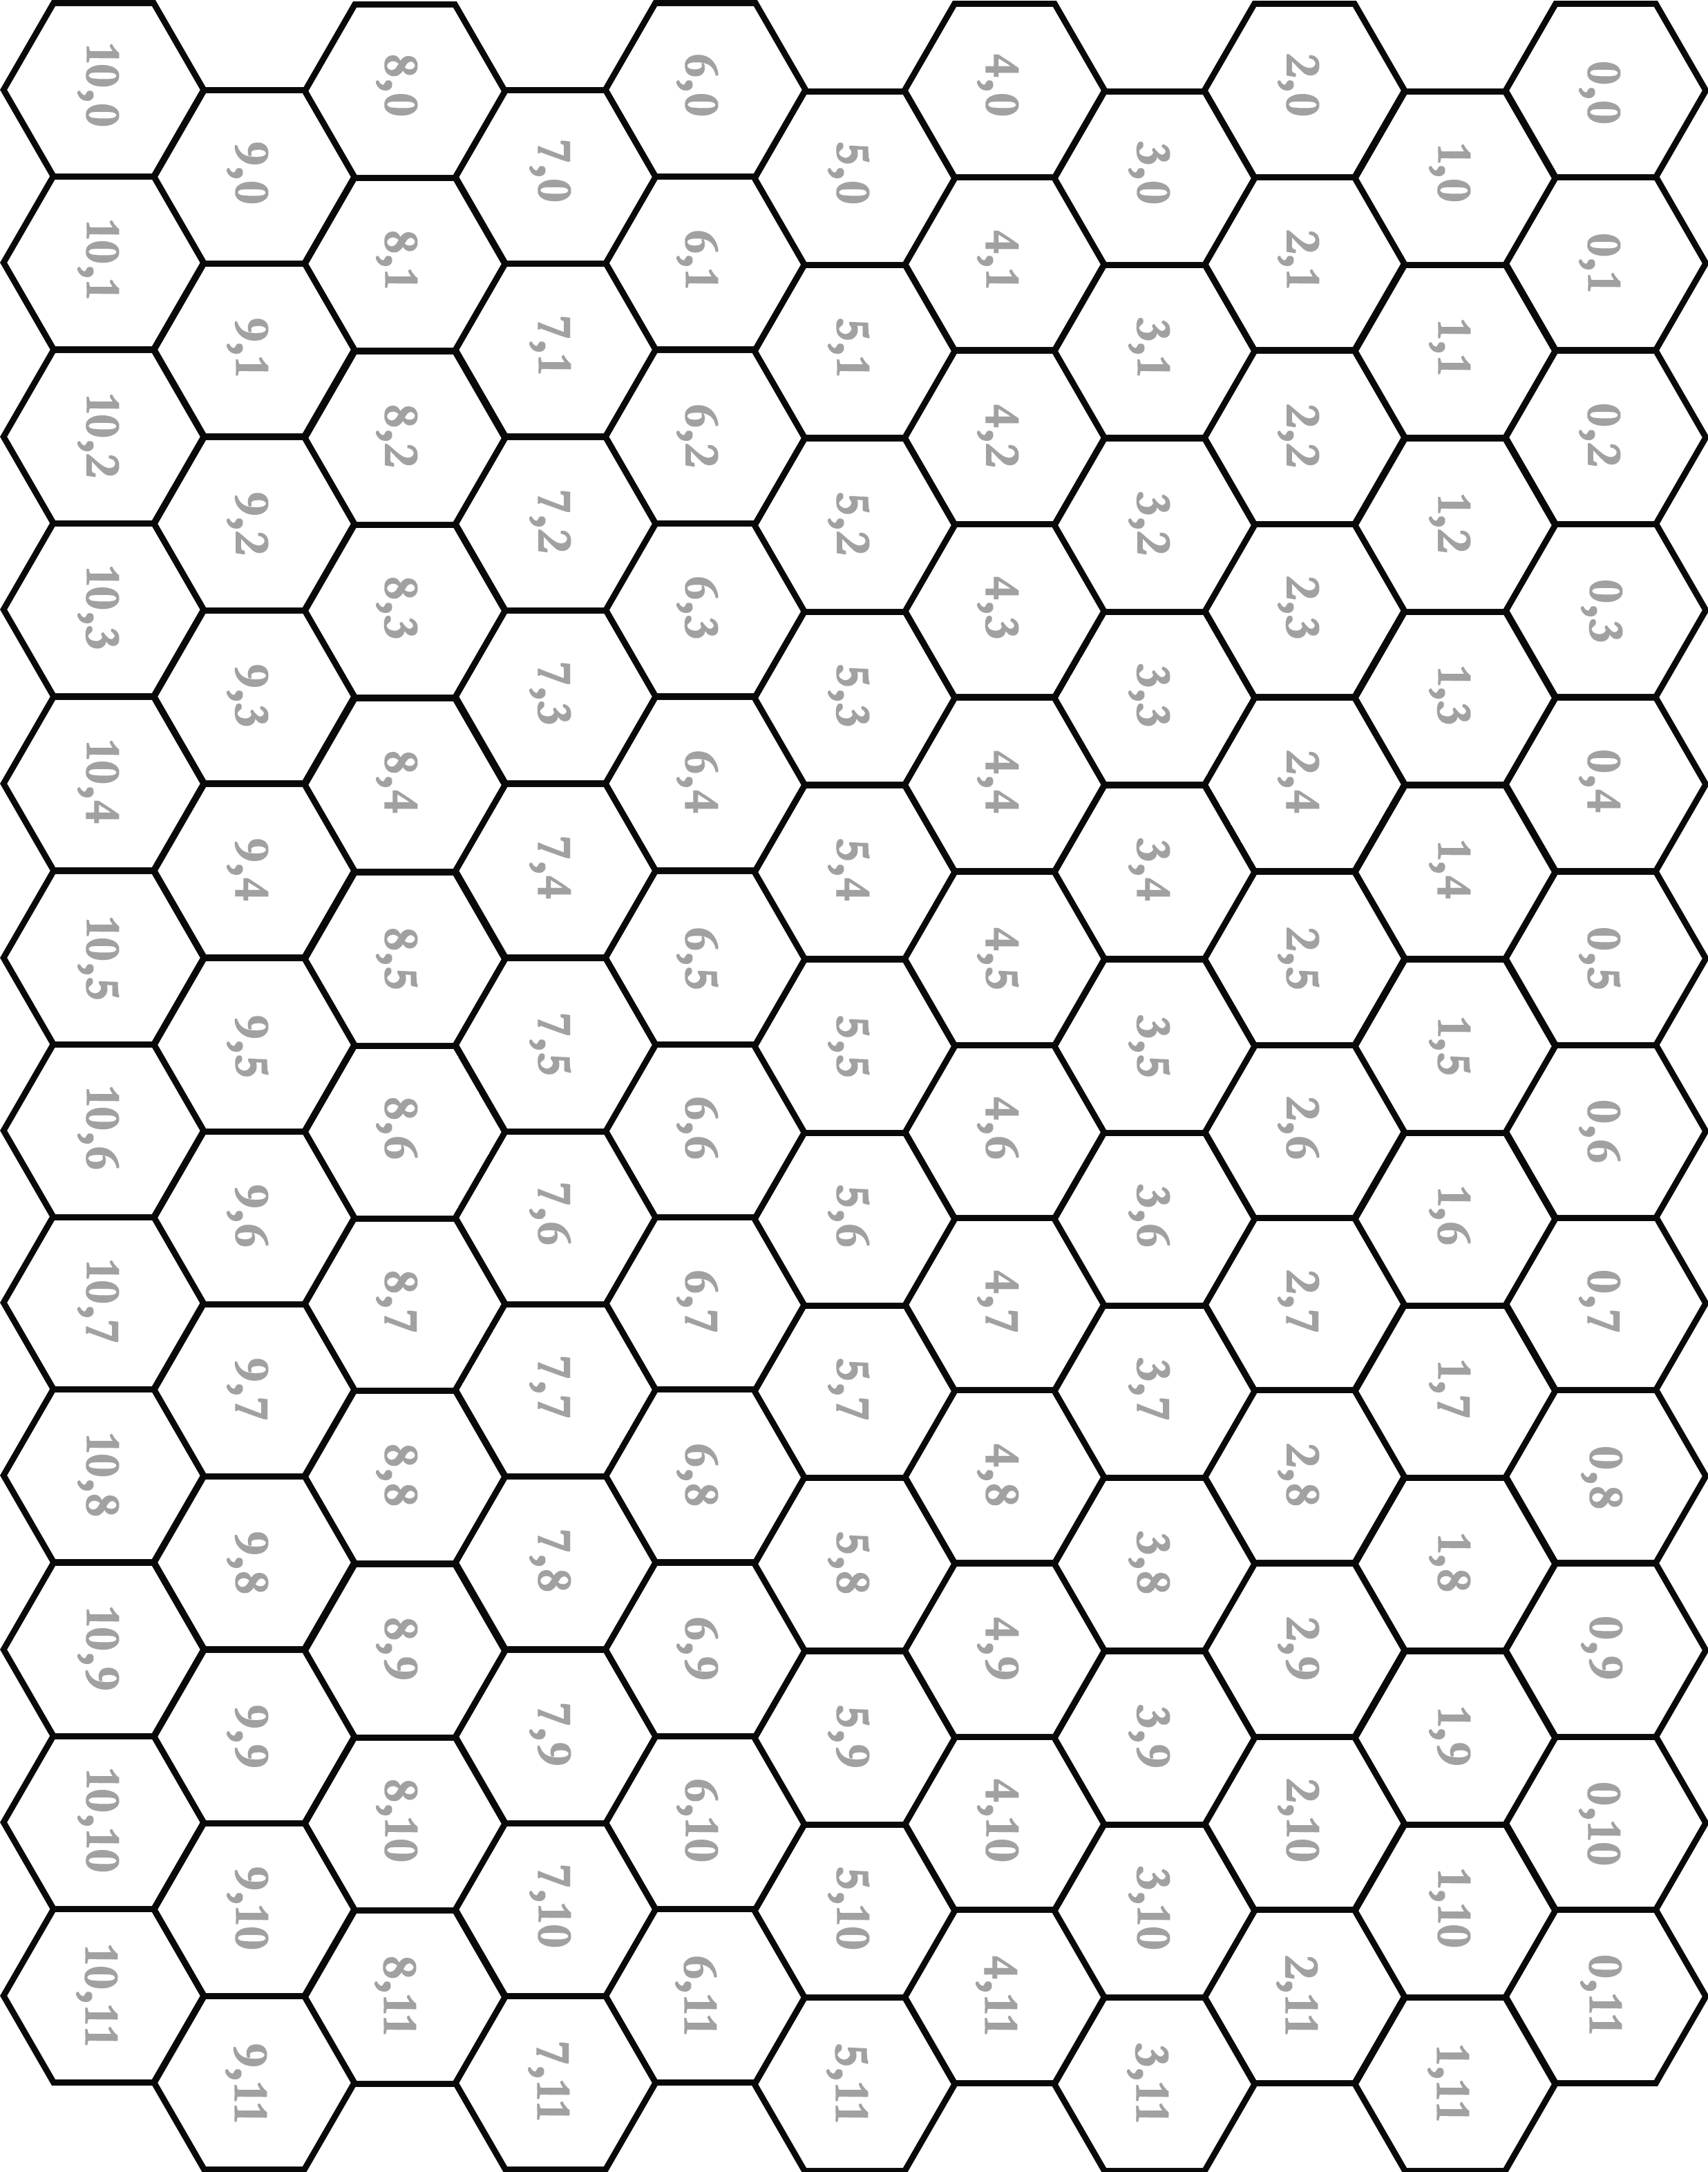
\includegraphics[width=1.214\linewidth]{misc/map.png}
    }
\end{center}
\end{document}